\documentclass[]{article}
\usepackage{lmodern}
\usepackage{amssymb,amsmath}
\usepackage{ifxetex,ifluatex}
\usepackage{fixltx2e} % provides \textsubscript
\ifnum 0\ifxetex 1\fi\ifluatex 1\fi=0 % if pdftex
  \usepackage[T1]{fontenc}
  \usepackage[utf8]{inputenc}
\else % if luatex or xelatex
  \ifxetex
    \usepackage{mathspec}
    \usepackage{xltxtra,xunicode}
  \else
    \usepackage{fontspec}
  \fi
  \defaultfontfeatures{Mapping=tex-text,Scale=MatchLowercase}
  \newcommand{\euro}{€}
\fi
% use upquote if available, for straight quotes in verbatim environments
\IfFileExists{upquote.sty}{\usepackage{upquote}}{}
% use microtype if available
\IfFileExists{microtype.sty}{%
\usepackage{microtype}
\UseMicrotypeSet[protrusion]{basicmath} % disable protrusion for tt fonts
}{}
\usepackage{color}
\usepackage{fancyvrb}
\newcommand{\VerbBar}{|}
\newcommand{\VERB}{\Verb[commandchars=\\\{\}]}
\DefineVerbatimEnvironment{Highlighting}{Verbatim}{commandchars=\\\{\}}
% Add ',fontsize=\small' for more characters per line
\usepackage{framed}
\definecolor{shadecolor}{RGB}{248,248,248}
\newenvironment{Shaded}{\begin{snugshade}}{\end{snugshade}}
\newcommand{\KeywordTok}[1]{\textcolor[rgb]{0.13,0.29,0.53}{\textbf{{#1}}}}
\newcommand{\DataTypeTok}[1]{\textcolor[rgb]{0.13,0.29,0.53}{{#1}}}
\newcommand{\DecValTok}[1]{\textcolor[rgb]{0.00,0.00,0.81}{{#1}}}
\newcommand{\BaseNTok}[1]{\textcolor[rgb]{0.00,0.00,0.81}{{#1}}}
\newcommand{\FloatTok}[1]{\textcolor[rgb]{0.00,0.00,0.81}{{#1}}}
\newcommand{\CharTok}[1]{\textcolor[rgb]{0.31,0.60,0.02}{{#1}}}
\newcommand{\StringTok}[1]{\textcolor[rgb]{0.31,0.60,0.02}{{#1}}}
\newcommand{\CommentTok}[1]{\textcolor[rgb]{0.56,0.35,0.01}{\textit{{#1}}}}
\newcommand{\OtherTok}[1]{\textcolor[rgb]{0.56,0.35,0.01}{{#1}}}
\newcommand{\AlertTok}[1]{\textcolor[rgb]{0.94,0.16,0.16}{{#1}}}
\newcommand{\FunctionTok}[1]{\textcolor[rgb]{0.00,0.00,0.00}{{#1}}}
\newcommand{\RegionMarkerTok}[1]{{#1}}
\newcommand{\ErrorTok}[1]{\textbf{{#1}}}
\newcommand{\NormalTok}[1]{{#1}}
\usepackage{longtable,booktabs}
\usepackage{graphicx}
\makeatletter
\def\maxwidth{\ifdim\Gin@nat@width>\linewidth\linewidth\else\Gin@nat@width\fi}
\def\maxheight{\ifdim\Gin@nat@height>\textheight\textheight\else\Gin@nat@height\fi}
\makeatother
% Scale images if necessary, so that they will not overflow the page
% margins by default, and it is still possible to overwrite the defaults
% using explicit options in \includegraphics[width, height, ...]{}
\setkeys{Gin}{width=\maxwidth,height=\maxheight,keepaspectratio}
\ifxetex
  \usepackage[setpagesize=false, % page size defined by xetex
              unicode=false, % unicode breaks when used with xetex
              xetex]{hyperref}
\else
  \usepackage[unicode=true]{hyperref}
\fi
\hypersetup{breaklinks=true,
            bookmarks=true,
            pdfauthor={},
            pdftitle={},
            colorlinks=true,
            citecolor=blue,
            urlcolor=blue,
            linkcolor=magenta,
            pdfborder={0 0 0}}
\urlstyle{same}  % don't use monospace font for urls
\setlength{\parindent}{0pt}
\setlength{\parskip}{6pt plus 2pt minus 1pt}
\setlength{\emergencystretch}{3em}  % prevent overfull lines
\setcounter{secnumdepth}{0}

%%% Use protect on footnotes to avoid problems with footnotes in titles
\let\rmarkdownfootnote\footnote%
\def\footnote{\protect\rmarkdownfootnote}

%%% Change title format to be more compact
\usepackage{titling}
\setlength{\droptitle}{-2em}
  \title{}
  \pretitle{\vspace{\droptitle}}
  \posttitle{}
  \author{}
  \preauthor{}\postauthor{}
  \date{}
  \predate{}\postdate{}




\begin{document}

\maketitle


{
\hypersetup{linkcolor=black}
\setcounter{tocdepth}{2}
\tableofcontents
}
\newpage

\subsection{About this book}\label{about-this-book}

This book is written as a companion book to the
\href{https://www.coursera.org/course/statinference}{Statistical
Inference} Coursera class as part of the
\href{https://www.coursera.org/specialization/jhudatascience/1?utm_medium=courseDescripTop}{Data
Science Specialization}. However, if you do not take the class, the book
mostly stands on its own. A useful component of the book is a series of
YouTube videos that comprise the Coursera class.

The book is intended to be a low cost introduction to the important
field of statistical inference. The intended audience are students who
are numerically and computationally literate, who would like to put
those skills to use in Data Science or Statistics. The book is offered
for free as a series of markdown documents on github and in more
convenient forms (epub, mobi) on LeanPub and retail outlets.

This book is licensed under a
\href{http://creativecommons.org/licenses/by-nc-sa/4.0/}{Creative
Commons Attribution-NonCommercial-ShareAlike 4.0 International License},
which requires author attribution for derivative works, non-commercial
use of derivative works and that changes are shared in the same way as
the original work.

\subsection{About the picture on the
cover}\label{about-the-picture-on-the-cover}

The picture on the cover is a public domain image taken from Wikipedia's
article on Francis Galton's quincunx. Francis Galton was an 19th century
polymath who invented many of key concepts of statistics. The quincunx
was an ingenious invention for illustrating the central limit theorem
using a pinball setup.

\newpage

\section{Introduction}\label{introduction}

\subsection{Before beginning}\label{before-beginning}

This book is designed as a companion to the
\href{https://www.coursera.org/course/statinference}{Statistical
Inference} Coursera class as part of the
\href{https://www.coursera.org/specialization/jhudatascience/1?utm_medium=courseDescripTop}{Data
Science Specialization}, a ten course program offered by three faculty,
Jeff Leek, Roger Peng and Brian Caffo, at the Johns Hopkins University
Department of Biostatistics.

The videos associated with this book
\href{https://www.youtube.com/watch?v=WkOinijQmPU\&list=PLpl-gQkQivXiBmGyzLrUjzsblmQsLtkzJ}{can
be watched in full here}, though the relevant links to specific videos
are placed at the appropriate locations throughout.

Before beginning, we assume that you have a working knowledge of the R
programming language. If not, there is a wonderful Coursera class by
Roger Peng, \href{https://www.coursera.org/course/rprog}{that can be
found here}.

The entirety of the book is on GitHub
\href{https://github.com/bcaffo/LittleInferenceBook}{here}. Please
submit pull requests if you find errata! In addition the course notes
can be found also on GitHub
\href{https://github.com/bcaffo/courses/tree/master/06_StatisticalInference}{here}.
While most code is in the book, \emph{all} of the code for every figure
and analysis in the book is in the R markdown files files (.Rmd) for the
respective lectures.

Finally, we should mention \texttt{swirl} (statistics with interactive R
programming). \texttt{swirl} is an intelligent tutoring system developed
by Nick Carchedi, with contributions by Sean Kross and Bill and Gina
Croft. It offers a way to learn R in R. Download \texttt{swirl}
\href{http://swirlstats.com}{here}. There's a swirl
\href{https://github.com/swirldev/swirl_courses\#swirl-courses}{module
for this course!}. Try it out, it's probably the most effective way to
learn.

\subsection{Statistical inference
defined}\label{statistical-inference-defined}

\href{http://youtu.be/WkOinijQmPU?list=PLpl-gQkQivXiBmGyzLrUjzsblmQsLtkzJ}{Watch
this video before beginning.}

We'll define statistical inference as the process of generating
conclusions about a population from a noisy sample. Without statistical
inference we're simply living within our data. With statistical
inference, we're trying to generate new knowledge.

Knowledge and parsimony, (using simplest reasonable models to explain
complex phenomena), go hand in hand. Probability models will serve as
our parsimonious description of the world. The use of probability models
as the connection between our data and a populations represents the most
effective way to obtain inference.

\subsubsection{Motivating example: who's going to win the
election?}\label{motivating-example-whos-going-to-win-the-election}

In every major election, pollsters would like to know, ahead of the
actual election, who's going to win. Here, the target of estimation (the
estimand) is clear, the percentage of people in a particular group
(city, state, county, country or other electoral grouping) who will vote
for each candidate.

We can not poll everyone. Even if we could, some polled may change their
vote by the time the election occurs. How do we collect a reasonable
subset of data and quantify the uncertainty in the process to produce a
good guess at who will win?

\subsubsection{Motivating example, predicting the
weather}\label{motivating-example-predicting-the-weather}

When a weatherman tells you the probability that it will rain tomorrow
is 70\%, they're trying to use historical data to predict tomorrow's
weather - and to actually attach a probability to it. That probability
talks about, refers to population.

\paragraph{Motivating example, brain
activation}\label{motivating-example-brain-activation}

An example that's very close to the research I do is trying to predict
what areas of the brain activate when a person is put in the fMRI
scanner. In that case, people are doing a task while in the scanner. For
example, they might be tapping their finger. We'd like to compare when
they are tapping their finger to when they are not tapping their finger
and try to figure out what areas of the brain are associated with the
finger tapping.

\subsection{Summary notes}\label{summary-notes}

These examples illustrate many of the difficulties of trying to use data
to create general conclusions about a population.

Paramount among our concerns are:

\begin{itemize}
\itemsep1pt\parskip0pt\parsep0pt
\item
  Is the sample representative of the population that we'd like to draw
  inferences about?
\item
  Are there known and observed, known and unobserved or unknown and
  unobserved variables that contaminate our conclusions?
\item
  Is there systematic bias created by missing data or the design or
  conduct of the study?
\item
  What randomness exists in the data and how do we use or adjust for it?
  Here randomness can either be explicit via randomization or random
  sampling, or implicit as the aggregation of many complex unknown
  processes.
\item
  Are we trying to estimate an underlying mechanistic model of phenomena
  under study?
\end{itemize}

Statistical inference requires navigating the set of assumptions and
tools and subsequently thinking about how to draw conclusions from data.

\subsection{The goals of inference}\label{the-goals-of-inference}

You should recognize the goals of inference. Here we list five examples
of inferential goals.

\begin{enumerate}
\def\labelenumi{\arabic{enumi}.}
\itemsep1pt\parskip0pt\parsep0pt
\item
  Estimate and quantify the uncertainty of an estimate of a population
  quantity (the proportion of people who will vote for a candidate).
\item
  Determine whether a population quantity is a benchmark value (``is the
  treatment effective?'').
\item
  Infer a mechanistic relationship when quantities are measured with
  noise (``What is the slope for Hooke's law?'')
\item
  Determine the impact of a policy? (``If we reduce pollution levels,
  will asthma rates decline?'')
\item
  Talk about the probability that something occurs.
\end{enumerate}

\subsection{The tools of the trade}\label{the-tools-of-the-trade}

Several tools are key to the use of statistical inference. We'll only be
able to cover a few in this class, but you should recognize them anyway.

\begin{enumerate}
\def\labelenumi{\arabic{enumi}.}
\itemsep1pt\parskip0pt\parsep0pt
\item
  \emph{Randomization}: concerned with balancing unobserved variables
  that may confound inferences of interest.
\item
  \emph{Random sampling}: concerned with obtaining data that is
  representative of the population of interest.
\item
  \emph{Sampling models}: concerned with creating a model for the
  sampling process, the most common is so called ``iid''.
\item
  \emph{Hypothesis testing}: concerned with decision making in the
  presence of uncertainty.
\item
  \emph{Confidence intervals}: concerned with quantifying uncertainty in
  estimation.
\item
  \emph{Probability models}: a formal connection between the data and a
  population of interest. Often probability models are assumed or are
  approximated.
\item
  \emph{Study design}: the process of designing an experiment to
  minimize biases and variability.
\item
  \emph{Nonparametric} bootstrapping: the process of using the data to,
  with minimal probability model assumptions, create inferences.
\item
  \emph{Permutation}, randomization and exchangeability testing: the
  process of using data permutations to perform inferences.
\end{enumerate}

\subsection{Different thinking about probability leads to different
styles of
inference}\label{different-thinking-about-probability-leads-to-different-styles-of-inference}

We won't spend too much time talking about this, but there are several
different styles of inference. Two broad categories that get discussed a
lot are:

\begin{enumerate}
\def\labelenumi{\arabic{enumi}.}
\itemsep1pt\parskip0pt\parsep0pt
\item
  \emph{Frequency probability}: is the long run proportion of times an
  event occurs in independent, identically distributed repetitions.
\item
  \emph{Frequency style inference}: uses frequency interpretations of
  probabilities to control error rates. Answers questions like ``What
  should I decide given my data controlling the long run proportion of
  mistakes I make at a tolerable level.''
\item
  \emph{Bayesian probability}: is the probability calculus of beliefs,
  given that beliefs follow certain rules.
\item
  \emph{Bayesian style inference}: the use of Bayesian probability
  representation of beliefs to perform inference. Answers questions like
  ``Given my subjective beliefs and the objective information from the
  data, what should I believe now?''
\end{enumerate}

Data scientists tend to fall within shades of gray of these and various
other schools of inference. Furthermore, there are so many shades of
gray between the styles of inferences that it is hard to pin down most
modern statisticians as either Bayesian or frequentist. In this class,
we will primarily focus on basic sampling models, basic probability
models and frequency style analyses to create standard inferences. This
is the most popular style of inference by far.

Being data scientists, we will also consider some inferential strategies
that\\rely heavily on the observed data, such as permutation testing and
bootstrapping. As probability modeling will be our starting point, we
first build up basic probability as our first task.

\subsection{Exercises}\label{exercises}

\begin{enumerate}
\def\labelenumi{\arabic{enumi}.}
\itemsep1pt\parskip0pt\parsep0pt
\item
  The goal of statistical inference is to?
\end{enumerate}

\begin{itemize}
\itemsep1pt\parskip0pt\parsep0pt
\item
  Infer facts about a population from a sample.
\item
  Infer facts about the sample from a population.
\item
  Calculate sample quantities to understand your data.
\item
  To torture Data Science students.
\end{itemize}

\begin{enumerate}
\def\labelenumi{\arabic{enumi}.}
\setcounter{enumi}{1}
\itemsep1pt\parskip0pt\parsep0pt
\item
  The goal of randomization of a treatment in a randomized trial is to?
\end{enumerate}

\begin{itemize}
\itemsep1pt\parskip0pt\parsep0pt
\item
  It doesn't really do anything.
\item
  To obtain a representative sample of subjects from the population of
  interest.
\item
  Balance unobserved covariates that may contaminate the comparison
  between the treated and control groups.
\item
  To add variation to our conclusions.
\end{itemize}

\begin{enumerate}
\def\labelenumi{\arabic{enumi}.}
\setcounter{enumi}{2}
\itemsep1pt\parskip0pt\parsep0pt
\item
  Probability is a?
\end{enumerate}

\begin{itemize}
\itemsep1pt\parskip0pt\parsep0pt
\item
  Population quantity that we can potentially estimate from data.
\item
  A data quantity that does not require the idea of a population.
\end{itemize}

\newpage

\section{Probability}\label{probability}

\href{http://youtu.be/oTERv_vrmJM?list=PLpl-gQkQivXiBmGyzLrUjzsblmQsLtkzJ}{Watch
this video before beginning.}

Probability forms the foundation for almost all treatments of
statistical inference. In our treatment, probability is a law that
assigns numbers to the long run occurrence of random phenomena after
repeated unrelated realizations.

Before we begin discussing probability, let's dispense with some deep
philosophical questions, such as ``What is randomness?'' and ``What is
the fundamental interpretation of probability?''. One could spend a
lifetime studying these questions (and some have). For our purposes,
randomness is any process occurring without apparent deterministic
patterns. Thus we will treat many things as if they were random when, in
fact they are completely deterministic. In my field, biostatistics, we
often model disease outcomes as if they were random when they are the
result of many mechanistic components whose aggregate behavior appears
random. Probability for us will be the long long run proportion of times
some occurs in repeated unrelated realizations. So, think of the
proportion of times that you get a head when flipping a coin.

For the interested student, I would recommend the books and work by Ian
Hacking to learn more about these deep philosophical issues. For us data
scientists, the above definitions will work fine.

\subsection{Where to get a more thorough treatment of
probability}\label{where-to-get-a-more-thorough-treatment-of-probability}

In this lecture, we will cover the fundamentals of probability at low
enough of a level to have a basic understanding for the rest of the
series. For a more complete treatment see the class Mathematical
Biostatistics Boot Camp 1, which can be viewed on YouTube
\href{Youtube:\%20www.youtube.com/playlist?list=PLpl-gQkQivXhk6qSyiNj51qamjAtZISJ-}{here}.
In addition, there's the actual
\href{Coursera:\%20www.coursera.org/course/biostats}{Coursera course}
that I run periodically (this is the first Coursera class that I ever
taught). Also there are a set of
\href{http://github.com/bcaffo/Caffo-Coursera}{notes on GitHub}.
Finally, there's a follow up class, uninspiringly named Mathematical
Biostatistics Boot Camp 2, that is more devoted to biostatistical topics
that has an associated
\href{http://www.youtube.com/playlist?list=PLpl-gQkQivXhwOsKPQ4fbCBYOWjvdzrSM}{YouTube
playlist}, \href{https://www.coursera.org/course/biostats2}{Coursera
Class} and
\href{https://github.com/bcaffo/MathematicsBiostatisticsBootCamp2}{GitHub
notes}.

\subsection{Kolmogorov's Three Rules}\label{kolmogorovs-three-rules}

\href{http://youtu.be/Shzt9uZ8BII?list=PLpl-gQkQivXiBmGyzLrUjzsblmQsLtkzJ}{Watch
this lecture before beginning.}

Given a random experiment (say rolling a die) a probability measure is a
population quantity that summarizes the randomness. The brilliant
discovery of the father of probability, the
\href{http://en.wikipedia.org/wiki/Andrey_Kolmogorov}{Russian
mathematician Kolmogorov}, was that to satisfy our intuition about how
probability should behave, only three rules were needed.

Consider an experiment with a random outcome. Probability takes a
possible outcome from an experiment and:

\begin{enumerate}
\def\labelenumi{\arabic{enumi}.}
\itemsep1pt\parskip0pt\parsep0pt
\item
  assigns it a number between 0 and 1
\item
  requires that the probability that something occurs is 1
\item
  required that the probability of the union of any two sets of outcomes
  that have nothing in common (mutually exclusive) is the sum of their
  respective probabilities.
\end{enumerate}

From these simple rules all of the familiar rules of probability can be
developed. This all might seem a little odd at first and so we'll build
up our intuition with some simple examples based on coin flipping and
die rolling.

I would like to reiterate the important definition that we wrote out:
\emph{mutually exclusive}. Two events are mutually exclusive if they
cannot both simultaneously occur. For example, we cannot simultaneously
get a 1 and a 2 on a die. Rule 3 says that since the event of getting a
1 and 2 on a die are mutually exclusive, the probability of getting at
least one (the union) is the sum of their probabilities. So if we know
that the probability of getting a 1 is 1/6 and the probability of
getting a 2 is 1/6, then the probability of getting a 1 or a 2 is 2/6,
the sum of the two probabilities since they are mutually exclusive.

\subsection{Consequences of The Three
Rules}\label{consequences-of-the-three-rules}

Let's cover some consequences of our three simple rules. Take, for
example, the probability that something occurs is 1 minus the
probability of the opposite occurring. Let $A$ be the event that we get
a 1 or a 2 on a rolled die. Then $A^c$ is the opposite, getting a 3, 4,
5 or 6. Since $A$ and $A^c$ cannot both simultaneously occur, they are
mutually exclusive. So the probability that either $A$ or $A^c$ is
$P(A) + P(A^c)$. Notice, that the probability that either occurs is the
probability of getting a 1, 2, 3, 4, 5 or 6, or in other words, the
probability that something occurs, which is 1 by rule number 2. So we
have that $1 = P(A) + P(A^c)$ or that $P(A) = 1 - P(A^c)$.

We won't go through this tedious exercise (since Kolmogorov already did
it for us). Instead here's a list of some of the consequences of
Kolmogorov's rules that are often useful.

\begin{enumerate}
\def\labelenumi{\arabic{enumi}.}
\itemsep1pt\parskip0pt\parsep0pt
\item
  The probability that nothing occurs is 0
\item
  The probability that something occurs is 1
\item
  The probability of something is 1 minus the probability that the
  opposite occurs
\item
  The probability of at least one of two (or more) things that can not
  simultaneously occur (mutually exclusive) is the sum of their
  respective probabilities
\item
  For any two events the probability that at least one occurs is the sum
  of their probabilities minus their intersection.
\end{enumerate}

This last rules states that $P(A \cup B) = P(A) + P(B)  - P(A \cap B)$
shows what is the issue with adding probabilities that are not mutually
exclusive. If we do this, we've added the probability that both occur in
twice! (Watch the video where I draw a Venn diagram to illustrate this).

\subsubsection{Example of Implementing Probability
Calculus}\label{example-of-implementing-probability-calculus}

The National Sleep Foundation
(\href{http://www.sleepfoundation.org/}{www.sleepfoundation.org})
reports that around 3\% of the American population has sleep apnea. They
also report that around 10\% of the North American and European
population has restless leg syndrome. Does this imply that 13\% of
people will have at least one sleep problems of these sorts? In other
words, can we simply add these two probabilities?

Answer: No, the events can simultaneously occur and so are not mutually
exclusive. To elaborate let:

\begin{eqnarray*}
     A_1 & = & \{\mbox{Person has sleep apnea}\} \\
A_2 & = & \{\mbox{Person has RLS}\}
   \end{eqnarray*}

Then

\begin{eqnarray*}
     P(A_1 \cup A_2 ) & = & P(A_1) + P(A_2) - P(A_1 \cap
A_2) \\
    & = & 0.13 - \mbox{Probability of having both}
   \end{eqnarray*}

Given the scenario, it's likely that some fraction of the population has
both. This example serves as a reminder \emph{don't add probabilities
unless the events are mutually exclusive}. We'll have a similar rule for
multiplying probabilities and independence.

\subsection{Random variables}\label{random-variables}

\href{http://youtu.be/Shzt9uZ8BII?list=PLpl-gQkQivXiBmGyzLrUjzsblmQsLtkzJ}{Watch
this video before reading this section}

Probability calculus is useful for understanding the rules that
probabilities must follow. However, we need ways to model and think
about probabilities for numeric outcomes of experiments (broadly
defined). Densities and mass functions for random variables are the best
starting point for this. You've already heard of a density since you've
heard of the famous ``bell curve'', or Gaussian density. In this section
you'll learn exactly what the bell curve is and how to work with it.

Remember, everything we're talking about up to at this point is a
population quantity, not a statement about what occurs in our data.
Think about the fact that 50\% probability for head is a statement about
the coin and how we're flipping it, not a statement about the percentage
of heads we obtained in a particular set of flips. This is an important
distinction that we will emphasize over and over in this course.
Statistical inference is about describing populations using data.
Probability density functions are a way to mathematically characterize
the population. In this course, we'll assume that our sample is a random
draw from the population.

So our definition is that a \textbf{random variable} is a numerical
outcome of an experiment. The random variables that we study will come
in two varieties, \textbf{discrete} or \textbf{continuous}. Discrete
random variable are random variables that take on only a countable
number of possibilities. Mass functions will assign probabilities that
they take specific values. Continuous random variable can conceptually
take any value on the real line or some subset of the real line and we
talk about the probability that they line within some range. Densities
will characterize these probabilities.

Let's consider some examples of measurements that could be considered
random variables. First, familiar gambling experiments like the tossing
of a coin and the rolling of a die produce random variables. For the
coin, we typically code a tail as a 0 and a head as a 1. (For the die,
the number facing up would be the random variable.) We will use these
examples a lot to help us build intuition. However, they aren't
interesting in the sense of seeming very contrived. Nonetheless, the
coin example is particularly useful since many of the experiments we
consider will be modeled as if tossing a biased coin. Modeling any
binary characteristic from a random sample of a population can be
thought of as a coin toss, with the random sampling performing the roll
of the toss and the population percentage of individuals with the
characteristic is the probability of a head. Consider, for example,
logging whether or not subjects were hypertensive in a random sample.
Each subject's outcome can be modeled as a coin toss. In a similar sense
the die roll serves as our model for phenomena with more than one level,
such as hair color or rating scales.

Consider also the random variable of the number of web hits for a site
each day. This variable is a count, but is largely unbounded (or at
least we couldn't put a specific reasonable upper limit). Random
variables like this are often modeled with the so called Poisson
distribution.

Finally, consider some continuous random variables. Think of things like
lengths or weights. It is mathematically convenient to model these as if
they were continuous (even if measurements were truncated liberally). In
fact, even discrete random variables with lots of levels are often
treated as continuous for convenience.

For all of these kinds of random variables, we need convenient
mathematical functions to model the probabilities of collections of
realizations. These functions, called mass functions and densities, take
possible values of the random variables, and assign the associated
probabilities. These entities describe the population of interest. So,
consider the most famous density, the normal distribution. Saying that
body mass indices follow a normal distribution is a statement about the
population of interest. The goal is to use our data to figure out things
about that normal distribution, where it's centered, how spread out it
is and even whether our assumption of normality is warranted!

\subsection{Probability mass
functions}\label{probability-mass-functions}

A probability mass function evaluated at a value corresponds to the
probability that a random variable takes that value. To be a valid pmf a
function, $p$, must satisfy:

\begin{enumerate}
\def\labelenumi{\arabic{enumi}.}
\itemsep1pt\parskip0pt\parsep0pt
\item
  It must always be larger than or equal to 0.
\item
  The sum of the possible values that the random variable can take has
  to add up to one.
\end{enumerate}

\subsubsection{Example}\label{example}

Let $X$ be the result of a coin flip where $X=0$ represents tails and
$X = 1$ represents heads. $p(x) = (1/2)^{x} (1/2)^{1-x}$ for $x = 0,1$.
Suppose that we do not know whether or not the coin is fair; Let
$\theta$ be the probability of a head expressed as a proportion (between
0 and 1). $p(x) = \theta^{x} (1 - \theta)^{1-x}$ for $x = 0,1$

\subsection{Probability density
functions}\label{probability-density-functions}

\href{http://youtu.be/mPe0Us4VYDM?list=PLpl-gQkQivXiBmGyzLrUjzsblmQsLtkzJ}{Watch
this video before beginning.}

A probability density function (pdf), is a function associated with a
continuous random variable. Because of the peculiarities of treating
measurements as having been recorded to infinite decimal expansions, we
need a different set of rules. This leads us to the central dogma of
probability density functions:

\emph{Areas under PDFs correspond to probabilities for that random
variable}

Therefore, when one says that intelligence quotients (IQ) in population
follows a bell curve, they are saying that the probability of a randomly
selected from this population having an IQ between two values is given
by the area under the bell curve.

Not every function can be a valid probability density function. For
example, if the function dips below zero, then we could have negative
probabilities. If the function contains too much area underneath it, we
could have probabilities larger than one. The following two rules tell
us when a function is a valid probability density function.

Specifically, to be a valid pdf, a function must satisfy

\begin{enumerate}
\def\labelenumi{\arabic{enumi}.}
\itemsep1pt\parskip0pt\parsep0pt
\item
  It must be larger than or equal to zero everywhere.
\item
  The total area under it must be one.
\end{enumerate}

\subsubsection{Example}\label{example-1}

Suppose that the proportion of help calls that get addressed in a random
day by a help line is given by $f(x) = 2 x$ for $0< x < 1$. The R code
for plotting this density is

\vspace{1pc}

\verb;Code for plotting the density:;

\begin{Shaded}
\begin{Highlighting}[]
\NormalTok{x <-}\StringTok{ }\KeywordTok{c}\NormalTok{(-}\FloatTok{0.5}\NormalTok{, }\DecValTok{0}\NormalTok{, }\DecValTok{1}\NormalTok{, }\DecValTok{1}\NormalTok{, }\FloatTok{1.5}\NormalTok{)}
\NormalTok{y <-}\StringTok{ }\KeywordTok{c}\NormalTok{(}\DecValTok{0}\NormalTok{, }\DecValTok{0}\NormalTok{, }\DecValTok{2}\NormalTok{, }\DecValTok{0}\NormalTok{, }\DecValTok{0}\NormalTok{)}
\NormalTok{p <-}\StringTok{ }\KeywordTok{plot}\NormalTok{(x, y, }\DataTypeTok{lwd =} \DecValTok{3}\NormalTok{,}\DataTypeTok{frame =} \OtherTok{FALSE}\NormalTok{, }\DataTypeTok{type =} \StringTok{"l"}\NormalTok{)}
\end{Highlighting}
\end{Shaded}

The result of the code is given below.

\begin{figure}[htbp]
\centering
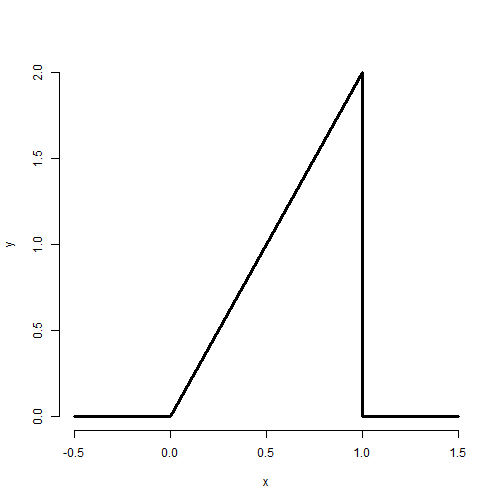
\includegraphics{LeanPub/images/triangleDensity-1.png}
\caption{Help call density}
\end{figure}

Is this a mathematically valid density? To answer this we need to make
sure it satisfies our two conditions. First it's clearly nonnegative
(it's at or above the horizontal axis everywhere). The area is similarly
easy. Being a right triangle in the only section of the density that is
above zero, we can calculate it as 1/2 the area of the base times the
height. This is $\frac{1}{2} \times 1 \times 2 = 1$

Now consider answering the following question. What is the probability
that 75\% or fewer of calls get addressed? Remember, for continuous
random variables, probabilities are represented by areas underneath the
density function. So, we want the area from 0.75 and below, as
illustrated by the figure below.

\begin{figure}[htbp]
\centering
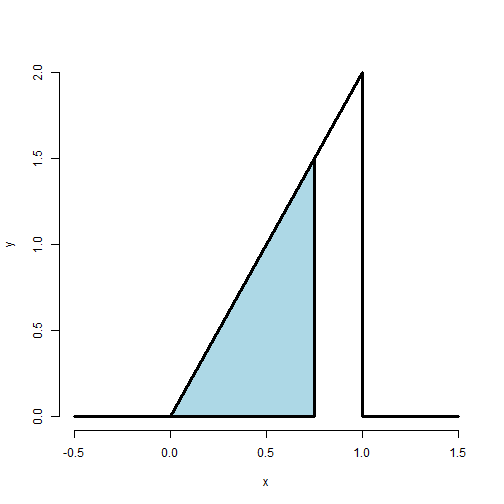
\includegraphics{LeanPub/images/triangleDensityArea-1.png}
\caption{Help call density}
\end{figure}

This again is a right triangle, with length of the base as 0.75 and
height 1.5. The R code below shows the calculation.

\begin{Shaded}
\begin{Highlighting}[]
\FloatTok{1.5} \NormalTok{*}\StringTok{ }\FloatTok{0.75}\NormalTok{/}\DecValTok{2}
\end{Highlighting}
\end{Shaded}

\begin{verbatim}
## [1] 0.5625
\end{verbatim}

Thus, the probability of 75\% or fewer calls getting addressed in a
random day for this help line is 56\%. We'll do this a lot throughout
this class and work with more useful densities. It should be noted that
this specific density is a special case of the so called \emph{beta}
density. Below I show how to use R's built in evaluation function for
the beta density to get the probability.

\begin{Shaded}
\begin{Highlighting}[]
\KeywordTok{pbeta}\NormalTok{(}\FloatTok{0.75}\NormalTok{, }\DecValTok{2}\NormalTok{, }\DecValTok{1}\NormalTok{)}
\end{Highlighting}
\end{Shaded}

\begin{verbatim}
## [1] 0.5625
\end{verbatim}

Notice the syntax \texttt{pbeta}. In R, a prefix of \texttt{p} returns
probabilities, \texttt{d} returns the density, \texttt{q} returns the
quantile and \texttt{r} returns generated random variables. (You'll
learn what each of these does in subsequent sections.)

\subsection{CDF and survival function}\label{cdf-and-survival-function}

Certain areas of PDFs and PMFs are so useful, we give them names. The
\textbf{cumulative distribution function} (CDF) of a random variable,
$X$, returns the probability that the random variable is less than or
equal to the value $x$. Notice the (slightly annoying) convention that
we use an upper case $X$ to denote a random, unrealized, version of the
random variable and a lowercase $x$ to denote a specific number that we
plug into. (This notation, as odd as it may seem, dates back to Fisher
and isn't going anywhere, so you might as well get used to it. Uppercase
for unrealized random variables and lowercase as placeholders for
numbers to plug into.) So we could write the following to describe the
distribution function $F$:

\[
F(x) = P(X \leq x)
\]

This definition applies regardless of\\whether the random variable is
discrete or continuous. The \textbf{survival function} of a random
variable $X$ is defined as the probability that the random variable is
greater than the value $x$.

\[
S(x) = P(X > x)
\]

Notice that $S(x) = 1 - F(x)$, since the survival function evaluated at
a particular value of $x$ is calculating the probability of the opposite
event (greater than as opposed to less than or equal to). The survival
function is often preferred in biostatistical applications while the
distribution function is more generally used (though both convey the
same information.)

\subsubsection{Example}\label{example-2}

What are the survival function and CDF from the density considered
before?

\[
F(x) = P(X \leq x) = \frac{1}{2} Base \times Height = \frac{1}{2} (x) \times (2 x) = x^2,
\]

for $1 \geq x \geq 0$. Notice that calculating the survival function is
now trivial given that we've already calculated the distribution
function.

\[
 S(x) = 1 = F(x) = 1 - x^2
\]

Again, R has a function that calculates the distribution function for us
in this case, \texttt{pbeta}. Let's try calculating $F(.4)$, $F(.5)$ and
$F(.6)$

\begin{Shaded}
\begin{Highlighting}[]
\KeywordTok{pbeta}\NormalTok{(}\KeywordTok{c}\NormalTok{(}\FloatTok{0.4}\NormalTok{, }\FloatTok{0.5}\NormalTok{, }\FloatTok{0.6}\NormalTok{), }\DecValTok{2}\NormalTok{, }\DecValTok{1}\NormalTok{)}
\end{Highlighting}
\end{Shaded}

\begin{verbatim}
## [1] 0.16 0.25 0.36
\end{verbatim}

Notice, of course, these are simply the numbers squared. By default the
prefix \texttt{p} in front of a density in R gives the distribution
function (\texttt{pbeta}, \texttt{pnorm}, \texttt{pgamma}). If you want
the survival function values, you could always subtract by one, or give
the argument \texttt{lower.tail = FALSE} as an argument to the function,
which asks R to calculate the upper area instead of the lower.

\subsection{Quantiles}\label{quantiles}

You've heard of sample quantiles. If you were the 95th percentile on an
exam, you know that 95\% of people scored worse than you and 5\% scored
better. These are sample quantities. But you might have wondered, what
are my sample quantiles estimating? In fact, they are estimating the
population quantiles. Here we define these population analogs.

The $\alpha^{th}$ \textbf{quantile} of a distribution with distribution
function $F$ is the point $x_\alpha$ so that

\[
F(x_\alpha) = \alpha
\]

So the 0.95 quantile of a distribution is the point so that 95\% of the
mass of the density lies below it. Or, in other words, the point so that
the probability of getting a randomly sampled point below it is 0.95.
This is analogous to the sample quantiles where the 0.95 sample quantile
is the value so that 95\% of the data lies below it.

A \textbf{percentile} is simply a quantile with $\alpha$ expressed as a
percent rather than a proportion. The (population) \textbf{median} is
the $50^{th}$ percentile. Remember that percentiles are not
probabilities! Remember that quantiles have units. So the population
median height is the height (in inches say) so that the probability that
a randomly selected person from the population is shorter is 50\%. The
sample, or empirical, median would be the height so in a sample so that
50\% of the people in the sample were shorter.

\subsubsection{Example}\label{example-3}

What is the median of the distribution that we were working with before?
We want to solve $0.5 = F(x) = x^2$, resulting in the solution

\begin{Shaded}
\begin{Highlighting}[]
\KeywordTok{sqrt}\NormalTok{(}\FloatTok{0.5}\NormalTok{)}
\end{Highlighting}
\end{Shaded}

\begin{verbatim}
## [1] 0.7071068
\end{verbatim}

Therefore, 0.7071 of calls being answered on a random day is the median.
Or, the probability that 70\% or fewer calls get answered is 50\%.

R can approximate quantiles for you for common distributions with the
prefix \texttt{q} in front of the distribution name

\begin{Shaded}
\begin{Highlighting}[]
\KeywordTok{qbeta}\NormalTok{(}\FloatTok{0.5}\NormalTok{, }\DecValTok{2}\NormalTok{, }\DecValTok{1}\NormalTok{)}
\end{Highlighting}
\end{Shaded}

\begin{verbatim}
## [1] 0.7071068
\end{verbatim}

\subsection{Exercises}\label{exercises-1}

\begin{enumerate}
\def\labelenumi{\arabic{enumi}.}
\itemsep1pt\parskip0pt\parsep0pt
\item
  Can you add the probabilities of any to events to get the probability
  of at least one occurring?
\item
  I define a PMF, $p$ so that for $x = 0$ and $x=1$ we have
  $p(0) = -0.1$ and $p(1)  = 1.1$. Is this a valid PMF?
\item
  What is the probability that 75\% or fewer calls get answered in a
  randomly sampled day from the population distribution from this
  chapter?
\item
  The 97.5th percentile of a distribution is?
\item
  Consider influenza epidemics for two parent heterosexual families.
  Suppose that the probability is 15\% that at least one of the parents
  has contracted the disease. The probability that the father has
  contracted influenza is 10\% while that the mother contracted the
  disease is 9\%. What is the probability that both contracted influenza
  expressed as a whole number percentage?
  \href{http://youtu.be/CvnmoCuIN08?list=PLpl-gQkQivXhHOcVeU3bSJg78zaDYbP9L}{Watch
  a video solution to this problem.} and
  \href{http://bcaffo.github.io/courses/06_StatisticalInference/homework/hw1.html\#3}{see
  a written out solution.}
\item
  A random variable, $X$, is uniform, a box from 0 to 1 of height 1. (So
  that it's density is $f(x) = 1$ for $0\leq x \leq 1$.) What is it's
  median expressed to two decimal places?
  \href{http://youtu.be/UXcarD-1xAM?list=PLpl-gQkQivXhHOcVeU3bSJg78zaDYbP9L}{Watch
  a video solution to this problem here} and
  \href{http://bcaffo.github.io/courses/06_StatisticalInference/homework/hw1.html\#4}{see
  written solutions here}.
\item
  If a continuous density that never touches the horizontal axis is
  symmetric about zero, can we say that its associated median is zero?
  \href{http://youtu.be/sn48CGH_TXI?list=PLpl-gQkQivXhHOcVeU3bSJg78zaDYbP9L}{Watch
  a worked out solution to this problem here} and
  \href{http://bcaffo.github.io/courses/06_StatisticalInference/homework/hw1.html\#9}{see
  the question and a typed up answer here}
\end{enumerate}

\newpage

\section{Conditional probability}\label{conditional-probability}

\subsection{Conditional probability,
motivation}\label{conditional-probability-motivation}

\href{http://youtu.be/u6AH6qsSVA4?list=PLpl-gQkQivXiBmGyzLrUjzsblmQsLtkzJ}{Watch
this video before beginning.}

Conditioning is a central subject in statistics. If we are given
information about a random variable, it changes the probabilities
associated with it. For example, the probability of getting a one when
rolling a (standard) die is usually assumed to be one sixth. If you were
given the extra information that the die roll was an odd number (hence
1, 3 or 5) then \emph{conditional on this new information}, the
probability of a one is now one third.

This is the idea of conditioning, taking away the randomness that we
know to have occurred. Consider another example, such as the result of a
diagnostic imaging test for lung cancer. What's the probability that a
person has cancer given a positive test? How does that probability
change under the knowledge that a patient has been a lifetime heavy
smoker and both of their parents had lung cancer? \emph{Conditional} on
this new information, the probability has increased dramatically.

\subsection{Conditional probability,
definition}\label{conditional-probability-definition}

We can formalize the definition of conditional probability so that the
mathematics matches our intuition.

Let $B$ be an event so that $P(B) > 0$. Then the conditional probability
of an event $A$ given that $B$ has occurred is:

\[
P(A ~|~ B) = \frac{P(A \cap B)}{P(B)}.
\]

If $A$ and $B$ are unrelated in any way, or in other words
\emph{independent}, (discussed more later in the lecture), then

\[
P(A ~|~ B) = \frac{P(A) P(B)}{P(B)} = P(A)
\]

That is, if the occurrence of $B$ offers no information about the
occurrence of $A$ - the probability conditional on the information is
the same as the probability without the information, we say that the two
events are independent.

\subsubsection{Example}\label{example-4}

Consider our die roll example again. Here we have that $B = \{1, 3, 5\}$
and $A = \{1\}$

\[
P(\mbox{one given that roll is odd}) = P(A ~|~ B)
= \frac{P(A \cap B)}{P(B)}
= \frac{P(A)}{P(B)}
= \frac{1/6}{3/6} = \frac{1}{3}
\]

Which exactly mirrors our intuition.

\subsection{Bayes' rule}\label{bayes-rule}

\href{http://youtu.be/TfeaZ_26iQk?list=PLpl-gQkQivXiBmGyzLrUjzsblmQsLtkzJ}{Watch
this video before beginning}

Bayes' rule is a famous result in statistics and probability. It forms
the foundation for large branches of statistical thinking. Bayes' rule
allows us to reverse the conditioning set provided that we know some
marginal probabilities.

Why is this useful? Consider our lung cancer example again. It would be
relatively easy for physicians to calculate the probability that the
diagnostic method is positive for people with lung cancer and negative
for people without. They could take several people who are already known
to have the disease and apply the test and conversely take people known
not to have the disease. However, for the collection of people with a
positive test result, the reverse probability is more of interest,
``given a positive test what is the probability of having the
disease?'', and ``given a given a negative test what is the probability
of not having the disease?''.

Bayes' rule allows us to switch the conditioning event, provided a
little bit of extra information. Formally Bayes' rule is:

\[
P(B ~|~ A) = \frac{P(A ~|~ B) P(B)}{P(A ~|~ B) P(B) + P(A ~|~ B^c)P(B^c)}.
\]

\subsubsection{Diagnostic tests}\label{diagnostic-tests}

Since diagnostic tests are a really good example of Bayes' rule in
practice, let's go over them in greater detail. (In addition,
understanding Bayes' rule will be helpful for your own ability to
understand medical tests that you see in your daily life). We require a
few definitions first.

Let $+$ and $-$ be the events that the result of a diagnostic test is
positive or negative respectively Let $D$ and $D^c$ be the event that
the subject of the test has or does not have the disease respectively

The \textbf{sensitivity} is the probability that the test is positive
given that the subject actually has the disease, $P(+ ~|~ D)$

The \textbf{specificity} is the probability that the test is negative
given that the subject does not have the disease, $P(- ~|~ D^c)$

So, conceptually at least, the sensitivity and specificity are
straightforward to estimate. Take people known to have and not have the
disease and apply the diagnostic test to them. However, the reality of
estimating these quantities is quite challenging. For example, are the
people known to have the disease in its later stages, while the
diagnostic will be used on people in the early stages where it's harder
to detect? Let's put these subtleties to the side and assume that they
are known well.

The quantities that we'd like to know are the predictive values.

The \textbf{positive predictive value} is the probability that the
subject has the disease given that the test is positive, $P(D ~|~ +)$

The \textbf{negative predictive value} is the probability that the
subject does not have the disease given that the test is negative,
$P(D^c ~|~ -)$

Finally, we need one last thing, the \textbf{prevalence of the disease}
- which is the marginal probability of disease, $P(D)$. Let's now try to
figure out a PPV in a specific setting.

\subsubsection{Example}\label{example-5}

A study comparing the efficacy of HIV tests, reports on an experiment
which concluded that HIV antibody tests have a sensitivity of 99.7\% and
a specificity of 98.5\% Suppose that a subject, from a population with a
.1\% prevalence of HIV, receives a positive test result. What is the
positive predictive value?

Mathematically, we want $P(D ~|~ +)$ given the sensitivity,
$P(+ ~|~ D) = .997$, the specificity, $P(- ~|~ D^c) =.985$ and the
prevalence $P(D) = .001$.

\begin{eqnarray*}
P(D ~|~ +) & = &\frac{P(+~|~D)P(D)}{P(+~|~D)P(D) + P(+~|~D^c)P(D^c)}\\
 & = & \frac{P(+~|~D)P(D)}{P(+~|~D)P(D) + \{1-P(-~|~D^c)\}\{1 - P(D)\}} \\
 & = & \frac{.997\times .001}{.997 \times .001 + .015 \times .999}\\
 & = & .062
\end{eqnarray*}

In this population a positive test result only suggests a 6\%
probability that the subject has the disease, (the positive predictive
value is 6\% for this test). If you were wondering how it could be so
low for this test, the low positive predictive value is due to low
prevalence of disease and the somewhat modest specificity

Suppose it was known that the subject was an intravenous drug user and
routinely had intercourse with an HIV infected partner? Our prevalence
would change dramatically, thus increasing the PPV. You might wonder if
there's a way to summarize the evidence without appealing to an often
unknowable prevalence? Diagnostic likelihood ratios provide this for us.

\subsection{Diagnostic Likelihood
Ratios}\label{diagnostic-likelihood-ratios}

The diagnostic likelihood ratios summarize the evidence of disease given
a positive or negative test. They are defined as:

The \textbf{diagnostic likelihood ratio of a positive test}, labeled
$DLR_+$, is $P(+ ~|~ D) / P(+ ~|~ D^c)$, which is the
$sensitivity / (1 - specificity)$.

The \textbf{diagnostic likelihood ratio of a negative test}, labeled
$DLR_-$, is $P(- ~|~ D) / P(- ~|~ D^c)$, which is the
$(1 - sensitivity) / specificity$.

How do we interpret the DLRs? This is easiest when looking at so called
\textbf{odds ratios}. Remember that if $p$ is a probability, then
$p / (1 - p)$ is the odds. Consider now the odds in our setting:

Using Bayes rule, we have

\[
P(D ~|~ +) = \frac{P(+~|~D)P(D)}{P(+~|~D)P(D) + P(+~|~D^c)P(D^c)}
\]

and

\[
P(D^c ~|~ +) = \frac{P(+~|~D^c)P(D^c)}{P(+~|~D)P(D) + P(+~|~D^c)P(D^c)}.
\]

Therefore, dividing these two equations we have:

\[
\frac{P(D ~|~ +)}{P(D^c ~|~ +)} = \frac{P(+~|~D)}{P(+~|~D^c)}\times \frac{P(D)}{P(D^c)}
\]

In other words, the post test odds of disease is the pretest odds of
disease times the $DLR_+$. Similarly, $DLR_-$ relates the decrease in
the odds of the disease after a negative test result to the odds of
disease prior to the test.

So, the DLRs are the factors by which you multiply your pretest odds to
get your post test odds. Thus, if a test has a $DLR_+$ of 6, regardless
of the prevalence of disease, the post test odds is six times that of
the pretest odds.

\subsubsection{HIV example revisited}\label{hiv-example-revisited}

Let's reconsider our HIV antibody test again.\\Suppose a subject has a
positive HIV test

\[DLR_+ = .997 / (1 - .985) = 66\]

The result of the positive test is that the odds of disease is now 66
times the pretest odds. Or, equivalently, the hypothesis of disease is
66 times more supported by the data than the hypothesis of no disease

Suppose instead that a subject has a negative test result

\[DLR_- = (1 - .997) / .985  =.003\]

Therefore, the post-test odds of disease is now 0.3\% of the pretest
odds given the negative test. Or, the hypothesis of disease is supported
$.003$ times that of the hypothesis of absence of disease given the
negative test result

\subsection{Independence}\label{independence}

\href{http://youtu.be/MY1EfrR1ZUs?list=PLpl-gQkQivXiBmGyzLrUjzsblmQsLtkzJ}{Watch
this video before beginning.}

Statistical independence of events is the idea that the events are
unrelated. Consider successive coin flips. Knowledge of the result of
the first coin flip tells us nothing about the second. We can formalize
this into a definition.

Two events $A$ and $B$ are \textbf{independent} if

\[P(A \cap B) = P(A)P(B)\]

Equivalently if $P(A ~|~ B) = P(A)$. Note that since $A$ is independent
of $B$ we know that $A^c$ is independent of $B$ $A$ is independent of
$B^c$ $A^c$ is independent of $B^c$.

While this definition works for sets, remember that random variables are
really the things that we are interested in. Two random variables, $X$
and $Y$ are independent if for any two sets $A$ and $B$
$P([X \in A] \cap [Y \in B]) = P(X\in A)P(Y\in B)$

We will almost never work with these definitions. Instead, the important
principle is that probabilities of independent things multiply! This has
numerous consequences, including the idea that we shouldn't multiply
non-independent probabilities.

\subsubsection{Example}\label{example-6}

Let's cover a very simple example: ``What is the probability of getting
two consecutive heads?''. Then we have that $A$ is the event of getting
a head on flip 1 $P(A) = 0.5$ $B$ is the event of getting a head on flip
2 $P(B) = 0.5$ $A \cap B$ is the event of getting heads on flips 1 and
2. Then independence would tell us that:

\[P(A \cap B) = P(A)P(B) = 0.5 \times 0.5 = 0.25\]

This is exactly what we would have intuited of course. But, it's nice
that the mathematics mirrors our intuition. In more complex settings,
it's easy to get tripped up. Consider the following famous (among
statisticians at least) case study.

\subsubsection{Case Study}\label{case-study}

Volume 309 of Science reports on a physician who was on trial for expert
testimony in a criminal trial. Based on an estimated prevalence of
sudden infant death syndrome (SIDS) of 1 out of 8,543, a physician
testified that that the probability of a mother having two children with
SIDS was $(1 / 8,543)^2$. The mother on trial was convicted of murder.

Relevant to this discussion, the principal mistake was to \emph{assume}
that the events of having SIDs within a family are independent. That is,
$P(A_1 \cap A_2)$ is not necessarily equal to $P(A_1)P(A_2)$. This is
because biological processes that have a believed genetic or familiar
environmental component, of course, tend to be dependent within
families. Thus, we can't just multiply the probabilities to obtain the
result.

There are many other interesting aspects to the case. For example, the
idea of a low probability of an event representing evidence against a
plaintiff. (Could we convict all lottery winners of fixing the lotter
since the chance that they would win is so small.)

\subsection{IID random variables}\label{iid-random-variables}

Now that we've introduced random variables and independence, we can
introduce a central modeling assumption made in statistics. Specifically
the idea of a random sample. Random variables are said to be independent
and identically distributed (\emph{iid}) if they are independent and all
are drawn from the same population. The reason iid samples are so
important is that they are a model for random samples. This is a default
starting point for most statistical inferences.

The idea of having a random sample is powerful for a variety of reasons.
Consider that in some study designs, such as in election polling, great
pains are made to make sure that the sample is randomly drawn from a
population of interest. The idea is to expend a lot of effort on design
to get robust inferences. In these settings assuming that the data is
iid is both natural and warranted.

In other settings, the study design is far more opaque, and statistical
inferences are conducted under the assumption that the data arose from a
random sample, since it serves as a useful benchmark. Most studies in
the fields of epidemiology and economics fall under this category. Take,
for example, studying how policies impact countries gross domestic
product by looking at countries before and after enacting the policies.
The countries are not a random sample from the set of countries.
Instead, conclusions must be made under the assumption that the
countries are a random sample and the interpretation of the strength of
the inferences adapted in kind.

\subsection{Exercises}\label{exercises-2}

\begin{enumerate}
\def\labelenumi{\arabic{enumi}.}
\itemsep1pt\parskip0pt\parsep0pt
\item
  I pull a card from a deck and do not show you the result. I say that
  the resulting card is a heart. What is the probability that it is the
  queen of hearts?
\item
  The odds associated with a probability, $p$, are defined as?
\item
  The probability of getting two sixes when rolling a pair of dice is?
\item
  The probability that a manuscript gets accepted to a journal is 12\%
  (say). However, given that a revision is asked for, the probability
  that it gets accepted is 90\%. Is it possible that the probability
  that a manuscript has a revision asked for is 20\%?
  \href{http://youtu.be/E4kE4M1J15s?list=PLpl-gQkQivXhHOcVeU3bSJg78zaDYbP9L}{Watch
  a video of this problem getting solved} and
  \href{http://bcaffo.github.io/courses/06_StatisticalInference/homework/hw2.html\#3}{see
  the worked out solutions here}.
\item
  Suppose 5\% of housing projects have issues with asbestos. The
  sensitivity of a test for asbestos is 93\% and the specificity is
  88\%. What is the probability that a housing project has no asbestos
  given a negative test expressed as a percentage to the nearest
  percentage point?
  \href{https://www.youtube.com/watch?v=rbI97tSvGvQ\&list=PLpl-gQkQivXhHOcVeU3bSJg78zaDYbP9L\&index=11}{Watch
  a video solution here} and
  \href{http://bcaffo.github.io/courses/06_StatisticalInference/homework/hw2.html\#5}{see
  the worked out problem here}.
\end{enumerate}

\newpage

\section{Expected values}\label{expected-values}

\href{http://youtu.be/zljxRbu6jyc?list=PLpl-gQkQivXiBmGyzLrUjzsblmQsLtkzJ}{Watch
this video before beginning.}

Expected values characterize a distribution. The most useful expected
value, the mean, characterizes the center of a density or mass function.
Another expected value summary, the variance, characterizes how spread
out a density is. Yet another expected value calculation is the
skewness, which considers how much a density is pulled toward high or
low values.

Remember, in this lecture we are discussing population quantities. It is
convenient (and of course by design) that the names for all of the
sample analogs estimate the associated population quantity. So, for
example, the sample or empirical mean estimates the population mean; the
sample variance estimates the population variance and the sample
skewness estimates the population skewness.

\subsection{The population mean for discrete random
variables}\label{the-population-mean-for-discrete-random-variables}

The \textbf{expected value} or (population) \textbf{mean} of a random
variable is the center of its distribution. For discrete random variable
$X$ with PMF $p(x)$, it is defined as follows:

\[
E[X] = \sum_x xp(x).
\]

where the sum is taken over the possible values of $x$. Where did they
get this idea from? It's taken from the physical idea of the center of
mass. Specifically, $E[X]$ represents the center of mass of a collection
of locations and weights, $\{x, p(x)\}$. We can exploit this fact to
quickly calculate population means for distributions where the center of
mass is obvious.

\subsection{The sample mean}\label{the-sample-mean}

It is important to contrast the population mean (the estimand) with the
sample mean (the estimator). The sample mean estimates the population
mean. Not coincidentally, since the population mean is the center of
mass of the population distribution, the sample mean is the center of
mass of the data. In fact, it's exactly the same equation:

\[
\bar X = \sum_{i=1}^n x_i p(x_i),
\]

where $p(x_i) = 1/n$.

\subsubsection{Example Find the center of mass of the
bars}\label{example-find-the-center-of-mass-of-the-bars}

Let's go through an example of illustrating how the sample mean is the
center of mass of observed data. Below we plot Galton's fathers and sons
data:

\vspace{1pc}

\verb;Loading in and displaying the Galton data:;

\begin{Shaded}
\begin{Highlighting}[]
\KeywordTok{library}\NormalTok{(UsingR); }\KeywordTok{data}\NormalTok{(galton); }\KeywordTok{library}\NormalTok{(ggplot2); }\KeywordTok{library}\NormalTok{(reshape2)}
\NormalTok{longGalton <-}\StringTok{ }\KeywordTok{melt}\NormalTok{(galton, }\DataTypeTok{measure.vars =} \KeywordTok{c}\NormalTok{(}\StringTok{"child"}\NormalTok{, }\StringTok{"parent"}\NormalTok{))}
\NormalTok{g <-}\StringTok{ }\KeywordTok{ggplot}\NormalTok{(longGalton, }\KeywordTok{aes}\NormalTok{(}\DataTypeTok{x =} \NormalTok{value)) +}
\StringTok{  }\KeywordTok{geom_histogram}\NormalTok{(}\KeywordTok{aes}\NormalTok{(}\DataTypeTok{y =} \NormalTok{..density..,  }\DataTypeTok{fill =} \NormalTok{variable),}
                 \DataTypeTok{binwidth=}\DecValTok{1}\NormalTok{, }\DataTypeTok{color =} \StringTok{"black"}\NormalTok{) +}
\StringTok{  }\KeywordTok{geom_density}\NormalTok{(}\DataTypeTok{size =} \DecValTok{2}\NormalTok{)}
\NormalTok{g <-}\StringTok{ }\NormalTok{g +}\StringTok{ }\KeywordTok{facet_grid}\NormalTok{(. ~}\StringTok{ }\NormalTok{variable)}
\NormalTok{g}
\end{Highlighting}
\end{Shaded}

\begin{figure}[htbp]
\centering
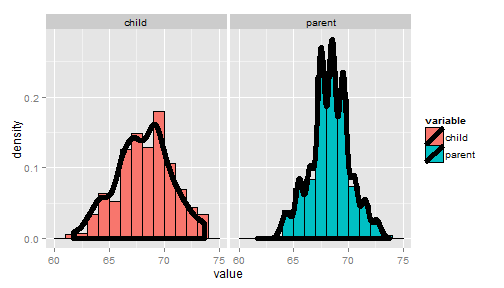
\includegraphics{LeanPub/images/galton-1.png}
\caption{Galton's Data}
\end{figure}

Using rStudio's \texttt{manipulate} package, you can try moving the
histogram around and see what value balances it out. Be sure to watch
the video to see this in action.

\vspace{1pc}

\verb;Using manipulate to explore the mean:;

\begin{Shaded}
\begin{Highlighting}[]
\KeywordTok{library}\NormalTok{(manipulate)}
\NormalTok{myHist <-}\StringTok{ }\NormalTok{function(mu)\{}
    \NormalTok{g <-}\StringTok{ }\KeywordTok{ggplot}\NormalTok{(galton, }\KeywordTok{aes}\NormalTok{(}\DataTypeTok{x =} \NormalTok{child))}
    \NormalTok{g <-}\StringTok{ }\NormalTok{g +}\StringTok{ }\KeywordTok{geom_histogram}\NormalTok{(}\DataTypeTok{fill =} \StringTok{"salmon"}\NormalTok{,}
      \DataTypeTok{binwidth=}\DecValTok{1}\NormalTok{, }\KeywordTok{aes}\NormalTok{(}\DataTypeTok{y =} \NormalTok{..density..), }\DataTypeTok{color =} \StringTok{"black"}\NormalTok{)}
    \NormalTok{g <-}\StringTok{ }\NormalTok{g +}\StringTok{ }\KeywordTok{geom_density}\NormalTok{(}\DataTypeTok{size =} \DecValTok{2}\NormalTok{)}
    \NormalTok{g <-}\StringTok{ }\NormalTok{g +}\StringTok{ }\KeywordTok{geom_vline}\NormalTok{(}\DataTypeTok{xintercept =} \NormalTok{mu, }\DataTypeTok{size =} \DecValTok{2}\NormalTok{)}
    \NormalTok{mse <-}\StringTok{ }\KeywordTok{round}\NormalTok{(}\KeywordTok{mean}\NormalTok{((galton$child -}\StringTok{ }\NormalTok{mu)^}\DecValTok{2}\NormalTok{), }\DecValTok{3}\NormalTok{)  }
    \NormalTok{g <-}\StringTok{ }\NormalTok{g +}\StringTok{ }\KeywordTok{labs}\NormalTok{(}\DataTypeTok{title =} \KeywordTok{paste}\NormalTok{(}\StringTok{'mu = '}\NormalTok{, mu, }\StringTok{' MSE = '}\NormalTok{, mse))}
    \NormalTok{g}
\NormalTok{\}}
\KeywordTok{manipulate}\NormalTok{(}\KeywordTok{myHist}\NormalTok{(mu),}
           \DataTypeTok{mu =} \KeywordTok{slider}\NormalTok{(}\DecValTok{62}\NormalTok{, }\DecValTok{74}\NormalTok{, }\DataTypeTok{step =} \FloatTok{0.5}\NormalTok{, }\DataTypeTok{initial=}\KeywordTok{mean}\NormalTok{(galton$child)))}
\end{Highlighting}
\end{Shaded}

Going through this exercise, you find that the point that balances out
the histogram is the empirical mean. (Note there's a small distinction
here that comes about from rounding with the histogram bar widths, but
ignore that for the time being.) If the bars of the histogram are from
the observed data, the point that balances it out is the empirical mean;
if the bars are the true population probabilities (which we don't know
of course) then the point is the population mean. Let's now go through
some examples of mathematically calculating the population mean.

\subsubsection{The center of mass is the empirical
mean}\label{the-center-of-mass-is-the-empirical-mean}

\begin{figure}[htbp]
\centering
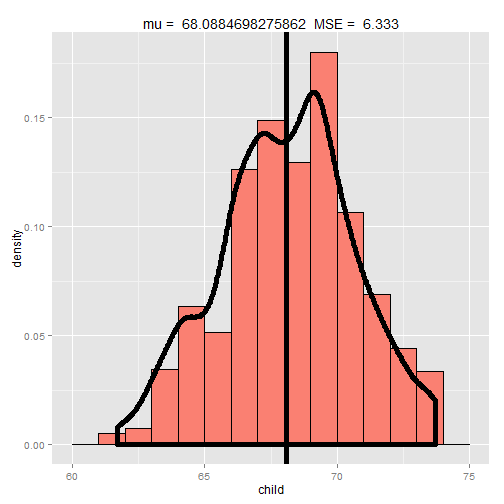
\includegraphics{LeanPub/images/lsm-1.png}
\caption{Histogram illustration}
\end{figure}

\subsubsection{Example of a population mean, a fair
coin}\label{example-of-a-population-mean-a-fair-coin}

\href{http://youtu.be/F4XMuD_axN8?list=PLpl-gQkQivXiBmGyzLrUjzsblmQsLtkzJ}{Watch
the video before beginning here.}

Suppose a coin is flipped and $X$ is declared 0 or 1 corresponding to a
head or a tail, respectively. What is the expected value of $X$?

\[
E[X] = .5 \times 0 + .5 \times 1 = .5
\]

Note, if thought about geometrically, this answer is obvious; if two
equal weights are spaced at 0 and 1, the center of mass will be 0.5.

\begin{figure}[htbp]
\centering
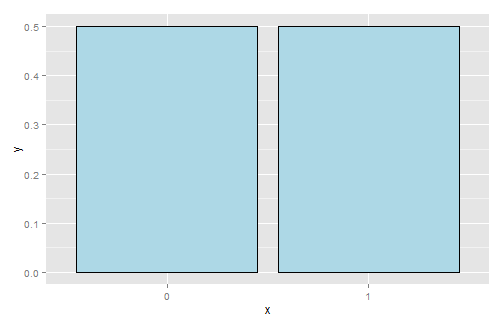
\includegraphics{LeanPub/images/fairCoin-1.png}
\caption{Fair coin mass function}
\end{figure}

\subsubsection{What about a biased
coin?}\label{what-about-a-biased-coin}

Suppose that a random variable, $X$ , is so that $P(X=1) = p$ and
$P(X=0) = (1 - p)$ (This is a biased coin when $p\neq 0.5$.) What is its
expected value?

\[
E[X] = 0 * (1 - p) + 1 * p = p
\]

Notice that the expected value isn't a value that the coin can take in
the same way that the sample proportion of heads will also likely be
neither 0 nor 1.

This coin example is not exactly trivial as it serves as the basis for a
random sample of any population for a binary trait. So, we might model
the answer from an election polling question as if it were a coin flip.

\subsubsection{Example Die Roll}\label{example-die-roll}

Suppose that a die is rolled and $X$ is the number face up. What is the
expected value of $X$?

\[
E[X] = 1 \times \frac{1}{6} + 2 \times \frac{1}{6} +
3 \times \frac{1}{6} + 4 \times \frac{1}{6} +
5 \times \frac{1}{6} + 6 \times \frac{1}{6} = 3.5
\]

Again, the geometric argument makes this answer obvious without
calculation.

\begin{figure}[htbp]
\centering
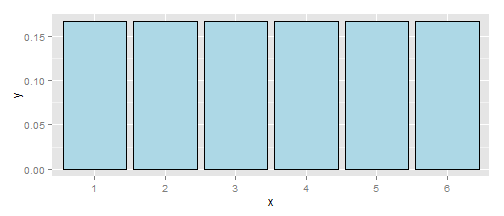
\includegraphics{LeanPub/images/die-1.png}
\caption{Bar graph of die probabilities}
\end{figure}

\subsection{Continuous random
variables}\label{continuous-random-variables}

\href{http://youtu.be/YS5EIKsamXI?list=PLpl-gQkQivXiBmGyzLrUjzsblmQsLtkzJ}{Watch
this video before beginning.}

For a continuous random variable, $X$, with density, $f$, the expected
value is again exactly the center of mass of the density. Think of it
like cutting the continuous density out of a thick piece of wood and
trying to find the point where it balances out.

\subsubsection{Example}\label{example-7}

Consider a density where $f(x) = 1$ for $x$ between zero and one.
Suppose that $X$ follows this density; what is its expected value?

\begin{figure}[htbp]
\centering
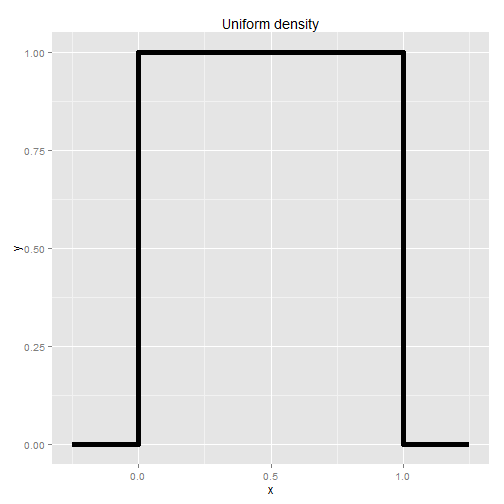
\includegraphics{LeanPub/images/uniform-1.png}
\caption{Uniform Density}
\end{figure}

The answer is clear since the density looks like a box, it would balance
out exactly in the middle, 0.5.

\subsubsection{Facts about expected
values}\label{facts-about-expected-values}

Recall that expected values are properties of population distributions.
The expected value, or mean, height is the center of the population
density of heights.

Of course, the average of ten randomly sampled people's height is itself
a random variable, in the same way that the average of ten die rolls is
itself a random number. Thus, the distribution of heights gives rise to
the distribution of averages of ten heights in the same way that
distribution associated with a die roll gives rise to the distribution
of the average of ten dice.

An important question to ask is: ``What does the distribution of
averages look like?''. This question is important, since it tells us
things about averages, the best way to estimate the population mean,
when we only get to observe one average.

Consider the die rolls again. If wanted to know the distribution of
averages of 100 die rolls, you could (at least in principle) roll 100
dice, take the average and repeat that process. Imagine, if you could
only roll the 100 dice once. Then we would have direct information about
the distribution of die rolls (since we have 100 of them), but we
wouldn't have any direct information about the distribution of the
average of 100 die rolls, since we only observed one average.

Fortunately, the mathematics tells us about that distribution. Notably,
it's centered at the same spot as the original distribution! Thus, the
distribution of the estimator (the sample mean) is centered at the
distribution of what it's estimating (the population mean). When the
expected value of an estimator is what its trying to estimate, we say
that the estimator is \textbf{unbiased}.

Let's go through several simulation experiments to see this more fully.

\subsection{Simulation experiments}\label{simulation-experiments}

\subsubsection{Standard normals}\label{standard-normals}

Consider simulating a lot of standard normals and plotting a histogram
(the blue density). Now consider simulating lots of averages of 10
standard normals and plotting their histogram (the salmon colored
density). Notice that they're centered in the same spot! It's also more
concentrated around that point. (We'll discuss that more in the next
lectures).

\begin{figure}[htbp]
\centering
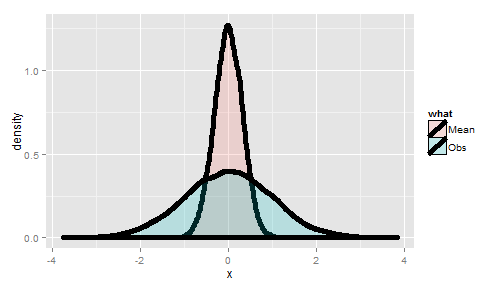
\includegraphics{LeanPub/images/normalSimulationMean-1.png}
\caption{Simulation of normals}
\end{figure}

\subsubsection{Averages of x die rolls}\label{averages-of-x-die-rolls}

Consider rolling a die a lot of times and taking a histogram of the
results, that's the left most plot. The bars are equally distributed at
the six possible outcomes and thus the histogram is centered around 3.5.
Now consider simulating lots of averages of 2 dice. Its histogram is
also centered at 3.5. So is it for 3 and 4. Notice also the distribution
gets increasing Gaussian looking (like a bell curve) and increasingly
concentrated around 3.5.

\begin{figure}[htbp]
\centering
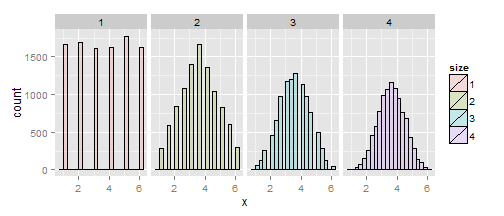
\includegraphics{LeanPub/images/dieRollSimulationMean-1.png}
\caption{Simulation of die rolls}
\end{figure}

\subsubsection{Averages of x coin flips}\label{averages-of-x-coin-flips}

For the coin flip simulation exactly the same occurs. All of the
distributions are centered around 0.5.

\begin{figure}[htbp]
\centering
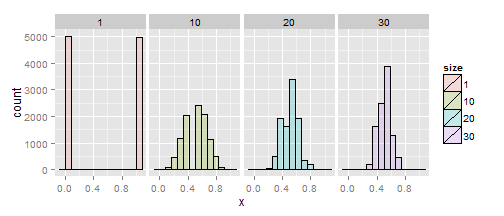
\includegraphics{LeanPub/images/coinFlipSimulationMean-1.png}
\caption{Simulation of coin flips}
\end{figure}

\subsection{Summary notes}\label{summary-notes-1}

\begin{itemize}
\itemsep1pt\parskip0pt\parsep0pt
\item
  Expected values are properties of distributions.
\item
  The population mean is the center of mass of population.
\item
  The sample mean is the center of mass of the observed data.
\item
  The sample mean is an estimate of the population mean.
\item
  The sample mean is unbiased: the population mean of its distribution
  is the mean that it's trying to estimate.
\item
  The more data that goes into the sample mean, the more. concentrated
  its density / mass function is around the population mean.
\end{itemize}

\subsection{Exercises}\label{exercises-3}

\begin{enumerate}
\def\labelenumi{\arabic{enumi}.}
\itemsep1pt\parskip0pt\parsep0pt
\item
  A standard die takes the values 1, 2, 3, 4, 5, 6 with equal
  probability. What is the expected value?
\item
  Consider a density that is uniform from -1 to 1. (I.e. has height
  equal to 1/2 and looks like a box starting at -1 and ending at 1).
  What is the mean of this distribution?
\item
  If a population has mean $\mu$, what is the mean of the distribution
  of averages of 20 observations from this distribution?
\item
  You are playing a game with a friend where you flip a coin and if it
  comes up heads you give her $X$ dollars and if it comes up tails she
  gives you $Y$ dollars. The odds that the coin is heads is $d$. What is
  your expected earnings?
  \href{http://youtu.be/5J88Zq0q81o?list=PLpl-gQkQivXhHOcVeU3bSJg78zaDYbP9L}{Watch
  a video of the solution to this problem} and
  \href{http://bcaffo.github.io/courses/06_StatisticalInference/homework/hw1.html\#5}{look
  at the problem and the solution here.}.
\item
  If you roll ten standard dice, take their average, then repeat this
  process over and over and construct a histogram what would it be
  centered at?
  \href{https://www.youtube.com/watch?v=ia3n2URiJaw\&index=16\&list=PLpl-gQkQivXhHOcVeU3bSJg78zaDYbP9L}{Watch
  a video solution here} and
  \href{http://bcaffo.github.io/courses/06_StatisticalInference/homework/hw2.html\#11}{see
  the original problem here}.
\end{enumerate}

\newpage

\section{Variation}\label{variation}

\subsection{The variance}\label{the-variance}

\href{http://youtu.be/oLQVU-VRiHo?list=PLpl-gQkQivXiBmGyzLrUjzsblmQsLtkzJ}{Watch
this video before beginning.}

Recall that the mean of distribution was a measure of its center. The
variance, on the other hand, is a measure of \emph{spread}. To get a
sense, the plot below shows a series of increasing variances.

\begin{figure}[htbp]
\centering
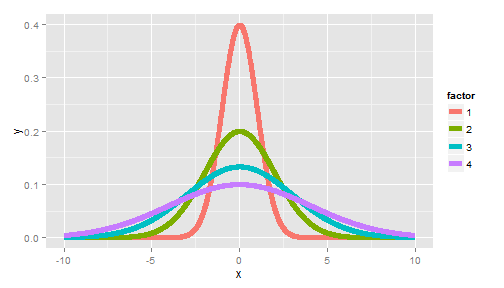
\includegraphics{LeanPub/images/normalVariances2-1.png}
\caption{Distributions with increasing variance}
\end{figure}

We saw another example of how variances changed in the last chapter when
we looked at the distribution of averages; they were always centered at
the same spot as the original distribution, but are less spread out.
Thus, it is less likely for sample means to be far away from the
population mean than it is for individual observations. (This is why the
sample mean is a better estimate than the population mean.)

If $X$ is a random variable with mean $\mu$, the variance of $X$ is
defined as

\[
Var(X) = E[(X - \mu)^2] = E[X^2] - E[X]^2.
\]

The rightmost equation is the shortcut formula that is almost always
used for calculating variances in practice.\\Thus the variance is the
expected (squared) distance from the mean. Densities with a higher
variance are more spread out than densities with a lower variance. The
square root of the variance is called the \textbf{standard deviation}.
The main benefit of working with standard deviations is that they have
the same units as the data, whereas the variance has the units squared.

In this class, we'll only cover a few basic examples for calculating a
variance. Otherwise, we're going to use the ideas without the formalism.
Also remember, what we're talking about is the population variance. It
measures how spread out the population of interest is, unlike the sample
variance which measures how spread out the observed data are. Just like
the sample mean estimates the population mean, the sample variance will
estimate the population variance.

\subsubsection{Example}\label{example-8}

What's the variance from the result of a toss of a die? First recall
that $E[X] = 3.5$, as we discussed in the previous lecture. Then let's
calculate the other bit of information that we need, $E[X^2]$.

\[E[X^2] = 1 ^ 2 \times \frac{1}{6} + 2 ^ 2 \times \frac{1}{6} + 3 ^ 2 \times \frac{1}{6} + 4 ^ 2 \times \frac{1}{6} + 5 ^ 2 \times \frac{1}{6} + 6 ^ 2 \times \frac{1}{6} = 15.17\]

Thus now we can calculate the variance as:

\[Var(X) = E[X^2] - E[X]^2 \approx 2.92.\]

\subsubsection{Example}\label{example-9}

What's the variance from the result of the toss of a (potentially
biased) coin with probability of heads (1) of $p$? First recall that
$E[X] = 0 \times (1 - p) + 1 \times p = p.$ Secondly, recall that since
$X$ is either 0 or 1, $X^2 = X$. So we know that:

\[E[X^2] = E[X] = p.\]

Thus we can now calculate the variance of a coin flip as
$Var(X) = E[X^2] - E[X]^2 = p - p^2 = p(1 - p).$ This is a well known
formula, so it's worth committing to memory. It's interesting to note
that this function is maximized at $p = 0.5$. The plot below shows this
by plotting $p(1-p)$ by $p$.

\vspace{1pc}

\verb;Plotting the binomial variance:;

\begin{Shaded}
\begin{Highlighting}[]
\NormalTok{p =}\StringTok{ }\KeywordTok{seq}\NormalTok{(}\DecValTok{0} \NormalTok{, }\DecValTok{1}\NormalTok{, }\DataTypeTok{length =} \DecValTok{1000}\NormalTok{)}
\NormalTok{y =}\StringTok{ }\NormalTok{p *}\StringTok{ }\NormalTok{(}\DecValTok{1} \NormalTok{-}\StringTok{ }\NormalTok{p)}
\KeywordTok{plot}\NormalTok{(p, y, }\DataTypeTok{type =} \StringTok{"l"}\NormalTok{, }\DataTypeTok{lwd =} \DecValTok{3}\NormalTok{, }\DataTypeTok{frame =} \OtherTok{FALSE}\NormalTok{)}
\end{Highlighting}
\end{Shaded}

\begin{figure}[htbp]
\centering
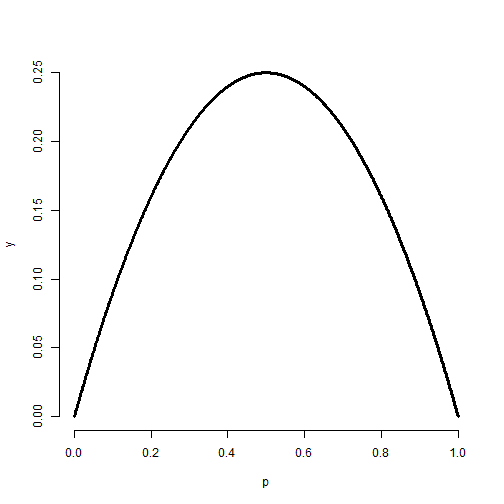
\includegraphics{LeanPub/images/binomialVariance-1.png}
\caption{Plot of the binomial variance}
\end{figure}

\subsection{The sample variance}\label{the-sample-variance}

The sample variance is the estimator of the population variance. Recall
that the population variance is the expected squared deviation around
the population mean. The sample variance is (almost) the average squared
deviation of observations around the sample mean. It is given by

\[
S^2 = \frac{\sum_{i=1} (X_i - \bar X)^2}{n-1}
\]

The sample standard deviation is the square root of the sample variance.
Note again that the sample variance is almost, but not quite, the
average squared deviation from the sample mean since we divide by $n-1$
instead of $n$. Why do we do this you might ask? To answer that question
we have to think in the terms of simulations. Remember that the sample
variance is a random variable, thus it has a distribution and that
distribution has an associated population mean. That mean is the
population variance that we're trying to estimate if we divide by
$(n-1)$ rather than $n$.

It is also nice that as we collect more data the distribution of the
sample variance gets more concentrated around the population variance
that it's estimating.

\subsection{Simulation experiments}\label{simulation-experiments-1}

\href{http://youtu.be/uPjHB9JjGKI?list=PLpl-gQkQivXiBmGyzLrUjzsblmQsLtkzJ}{Watch
this video before beginning.}

\subsubsection{Simulating from a population with variance
1}\label{simulating-from-a-population-with-variance-1}

Let's try simulating collections of standard normals and taking the
variance. If we repeat this over and over, we get a sense of the
distribution of sample variances variances.

\begin{figure}[htbp]
\centering
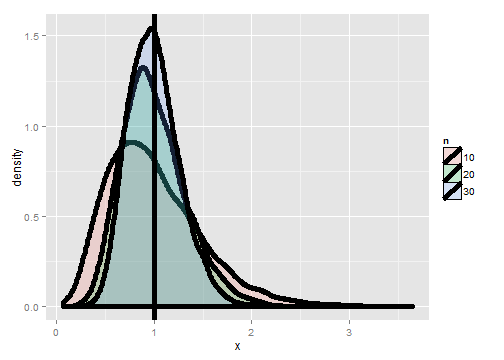
\includegraphics{LeanPub/images/normalVariances-1.png}
\caption{Simulation of variances of samples of standard normals}
\end{figure}

Notice that these histograms are always centered in the same spot, 1. In
other words, the sample variance is an unbiased estimate of the
population variances. Notice also that they get more concentrated around
the 1 as more data goes into them. Thus, sample variances comprised of
more observations are less variable than sample variances comprised of
fewer.

\subsubsection{Variances of x die rolls}\label{variances-of-x-die-rolls}

Let's try the same thing, now only with die rolls instead of simulating
standard normals. In this experiment, we simulated samples of die rolls,
took the variance and then repeated that process over and over. What is
plotted are histograms of the collections of sample variances.

\begin{figure}[htbp]
\centering
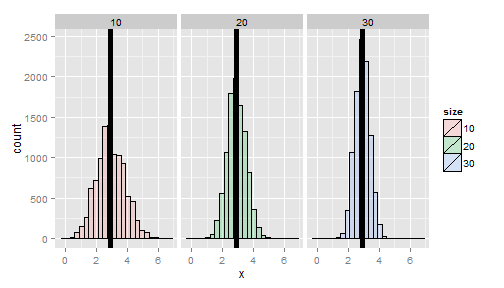
\includegraphics{LeanPub/images/dieVariances-1.png}
\caption{Simulated distributions of variances of dice}
\end{figure}

Recall that we calculated the variance of a die roll as 2.92 earlier on
in this chapter. Notice each of the histograms are centered there. In
addition, they get more concentrated around 2.92 as more the variances
are comprised of more dice.

\subsection{The standard error of the
mean}\label{the-standard-error-of-the-mean}

At last, we finally get to a perhaps very surprising (and useful) fact:
how to estimate the variability of the mean of a sample, when we only
get to observe one realization. Recall that the average of random sample
from a population is itself a random variable having a distribution,
which in simulation settings we can explore by repeated sampling
averages. We know that this distribution is centered around the
population mean, $E[\bar X] = \mu$. We also know the variance of the
distribution of means of random samples.

The variance of the sample mean is: $Var(\bar X) = \sigma^2 / n$ where
$\sigma^2$ is the variance of the population being sampled from.

This is very useful, since we don't have repeat sample means to get its
variance directly using the data. We already know a good estimate of
$\sigma^2$ via the sample variance. So, we can get a good estimate of
the variability of the mean, even though we only get to observe 1 mean.

Notice also this explains why in all of our simulation experiments the
variance of the sample mean kept getting smaller as the sample size
increased. This is because of the square root of the sample size in the
denominator.

Often we take the square root of the variance of the mean to get the
standard deviation of the mean. We call the standard deviation of a
statistic its standard error.

\subsubsection{Summary notes}\label{summary-notes-2}

\begin{itemize}
\itemsep1pt\parskip0pt\parsep0pt
\item
  The sample variance, $S^2$, estimates the population variance,
  $\sigma^2$.
\item
  The distribution of the sample variance is centered around $\sigma^2$.
\item
  The variance of the sample mean is $\sigma^2 / n$.
\item
  Its logical estimate is $s^2 / n$.
\item
  The logical estimate of the standard error is $S / \sqrt{n}$.
\item
  $S$, the standard deviation, talks about how variable the population
  is.
\item
  $S/\sqrt{n}$, the standard error, talks about how variable averages of
  random samples of size $n$ from the population are.
\end{itemize}

\subsubsection{Simulation example 1: standard
normals}\label{simulation-example-1-standard-normals}

\href{http://youtu.be/uPjHB9JjGKI?list=PLpl-gQkQivXiBmGyzLrUjzsblmQsLtkzJ}{Watch
this video before beginning.}

Standard normals have variance 1. Let's try sampling means of $n$
standard normals. If our theory is correct, they should have standard
deviation $1/\sqrt{n}$

\vspace{1pc}

\verb;Simulating means of random normals:;

\begin{Shaded}
\begin{Highlighting}[]
\NormalTok{nosim <-}\StringTok{ }\DecValTok{1000}
\NormalTok{n <-}\StringTok{ }\DecValTok{10}
\NormalTok{## simulate nosim averages of 10 standard normals}
\KeywordTok{sd}\NormalTok{(}\KeywordTok{apply}\NormalTok{(}\KeywordTok{matrix}\NormalTok{(}\KeywordTok{rnorm}\NormalTok{(nosim *}\StringTok{ }\NormalTok{n), nosim), }\DecValTok{1}\NormalTok{, mean))}
\end{Highlighting}
\end{Shaded}

\begin{verbatim}
## [1] 0.313551
\end{verbatim}

\begin{Shaded}
\begin{Highlighting}[]
\NormalTok{## Let's check to make sure that this is sigma / sqrt(n)}
\DecValTok{1} \NormalTok{/}\StringTok{ }\KeywordTok{sqrt}\NormalTok{(n)}
\end{Highlighting}
\end{Shaded}

\begin{verbatim}
## [1] 0.3162278
\end{verbatim}

So, in this simulation, we simulated 1000 means of 10 standard normals.
Our theory says the standard deviation of averages of 10 standard
normals must be $1/\sqrt{n}$. Taking the standard deviation of the 10000
means yields nearly exactly that. (Note that it's only close, 0.3156
versus 0.31632. To get it to be exact, we'd have to simulate infinitely
many means.)

\subsubsection{Simulation example 2: uniform
density}\label{simulation-example-2-uniform-density}

Standard uniforms have variance $1/12$. Our theory mandates that means
of random samples of $n$ uniforms have sd $1/\sqrt{12 \times n}$. Let's
try it with a simulation.

\vspace{1pc}

\verb;Simulating means of uniforms:;

\begin{Shaded}
\begin{Highlighting}[]
\NormalTok{nosim <-}\StringTok{ }\DecValTok{1000}
\NormalTok{n <-}\StringTok{ }\DecValTok{10}
\KeywordTok{sd}\NormalTok{(}\KeywordTok{apply}\NormalTok{(}\KeywordTok{matrix}\NormalTok{(}\KeywordTok{runif}\NormalTok{(nosim *}\StringTok{ }\NormalTok{n), nosim), }\DecValTok{1}\NormalTok{, mean))}
\end{Highlighting}
\end{Shaded}

\begin{verbatim}
## [1] 0.08856019
\end{verbatim}

\begin{Shaded}
\begin{Highlighting}[]
\DecValTok{1} \NormalTok{/}\StringTok{ }\KeywordTok{sqrt}\NormalTok{(}\DecValTok{12} \NormalTok{*}\StringTok{ }\NormalTok{n)}
\end{Highlighting}
\end{Shaded}

\begin{verbatim}
## [1] 0.09128709
\end{verbatim}

\subsubsection{Simulation example 3:
Poisson}\label{simulation-example-3-poisson}

Poisson(4) random variables have variance $4$. Thus means of random
samples of $n$ Poisson(4) should have standard deviation $2/\sqrt{n}$.
Again let's try it out.

\vspace{1pc}

\verb;Simulating means of Poisson variates:;

\begin{Shaded}
\begin{Highlighting}[]
\NormalTok{nosim <-}\StringTok{ }\DecValTok{1000}
\NormalTok{n <-}\StringTok{ }\DecValTok{10}
\KeywordTok{sd}\NormalTok{(}\KeywordTok{apply}\NormalTok{(}\KeywordTok{matrix}\NormalTok{(}\KeywordTok{rpois}\NormalTok{(nosim *}\StringTok{ }\NormalTok{n, }\DecValTok{4}\NormalTok{), nosim), }\DecValTok{1}\NormalTok{, mean))}
\end{Highlighting}
\end{Shaded}

\begin{verbatim}
## [1] 0.6336028
\end{verbatim}

\begin{Shaded}
\begin{Highlighting}[]
\DecValTok{2} \NormalTok{/}\StringTok{ }\KeywordTok{sqrt}\NormalTok{(n)}
\end{Highlighting}
\end{Shaded}

\begin{verbatim}
## [1] 0.6324555
\end{verbatim}

\subsubsection{Simulation example 4: coin
flips}\label{simulation-example-4-coin-flips}

Our last example is an important one. Recall that the variance of a coin
flip is $p (1 - p)$. Therefore the standard deviation of the average of
$n$ coin flips should be $\sqrt{\frac{p(1-p)}{n}}$.

Let's just do the simulation with a fair coin. Such coin flips have
variance 0.25. Thus means of random samples of $n$ coin flips have sd
$1 / (2 \sqrt{n})$. Let's try it.

\vspace{1pc}

\verb;Simulating means of coin flips:;

\begin{Shaded}
\begin{Highlighting}[]
\NormalTok{nosim <-}\StringTok{ }\DecValTok{1000}
\NormalTok{n <-}\StringTok{ }\DecValTok{10}
\KeywordTok{sd}\NormalTok{(}\KeywordTok{apply}\NormalTok{(}\KeywordTok{matrix}\NormalTok{(}\KeywordTok{sample}\NormalTok{(}\DecValTok{0} \NormalTok{:}\StringTok{ }\DecValTok{1}\NormalTok{, nosim *}\StringTok{ }\NormalTok{n, }\DataTypeTok{replace =} \OtherTok{TRUE}\NormalTok{),}
                \NormalTok{nosim), }\DecValTok{1}\NormalTok{, mean))}
\end{Highlighting}
\end{Shaded}

\begin{verbatim}
## [1] 0.15867
\end{verbatim}

\begin{Shaded}
\begin{Highlighting}[]
\DecValTok{1} \NormalTok{/}\StringTok{ }\NormalTok{(}\DecValTok{2} \NormalTok{*}\StringTok{ }\KeywordTok{sqrt}\NormalTok{(n))}
\end{Highlighting}
\end{Shaded}

\begin{verbatim}
## [1] 0.1581139
\end{verbatim}

\subsection{Data example}\label{data-example}

\href{http://youtu.be/Lm2DMVyZVxk?list=PLpl-gQkQivXiBmGyzLrUjzsblmQsLtkzJ}{Watch
this before beginning.}

Now let's work through a data example to show how the standard error of
the mean is used in practice. We'll use the \texttt{father.son} height
data from Francis Galton.

\vspace{1pc}

\verb;Loading the data:;

\begin{Shaded}
\begin{Highlighting}[]
\KeywordTok{library}\NormalTok{(UsingR); }\KeywordTok{data}\NormalTok{(father.son);}
\NormalTok{x <-}\StringTok{ }\NormalTok{father.son$sheight}
\NormalTok{n<-}\KeywordTok{length}\NormalTok{(x)}
\end{Highlighting}
\end{Shaded}

Here's a histogram of the sons' heights from the dataset. Let' calculate
different variances and interpret them in this context.

\begin{figure}[htbp]
\centering
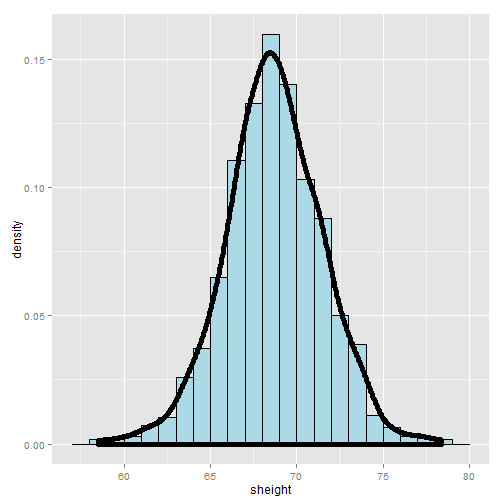
\includegraphics{LeanPub/images/fatherSon-1.png}
\caption{Histogram of the sons' heights}
\end{figure}

\begin{Shaded}
\begin{Highlighting}[]
\KeywordTok{round}\NormalTok{(}\KeywordTok{c}\NormalTok{(}\KeywordTok{var}\NormalTok{(x), }\KeywordTok{var}\NormalTok{(x) /}\StringTok{ }\NormalTok{n, }\KeywordTok{sd}\NormalTok{(x), }\KeywordTok{sd}\NormalTok{(x) /}\StringTok{ }\KeywordTok{sqrt}\NormalTok{(n)),}\DecValTok{2}\NormalTok{)}
\end{Highlighting}
\end{Shaded}

\begin{verbatim}
## [1] 7.92 0.01 2.81 0.09
\end{verbatim}

The first number, 7.92, and its square root, 2.81, are the estimated
variance and standard deviation of the sons' heights. Therefore, 7.92
tells us exactly how variable sons' heights were in the data and
estimates how variable sons' heights are in the population. In contrast
0.01, and the square root 0.09, estimate how variable averages of $n$
sons' heights are.

Therefore, the smaller numbers discuss the precision of our estimate of
the mean of sons' heights. The larger numbers discuss how variable sons'
heights are in general.

\subsection{Summary notes}\label{summary-notes-3}

\begin{itemize}
\itemsep1pt\parskip0pt\parsep0pt
\item
  The sample variance estimates the population variance.
\item
  The distribution of the sample variance is centered at what its
  estimating.
\item
  It gets more concentrated around the population variance with larger
  sample sizes.
\item
  The variance of the sample mean is the population variance divided by
  $n$.
\item
  The square root is the standard error.
\item
  It turns out that we can say a lot about the distribution of averages
  from random samples, even though we only get one to look at in a given
  data set.
\end{itemize}

\subsection{Exercises}\label{exercises-4}

\begin{enumerate}
\def\labelenumi{\arabic{enumi}.}
\itemsep1pt\parskip0pt\parsep0pt
\item
  If I have a random sample from a population, the sample variance is an
  estimate of?
\end{enumerate}

\begin{itemize}
\itemsep1pt\parskip0pt\parsep0pt
\item
  The population standard deviation.
\item
  The population variance.
\item
  The sample variance.
\item
  The sample standard deviation.
\end{itemize}

\begin{enumerate}
\def\labelenumi{\arabic{enumi}.}
\setcounter{enumi}{1}
\itemsep1pt\parskip0pt\parsep0pt
\item
  The distribution of the sample variance of a random sample from a
  population is centered at what?
\end{enumerate}

\begin{itemize}
\itemsep1pt\parskip0pt\parsep0pt
\item
  The population variance.
\item
  The population mean.
\end{itemize}

\begin{enumerate}
\def\labelenumi{\arabic{enumi}.}
\setcounter{enumi}{2}
\itemsep1pt\parskip0pt\parsep0pt
\item
  I keep drawing samples of size $n$ from a population with variance
  $\sigma^2$ and taking their average. I do this thousands of times. If
  I were to take the variance of the collection of averages, about what
  would it be?
\item
  You get a random sample of $n$ observations from a population and take
  their average. You would like to estimate the variability of averages
  of $n$ observations from this population to better understand how
  precise of an estimate it is. Do you need to repeated collect averages
  to do this?
\end{enumerate}

\begin{itemize}
\itemsep1pt\parskip0pt\parsep0pt
\item
  No, we can multiply our estimate of the population variance by $1/n$
  to get a good estimate of the variability of the average.
\item
  Yes, you have to get repeat averages.
\end{itemize}

\begin{enumerate}
\def\labelenumi{\arabic{enumi}.}
\setcounter{enumi}{4}
\itemsep1pt\parskip0pt\parsep0pt
\item
  A random variable takes the value -4 with probability .2 and 1 with
  probability .8. What is the variance of this random variable?
  \href{http://youtu.be/Em-xJeQO1rc?list=PLpl-gQkQivXhHOcVeU3bSJg78zaDYbP9L}{Watch
  a video solution to this problem.} and
  \href{http://bcaffo.github.io/courses/06_StatisticalInference/homework/hw1.html\#6}{look
  at a version with a worked out solution.}
\item
  If $\bar X$ and $\bar Y$ are comprised of n iid random variables
  arising from distributions having means $\mu_x$ and $\mu_y$,
  respectively and common variance $\sigma^2$ what is the variance
  $\bar X - \bar Y$?
  \href{http://youtu.be/7zJhPzX6jns?list=PLpl-gQkQivXhHOcVeU3bSJg78zaDYbP9L}{Watch
  a video solution to this problem here} and
  \href{http://bcaffo.github.io/courses/06_StatisticalInference/homework/hw1.html\#7}{see
  a typed up solution here}
\item
  Let $X$ be a random variable having standard deviation $\sigma$. What
  can be said about the variance of $X /\sigma$?
  \href{http://youtu.be/0WUj18_BUPA?list=PLpl-gQkQivXhHOcVeU3bSJg78zaDYbP9L}{Watch
  a video solution to this problem here} and
  \href{http://bcaffo.github.io/courses/06_StatisticalInference/homework/hw1.html\#8}{typed
  up solutions here}.
\item
  Consider the following pmf given in R by the code
  \texttt{p \textless{}- c(.1, .2, .3, .4)} and 'x \textless{}- 2 : 5`.
  What is the variance?
  \href{http://youtu.be/HSn8n4DsGSg?list=PLpl-gQkQivXhHOcVeU3bSJg78zaDYbP9L}{Watch
  a video solution to this problem here} and
  \href{http://bcaffo.github.io/courses/06_StatisticalInference/homework/hw1.html\#10}{here
  is the problem worked out}.
\item
  If you roll ten standard dice, take their average, then repeat this
  process over and over and construct a histogram, what would be its
  variance expressed to 3 decimal places?
  \href{https://www.youtube.com/watch?v=MLfo9zz1zX4\&list=PLpl-gQkQivXhHOcVeU3bSJg78zaDYbP9L\&index=17}{Watch
  a video solution here} and
  \href{http://bcaffo.github.io/courses/06_StatisticalInference/homework/hw2.html\#12}{see
  the text here}.
\end{enumerate}

\newpage

\section{Some common distributions}\label{some-common-distributions}

\subsection{The Bernoulli
distribution}\label{the-bernoulli-distribution}

The \textbf{Bernoulli distribution} arises as the result of a binary
outcome, such as a coin flip. Thus, Bernoulli random variables take
(only) the values 1 and 0 with probabilities of (say) $p$ and $1-p$,
respectively. Recall that the PMF for a Bernoulli random variable $X$ is
$P(X = x) =  p^x (1 - p)^{1 - x}$.

The mean of a Bernoulli random variable is $p$ and the variance is
$p(1 - p)$. If we let $X$ be a Bernoulli random variable, it is typical
to call $X=1$ as a ``success'' and $X=0$ as a ``failure''.

If a random variable follows a Bernoulli distribution with success
probability $p$ we write that $X \sim$ Bernoulli$(p)$.

Bernoulli random variables are commonly used for modeling any binary
trait for a random sample. So, for example, in a random sample whether
or not a participant has high blood pressure would be reasonably modeled
as Bernoulli.

\subsection{Binomial trials}\label{binomial-trials}

The \textbf{binomial random variables} are obtained as the sum of iid
Bernoulli trials. So if a Bernoulli trial is the result of a coin flip,
a binomial random variable is the total number of heads.

To write it out as mathematics, let $X_1,\ldots,X_n$ be iid
Bernoulli$(p)$, then $X = \sum_{i=1}^n X_i$ is a binomial random
variable. We write out that $X \sim$ Binomial$(n,p)$. The binomial mass
function is

\[
P(X = x) =
\left(
\begin{array}{c}
  n \\ x
\end{array}
\right)
p^x(1 - p)^{n-x}
\]

where $x=0,\ldots,n$. Recall that the notation

\[
\left(
  \begin{array}{c} n \\ x \end{array}
\right) = \frac{n!}{x!(n-x)!}
\]

(read ``$n$ choose $x$'') counts the number of ways of selecting $x$
items out of $n$ without replacement disregarding the order of the
items. It turns out that $n$ choose 0, $n$ choose 1 and $n$ choose $n-1$
are all 1.

\subsubsection{Example}\label{example-10}

Suppose a friend has 8 children, $7$ of which are girls and none are
twins. If each gender has an independent $50$\% probability for each
birth, what's the probability of getting $7$ or more girls out of $8$
births?

\[
\left(
\begin{array}{c}
  8 \\ 7
\end{array}
\right) .5^{7}(1-.5)^{1}
+
\left(
\begin{array}{c}
  8 \\ 8
\end{array}
\right) .5^{8}(1-.5)^{0} \approx 0.04 .
\]

\vspace{1pc}

\verb;Simulating means of coin flips:;

\begin{Shaded}
\begin{Highlighting}[]
\KeywordTok{choose}\NormalTok{(}\DecValTok{8}\NormalTok{, }\DecValTok{7}\NormalTok{) *}\StringTok{ }\FloatTok{0.5}\NormalTok{^}\DecValTok{8} \NormalTok{+}\StringTok{ }\KeywordTok{choose}\NormalTok{(}\DecValTok{8}\NormalTok{, }\DecValTok{8}\NormalTok{) *}\StringTok{ }\FloatTok{0.5}\NormalTok{^}\DecValTok{8}
\end{Highlighting}
\end{Shaded}

\begin{verbatim}
## [1] 0.03515625
\end{verbatim}

\begin{Shaded}
\begin{Highlighting}[]
\KeywordTok{pbinom}\NormalTok{(}\DecValTok{6}\NormalTok{, }\DataTypeTok{size =} \DecValTok{8}\NormalTok{, }\DataTypeTok{prob =} \FloatTok{0.5}\NormalTok{, }\DataTypeTok{lower.tail =} \OtherTok{FALSE}\NormalTok{)}
\end{Highlighting}
\end{Shaded}

\begin{verbatim}
## [1] 0.03515625
\end{verbatim}

\subsection{The normal distribution}\label{the-normal-distribution}

\href{http://youtu.be/dUTWvKa0Leo?list=PLpl-gQkQivXiBmGyzLrUjzsblmQsLtkzJ}{Watch
this video before beginning}

The normal distribution is easily the handiest distribution in all of
statistics. It can be used in an endless variety of settings. Moreover,
as we'll see later on in the course, sample means follow normal
distributions for large sample sizes.

Remember the goal of probability modeling. We are assuming a probability
distribution for our population as a way of parsimoniously
characterizing it. In fact, the normal distribution only requires two
numbers to characterize it. Specifically, a random variable is said to
follow a \textbf{normal} or \textbf{Gaussian} distribution with mean
$\mu$ and variance $\sigma^2$ if the associated density is:

\[
 (2\pi \sigma^2)^{-1/2}e^{-(x - \mu)^2/2\sigma^2}.
\]

If $X$ is a RV with this density then $E[X] = \mu$ and
$Var(X) = \sigma^2$. That is, the normal distribution is characterized
by the mean and variance. We write $X\sim N(\mu, \sigma^2)$ to denote a
normal random variable. When $\mu = 0$ and $\sigma = 1$ the resulting
distribution is called \textbf{the standard normal distribution}.
Standard normal RVs are often labeled $Z$

Consider an example, if we say that intelligence quotients are normally
distributed with a mean of 100 and a standard deviation of 15. Then, we
are saying that if we randomly sample a person from this population, the
probability that they have an IQ of say 120 or larger, is governed by a
normal distribution with a mean of 100 and a variance of $15^2$.

Taken another way, if we know that the population is normally
distributed then to estimate everything about the population, we need
only estimate the population mean and variance. (Estimated by the sample
mean and the sample variance.)

\subsubsection{Reference quantiles for the standard
normal}\label{reference-quantiles-for-the-standard-normal}

The normal distribution is so important that it is useful to memorize
reference probabilities and quantiles. The image below shows reference
lines at 0, 1, 2 and 3 standard deviations above and below 0. This is
for the standard normal; however, all of the rules apply to non standard
normals as 0, 1, 2 and 3 standard deviations above and below $\mu$, the
population mean.

\begin{figure}[htbp]
\centering
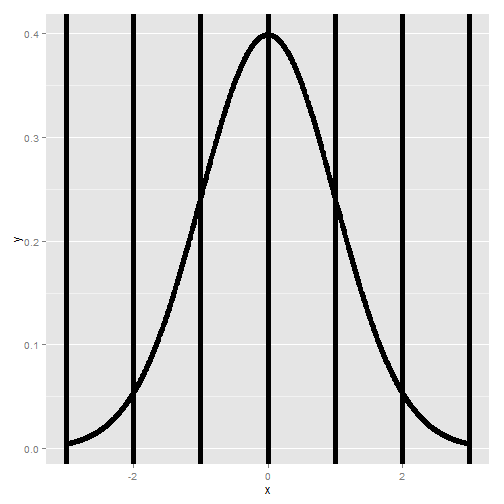
\includegraphics{LeanPub/images/normalReference-1.png}
\caption{Standard normal reference lines.}
\end{figure}

The most relevant probabilities are.

\begin{enumerate}
\def\labelenumi{\arabic{enumi}.}
\itemsep1pt\parskip0pt\parsep0pt
\item
  Approximately 68\%, 95\% and 99\% of the normal density lies within 1,
  2 and 3 standard deviations from the mean, respectively.
\item
  -1.28, -1.645, -1.96 and -2.33 are the $10^{th}$, $5^{th}$, $2.5^{th}$
  and $1^{st}$ percentiles of the standard normal distribution,
  respectively.
\item
  By symmetry, 1.28, 1.645, 1.96 and 2.33 are the $90^{th}$, $95^{th}$,
  $97.5^{th}$ and $99^{th}$ percentiles of the standard normal
  distribution, respectively.
\end{enumerate}

\subsubsection{Shifting and scaling
normals}\label{shifting-and-scaling-normals}

Since the normal distribution is characterized by only the mean and
variance, which are a shift and a scale, we can transform normal random
variables to be standard normals and vice versa. For example If
$X \sim N(\mu,\sigma^2)$ then:

\[Z = \frac{X -\mu}{\sigma} \sim N(0, 1).\]

If $Z$ is standard normal

\[X = \mu + \sigma Z \sim N(\mu, \sigma^2)\]

then $X$ is $X \sim N(\mu,\sigma^2)$. We can use these facts to answer
questions about non-standard normals by relating them back to the
standard normal.

\subsubsection{Example}\label{example-11}

What is the $95^{th}$ percentile of a $N(\mu, \sigma^2)$ distribution?
Quick answer in R \texttt{qnorm(.95, mean = mu, sd = sigma)}.
Alternatively, because we have the standard normal quantiles memorized,
and we know that 1.645 is its 95th percentile, the answer has to be
$\mu + \sigma 1.645$.

In general, $\mu + \sigma z_0$ where $z_0$ is the appropriate standard
normal quantile.

To put some context on our previous setting, population mean BMI for men
\href{http://www.ncbi.nlm.nih.gov/pubmed/23675464}{is reported as} 29
$kg/mg^2$ with a standard deviation of 4.73. Assuming normality of BMI,
what is the population $95^{th}$ percentile? The answer is then:

\[
29 + 4.73 \times 1.645 = 36.78.
\]

Or alternatively, we could simply type 36.7801577 in R.

Now let's reverse the process. Imaging asking what's the probability
that a randomly drawn subject from this population has a BMI less than
24.27? Notice that

\[
\frac{24.27 - 29}{4.73} = -1.
\]

Therefore, 24.27 is 1 standard deviation below the mean. We know that
16\% lies below or above 1 standard deviation from the mean. Thus 16\%
lies below. Alternatively, \texttt{pnorm(24.27, 29, 4.73)} yields the
result.

\subsubsection{Example}\label{example-12}

Assume that the number of daily ad clicks for a company is
(approximately) normally distributed with a mean of 1020 and a standard
deviation of 50. What's the probability of getting more than 1,160
clicks in a day? Notice that:

\[
\frac{1160 - 1020}{50} = 2.8
\]

Therefore, 1,160 is 2.8 standard deviations above the mean. We know from
our standard normal quantiles that the probability of being larger than
2 standard deviation is 2.5\% and 3 standard deviations is far in the
tail. Therefore, we know that the probability has to be smaller than
2.5\% and should be very small. We can obtain it exactly as 0.0025551
which is 0.3\%. Note that we can also obtain the probability as
0.0025551.

\subsubsection{Example}\label{example-13}

Consider the previous example again. What number of daily ad clicks
would represent the one where 75\% of days have fewer clicks (assuming
days are independent and identically distributed)? We can obtain this
as:

\vspace{1pc}

\verb;Finding a normal quantile:;

\begin{Shaded}
\begin{Highlighting}[]
\KeywordTok{qnorm}\NormalTok{(}\FloatTok{0.75}\NormalTok{, }\DataTypeTok{mean =} \DecValTok{1020}\NormalTok{, }\DataTypeTok{sd =} \DecValTok{50}\NormalTok{)}
\end{Highlighting}
\end{Shaded}

\begin{verbatim}
## [1] 1053.724
\end{verbatim}

\subsection{The Poisson distribution}\label{the-poisson-distribution}

\href{http://youtu.be/ZPLZg7qz4xE?list=PLpl-gQkQivXiBmGyzLrUjzsblmQsLtkzJ}{Watch
this video before beginning.}

The Poisson distribution is used to model counts. It is perhaps only
second to the normal distribution usefulness. In fact, the Bernoulli,
binomial and multinomial distributions can all be modeled by clever uses
of the Poisson.

The Poisson distribution is especially useful for modeling unbounded
counts or counts per unit of time (rates). Like the number of clicks on
advertisements, or the number of people who show up at a bus stop.
(While these are in principle bounded, it would be hard to actually put
an upper limit on it.) There is also a deep connection between the
Poisson distribution and popular models for so-called event-time data.
In addition, the Poisson distribution is the default model for so-called
contingency table data, which is simply tabulations of discrete
characteristics. Finally, when $n$ is large and $p$ is small, the
Poisson is an accurate approximation to the binomial distribution.

The Poisson mass function is:

\[
P(X = x; \lambda) = \frac{\lambda^x e^{-\lambda}}{x!}
\]

for $x=0,1,\ldots$. The mean of this distribution is $\lambda$. The
variance of this distribution is also $\lambda$. Notice that $x$ ranges
from 0 to $\infty$. Therefore, the Poisson distribution is especially
useful for modeling unbounded counts.

\subsubsection{Rates and Poisson random
variables}\label{rates-and-poisson-random-variables}

The Poisson distribution is useful for rates, counts that occur over
units of time. Specifically, if $X \sim Poisson(\lambda t)$ where
$\lambda = E[X / t]$ is the expected count per unit of time and $t$ is
the total monitoring time.

\subsubsection{Example}\label{example-14}

The number of people that show up at a bus stop is Poisson with a mean
of 2.5 per hour. If watching the bus stop for 4 hours, what is the
probability that $3$ or fewer people show up for the whole time?

\vspace{1pc}

\verb;Finding a Poisson quantile:;

\begin{Shaded}
\begin{Highlighting}[]
\KeywordTok{ppois}\NormalTok{(}\DecValTok{3}\NormalTok{, }\DataTypeTok{lambda =} \FloatTok{2.5} \NormalTok{*}\StringTok{ }\DecValTok{4}\NormalTok{)}
\end{Highlighting}
\end{Shaded}

\begin{verbatim}
## [1] 0.01033605
\end{verbatim}

Therefore, there is about a 1\% chance that 3 or fewer people show up.
Notice the multiplication by four in the function argument. Since lambda
is specified as events per \emph{hour} we have to multiply by four to
consider the number of events that occur in 4 hours.

\subsubsection{Poisson approximation to the
binomial}\label{poisson-approximation-to-the-binomial}

When $n$ is large and $p$ is small the Poisson distribution is an
accurate approximation to the binomial distribution. Formally, if
$X \sim \mbox{Binomial}(n, p)$ then $X$ is approximately Poisson where
$\lambda = n p$ provided that $n$ is large $p$ is small.

\paragraph{Example, Poisson approximation to the
binomial}\label{example-poisson-approximation-to-the-binomial}

We flip a coin with success probability 0.01 five hundred times. What's
the probability of 2 or fewer successes?

\vspace{1pc}

\verb;Aproximating a binomial quantile:;

\begin{Shaded}
\begin{Highlighting}[]
\KeywordTok{pbinom}\NormalTok{(}\DecValTok{2}\NormalTok{, }\DataTypeTok{size =} \DecValTok{500}\NormalTok{, }\DataTypeTok{prob =} \FloatTok{0.01}\NormalTok{)}
\end{Highlighting}
\end{Shaded}

\begin{verbatim}
## [1] 0.1233858
\end{verbatim}

\begin{Shaded}
\begin{Highlighting}[]
\KeywordTok{ppois}\NormalTok{(}\DecValTok{2}\NormalTok{, }\DataTypeTok{lambda =} \DecValTok{500} \NormalTok{*}\StringTok{ }\FloatTok{0.01}\NormalTok{)}
\end{Highlighting}
\end{Shaded}

\begin{verbatim}
## [1] 0.124652
\end{verbatim}

So we can see that the probabilities agree quite well. This
approximation is often done as the Poisson model is a more convenient
model in many respects.

\subsection{Exercises}\label{exercises-5}

\begin{enumerate}
\def\labelenumi{\arabic{enumi}.}
\itemsep1pt\parskip0pt\parsep0pt
\item
  Your friend claims that changing the font to comic sans will result in
  more ad revenue on your web sites. When presented in random order, 9
  pages out of 10 had more revenue when the font was set to comic sans.
  If it was really a coin flip for these 10 sites, what's the
  probability of getting 9 or 10 out of 10 with more revenue for the new
  font?
\item
  A software company is doing an analysis of documentation errors of
  their products. They sampled their very large codebase in chunks and
  found that the number of errors per chunk was approximately normally
  distributed with a mean of 11 errors and a standard deviation of 2.
  When randomly selecting a chunk from their codebase, whats the
  probability of fewer than 5 documentation errors?
\item
  The number of search entries entered at a web site is Poisson at a
  rate of 9 searches per minute. The site is monitored for 5 minutes.
  What is the probability of 40 or fewer searches in that time frame?
\item
  Suppose that the number of web hits to a particular site are
  approximately normally distributed with a mean of 100 hits per day and
  a standard deviation of 10 hits per day. What's the probability that a
  given day has fewer than 93 hits per day expressed as a percentage to
  the nearest percentage point?
  \href{https://www.youtube.com/watch?v=E-ancc7iTho\&index=10\&list=PLpl-gQkQivXhHOcVeU3bSJg78zaDYbP9L}{Watch
  a video solution} and
  \href{http://bcaffo.github.io/courses/06_StatisticalInference/homework/hw2.html\#4}{see
  the problem}.
\item
  Suppose that the number of web hits to a particular site are
  approximately normally distributed with a mean of 100 hits per day and
  a standard deviation of 10 hits per day. What number of web hits per
  day represents the number so that only 5\% of days have more hits?
  \href{https://www.youtube.com/watch?v=rv48_5C8gx4\&index=12\&list=PLpl-gQkQivXhHOcVeU3bSJg78zaDYbP9L}{Watch
  a video solution} and
  \href{http://bcaffo.github.io/courses/06_StatisticalInference/homework/hw2.html\#6}{see
  the problem and solution}.
\item
  Suppose that the number of web hits to a particular site are
  approximately normally distributed with a mean of 100 hits per day and
  a standard deviation of 10 hits per day. Imagine taking a random
  sample of 50 days. What number of web hits would be the point so that
  only 5\% of averages of 50 days of web traffic have more hits?
  \href{https://www.youtube.com/watch?v=c_B2AuOhdzg\&index=13\&list=PLpl-gQkQivXhHOcVeU3bSJg78zaDYbP9L}{Watch
  a video solution} and
  \href{http://bcaffo.github.io/courses/06_StatisticalInference/homework/hw2.html\#7}{see
  the problem and solution}.
\item
  You don't believe that your friend can discern good wine from cheap.
  Assuming that you're right, in a blind test where you randomize 6
  paired varieties (Merlot, Chianti, \ldots{}) of cheap and expensive
  wines. What is the change that she gets 5 or 6 right?
  \href{https://www.youtube.com/watch?v=ILm2OUl6p_w\&index=14\&list=PLpl-gQkQivXhHOcVeU3bSJg78zaDYbP9L}{Watch
  a video solution} and
  \href{http://bcaffo.github.io/courses/06_StatisticalInference/homework/hw2.html\#8}{see
  the original problem}.
\item
  The number of web hits to a site is Poisson with mean 16.5 per day.
  What is the probability of getting 20 or fewer in 2 days?
  \href{https://www.youtube.com/watch?v=PMPFbwtpp1k\&index=18\&list=PLpl-gQkQivXhHOcVeU3bSJg78zaDYbP9L}{Watch
  a video solution} and
  \href{http://bcaffo.github.io/courses/06_StatisticalInference/homework/hw2.html\#12}{see
  a written solution}.
\end{enumerate}

\newpage

\section{Asymptopia}\label{asymptopia}

\subsection{Asymptotics}\label{asymptotics}

\href{http://youtu.be/WRUgUEBIYZY?list=PLpl-gQkQivXiBmGyzLrUjzsblmQsLtkzJ}{Watch
this video before beginning.}

Asymptotics is the term for the behavior of statistics as the sample
size limits to infinity. Asymptotics are incredibly useful for simple
statistical inference and approximations. Asymptotics often make hard
problems easy and difficult calculations simple. We will not cover the
philosophical considerations in this book, but is true nonetheless, that
asymptotics often lead to nice understanding of procedures. In fact, the
ideas of asymptotics are so important form the basis for frequency
interpretation of probabilities by considering the long run proportion
of times an event occurs.

Some things to bear in mind about the seemingly magical nature of
asymptotics. There's no free lunch and unfortunately, asymptotics
generally give no assurances about finite sample performance.

\subsection{Limits of random
variables}\label{limits-of-random-variables}

We'll only talk about the limiting behavior of one statistic, the sample
mean. Fortunately, for the sample mean there's a set of powerful
results. These results allow us to talk about the large sample
distribution of sample means of a collection of iid observations.

The first of these results we intuitively already know. It says that the
average limits to what its estimating, the population mean. This result
is called the Law of Large Numbers. It simply says that if you go to the
trouble of collecting an infinite amount of data, you estimate the
population mean perfectly. Note there's sampling assumptions that have
to hold for this result to be true. The data have to be iid.

A great example of this comes from coin flipping. Imagine if $\bar X_n$
is the average of the result of $n$ coin flips (i.e.~the sample
proportion of heads). The Law of Large Numbers states that as we flip a
coin over and over, it eventually converges to the true probability of a
head.

\subsubsection{Law of large numbers in
action}\label{law-of-large-numbers-in-action}

Let's try using simulation to investigate the law of large numbers in
action. Let's simulate a lot of standard normals and plot the cumulative
means. If the LLN is correct, the line should converge to 0, the mean of
the standard normal distribution.

\vspace{1pc}

\verb;Simulating standard normals:;

\begin{Shaded}
\begin{Highlighting}[]
\NormalTok{n <-}\StringTok{ }\DecValTok{10000}
\NormalTok{means <-}\StringTok{ }\KeywordTok{cumsum}\NormalTok{(}\KeywordTok{rnorm}\NormalTok{(n))/(}\DecValTok{1}\NormalTok{:n)}
\KeywordTok{library}\NormalTok{(ggplot2)}
\NormalTok{g <-}\StringTok{ }\KeywordTok{ggplot}\NormalTok{(}\KeywordTok{data.frame}\NormalTok{(}\DataTypeTok{x =} \DecValTok{1}\NormalTok{:n, }\DataTypeTok{y =} \NormalTok{means), }\KeywordTok{aes}\NormalTok{(}\DataTypeTok{x =} \NormalTok{x, }\DataTypeTok{y =} \NormalTok{y))}
\NormalTok{g <-}\StringTok{ }\NormalTok{g +}\StringTok{ }\KeywordTok{geom_hline}\NormalTok{(}\DataTypeTok{yintercept =} \DecValTok{0}\NormalTok{) +}\StringTok{ }\KeywordTok{geom_line}\NormalTok{(}\DataTypeTok{size =} \DecValTok{2}\NormalTok{)}
\NormalTok{g <-}\StringTok{ }\NormalTok{g +}\StringTok{ }\KeywordTok{labs}\NormalTok{(}\DataTypeTok{x =} \StringTok{"Number of obs"}\NormalTok{, }\DataTypeTok{y =} \StringTok{"Cumulative mean"}\NormalTok{)}
\NormalTok{g}
\end{Highlighting}
\end{Shaded}

\begin{figure}[htbp]
\centering
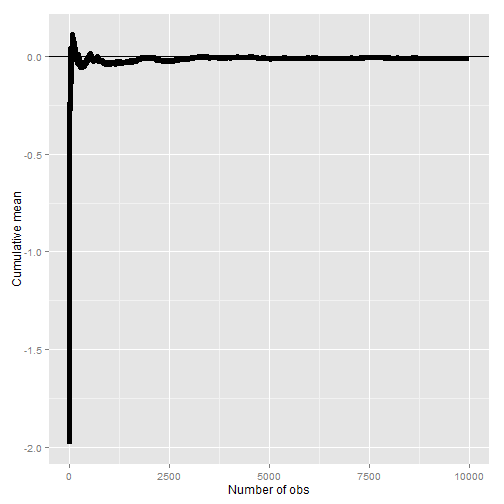
\includegraphics{LeanPub/images/normalLLN-1.png}
\caption{Cumulative average from standard normal simulations.}
\end{figure}

\subsubsection{Law of large numbers in action, coin
flip}\label{law-of-large-numbers-in-action-coin-flip}

Let's try the same thing, but for a fair coin flip. We'll simulate a lot
of coin flips and plot the cumulative proportion of heads.

\vspace{1pc}

\verb;Simulating many coinflips:;

\begin{Shaded}
\begin{Highlighting}[]
\NormalTok{means <-}\StringTok{ }\KeywordTok{cumsum}\NormalTok{(}\KeywordTok{sample}\NormalTok{(}\DecValTok{0}\NormalTok{:}\DecValTok{1}\NormalTok{, n, }\DataTypeTok{replace =} \OtherTok{TRUE}\NormalTok{))/(}\DecValTok{1}\NormalTok{:n)}
\NormalTok{g <-}\StringTok{ }\KeywordTok{ggplot}\NormalTok{(}\KeywordTok{data.frame}\NormalTok{(}\DataTypeTok{x =} \DecValTok{1}\NormalTok{:n, }\DataTypeTok{y =} \NormalTok{means), }\KeywordTok{aes}\NormalTok{(}\DataTypeTok{x =} \NormalTok{x, }\DataTypeTok{y =} \NormalTok{y))}
\NormalTok{g <-}\StringTok{ }\NormalTok{g +}\StringTok{ }\KeywordTok{geom_hline}\NormalTok{(}\DataTypeTok{yintercept =} \FloatTok{0.5}\NormalTok{) +}\StringTok{ }\KeywordTok{geom_line}\NormalTok{(}\DataTypeTok{size =} \DecValTok{2}\NormalTok{)}
\NormalTok{g <-}\StringTok{ }\NormalTok{g +}\StringTok{ }\KeywordTok{labs}\NormalTok{(}\DataTypeTok{x =} \StringTok{"Number of obs"}\NormalTok{, }\DataTypeTok{y =} \StringTok{"Cumulative mean"}\NormalTok{)}
\NormalTok{g}
\end{Highlighting}
\end{Shaded}

\begin{figure}[htbp]
\centering
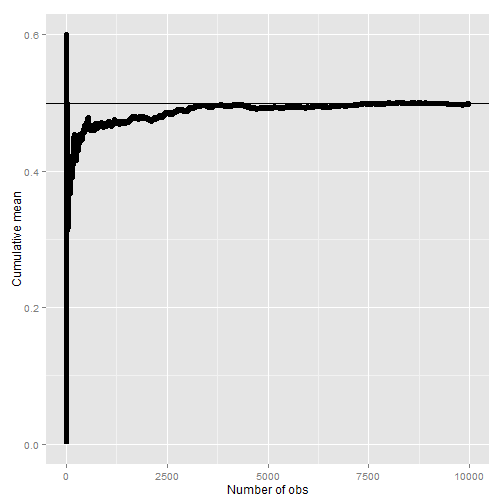
\includegraphics{LeanPub/images/coinLLN-1.png}
\caption{Cumulative proportion of heads from a sequence of coin flips.}
\end{figure}

\subsubsection{Discussion}\label{discussion}

An estimator is called \textbf{consistent} if it converges to what you
want to estimate. Thus, the LLN says that the sample mean of iid sample
is consistent for the population mean. Typically, good estimators are
consistent; it's not too much to ask that if we go to the trouble of
collecting an infinite amount of data that we get the right answer. The
sample variance and the sample standard deviation of iid random
variables are consistent as well.

\subsection{The Central Limit Theorem}\label{the-central-limit-theorem}

\href{http://youtu.be/FAIyVHmniK0?list=PLpl-gQkQivXiBmGyzLrUjzsblmQsLtkzJ}{Watch
this video before beginning.}

The \textbf{Central Limit Theorem} (CLT) is one of the most important
theorems in statistics. For our purposes, the CLT states that the
distribution of averages of iid variables becomes that of a standard
normal as the sample size increases. Consider this fact for a second. We
already know the mean and standard deviation of the distribution of
averages from iid samples. The CLT gives us an approximation to the full
distribution! Thus, for iid samples, we have a good sense of
distribution of the average event though: (1) we only observed one
average and (2) we don't know what the population distribution is.
Because of this, the CLT applies in an endless variety of settings and
is one of the most important theorems ever discovered.

The formal result is that

\[
\frac{\bar X_n - \mu}{\sigma / \sqrt{n}}=
\frac{\sqrt n (\bar X_n - \mu)}{\sigma}
= \frac{\mbox{Estimate} - \mbox{Mean of estimate}}{\mbox{Std. Err. of estimate}}
\]

has a distribution like that of a standard normal for large $n$.
Replacing the standard error by its estimated value doesn't change the
CLT.

The useful way to think about the CLT is that $\bar X_n$ is
approximately $N(\mu, \sigma^2 / n)$.

\subsection{CLT simulation
experiments}\label{clt-simulation-experiments}

Let's try simulating lots of averages from various distributions and
showing that the resulting distribution looks like a bell curve.

\subsubsection{Die rolling}\label{die-rolling}

\begin{itemize}
\itemsep1pt\parskip0pt\parsep0pt
\item
  Simulate a standard normal random variable by rolling $n$ (six sided)
  dice.
\item
  Let $X_i$ be the outcome for die $i$.
\item
  Then note that $\mu = E[X_i] = 3.5$.
\item
  Recall also that $Var(X_i) = 2.92$.
\item
  SE $\sqrt{2.92 / n} = 1.71 / \sqrt{n}$.
\item
  Lets roll $n$ dice, take their mean, subtract off 3.5, and divide by
  $1.71 / \sqrt{n}$ and repeat this over and over.
\end{itemize}

\begin{figure}[htbp]
\centering
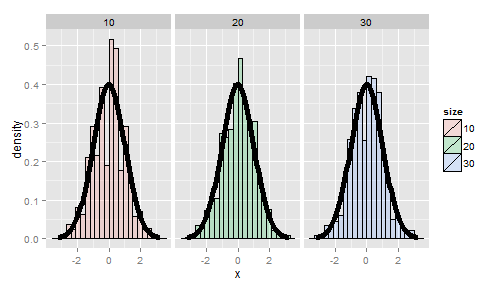
\includegraphics{LeanPub/images/dieCLT-1.png}
\caption{Result of die CLT simulation.}
\end{figure}

It's pretty remarkable that the approximation works so well with so few
rolls of the die. So, if you're stranded on an island, and need to
simulate a standard normal without a computer, but you do have a die,
you can get a pretty good approximation with 10 rolls even.

\subsubsection{Coin CLT}\label{coin-clt}

In fact the oldest application of the CLT is to the idea of flipping
coins
\href{http://en.wikipedia.org/wiki/De_Moivre\%E2\%80\%93Laplace_theorem}{(by
de Moivre)}. Let $X_i$ be the 0 or 1 result of the $i^{th}$ flip of a
possibly unfair coin. The sample proportion, say $\hat p$, is the
average of the coin flips. We know that:

\begin{itemize}
\itemsep1pt\parskip0pt\parsep0pt
\item
  $E[X_i] = p$,
\item
  $Var(X_i) = p(1-p)$,
\item
  $\sqrt{Var(\hat p)} = \sqrt{p(1-p)/n}$.
\end{itemize}

Furthermore, because of the CLT, we also know that:

\[
\frac{\hat p - p}{\sqrt{p(1-p)/n}}
\]

will be approximately normally distributed.

Let's test this by flipping a coin $n$ times, taking the sample
proportion of heads, subtract off 0.5 and multiply the result by
$2 \sqrt{n}$ (divide by $1/(2 \sqrt{n})$).

\begin{figure}[htbp]
\centering
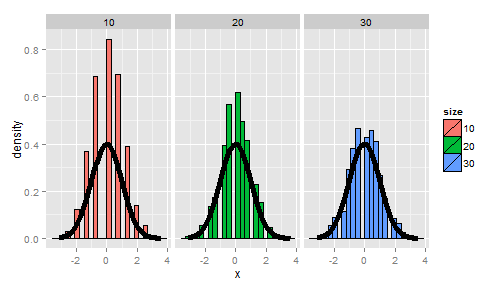
\includegraphics{LeanPub/images/coinCLT-1.png}
\caption{Results of the coin CLT simulation.}
\end{figure}

This convergence doesn't look quite as good as the die, since the coin
has fewer possible outcomes. In fact, among coins of various degrees of
bias, the convergence to normality is governed by how far from 0.5 $p$
is. Let's redo the simulation, now using $p=0.9$ instead of $p=0.5$ like
we did before.

\begin{figure}[htbp]
\centering
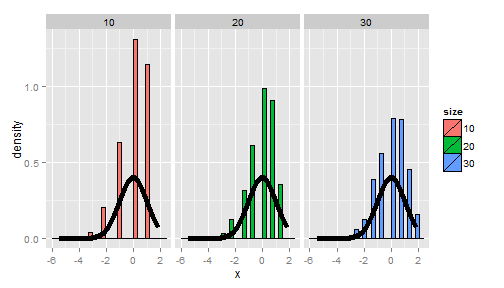
\includegraphics{LeanPub/images/coinCLT2-1.png}
\caption{Results of the simulation when p=0.9}
\end{figure}

Notice that the convergence to normality is quite poor. Thus, be careful
when using CLT approximations for sample proportions when your
proportion is very close to 0 or 1.

\subsection{Confidence intervals}\label{confidence-intervals}

\href{http://youtu.be/u85aQ0mtiZ8?list=PLpl-gQkQivXiBmGyzLrUjzsblmQsLtkzJ}{Watch
this video before beginning.}

Confidence intervals are methods for quantifying uncertainty in our
estimates. The fact that the interval has width characterizes that there
is randomness that prevents us from getting a perfect estimate. Let's go
through how a confidence interval using the CLT is constructed.

According to the CLT, the sample mean, $\bar X$, is approximately normal
with mean $\mu$ and standard deviation $\sigma / \sqrt{n}$. Furthermore,

\[\mu + 2 \sigma /\sqrt{n}\]

is pretty far out in the tail (only 2.5\% of a normal being larger than
2 sds in the tail). Similarly,

\[\mu - 2 \sigma /\sqrt{n}\]

is pretty far in the left tail (only 2.5\% chance of a normal being
smaller than 2 standard deviations in the tail). So the probability
$\bar X$ is bigger than $\mu + 2 \sigma / \sqrt{n}$ or smaller than
$\mu - 2 \sigma / \sqrt{n}$ is 5\%. Or equivalently, the probability
that these limits contain $\mu$ is 95\%. The quantity:

\[\bar X \pm 2 \sigma /\sqrt{n}\]

is called a 95\% interval for $\mu$. The 95\% refers to the fact that if
one were to repeatedly get samples of size $n$, about 95\% of the
intervals obtained would contain $\mu$. The 97.5th quantile is 1.96 (so
I rounded to 2 above). If instead of a 95\% interval, you wanted a 90\%
interval, then you want (100 - 90) / 2 = 5\% in each tail. Thus your
replace the 2 with the 95th percentile, which is 1.645.

\subsubsection{Example CI}\label{example-ci}

Give a confidence interval for the average height of sons in Galton's
data.

\vspace{1pc}

\verb;Finding a confidence interval.:;

\begin{Shaded}
\begin{Highlighting}[]
\KeywordTok{library}\NormalTok{(UsingR)}
\KeywordTok{data}\NormalTok{(father.son)}
\NormalTok{x <-}\StringTok{ }\NormalTok{father.son$sheight}
\NormalTok{(}\KeywordTok{mean}\NormalTok{(x) +}\StringTok{ }\KeywordTok{c}\NormalTok{(-}\DecValTok{1}\NormalTok{, }\DecValTok{1}\NormalTok{) *}\StringTok{ }\KeywordTok{qnorm}\NormalTok{(}\FloatTok{0.975}\NormalTok{) *}\StringTok{ }\KeywordTok{sd}\NormalTok{(x)/}\KeywordTok{sqrt}\NormalTok{(}\KeywordTok{length}\NormalTok{(x)))/}\DecValTok{12}
\end{Highlighting}
\end{Shaded}

\begin{verbatim}
## [1] 5.709670 5.737674
\end{verbatim}

Here we divided by 12 to get our interval in feet instead of inches. So
we estimate the average height of the sons as 5.71 to 5.74 with 95\%
confidence.

\subsubsection{Example using sample
proportions}\label{example-using-sample-proportions}

In the event that each $X_i$ is 0 or 1 with common success probability
$p$ then $\sigma^2 = p(1 - p)$. The interval takes the form:

\[
\hat p \pm z_{1 - \alpha/2}  \sqrt{\frac{p(1 - p)}{n}}.
\]

Replacing $p$ by $\hat p$ in the standard error results in what is
called a Wald confidence interval for $p$. Remember also that $p(1 - p)$
is maximized at 1/4. Plugging this in and setting our $Z$ quantile as 2
(which is about a 95\% interval) we find that a quick and dirty
confidence interval is:

\[\hat p \pm \frac{1}{\sqrt{n}}.\]

This is useful for doing quick confidence intervals for binomial
proportions in your head.

\subsubsection{Example}\label{example-15}

Your campaign advisor told you that in a random sample of 100 likely
voters, 56 intent to vote for you. Can you relax? Do you have this race
in the bag? Without access to a computer or calculator, how precise is
this estimate?

\begin{Shaded}
\begin{Highlighting}[]
\DecValTok{1}\NormalTok{/}\KeywordTok{sqrt}\NormalTok{(}\DecValTok{100}\NormalTok{)}
\end{Highlighting}
\end{Shaded}

\begin{verbatim}
## [1] 0.1
\end{verbatim}

so a back of the envelope calculation gives an approximate 95\% interval
of \texttt{(0.46, 0.66)}.

Thus, since the interval contains 0.5 and numbers below it, there's not
enough votes for you to relax; better go do more campaigning!

The basic rule of thumb is then, $1/\sqrt{n}$ gives you a good estimate
for the margin of error of a proportion. Thus, $n=100$\\for about 1
decimal place, 10,000 for 2, 1,000,000 for 3.

\begin{Shaded}
\begin{Highlighting}[]
\KeywordTok{round}\NormalTok{(}\DecValTok{1}\NormalTok{/}\KeywordTok{sqrt}\NormalTok{(}\DecValTok{10}\NormalTok{^(}\DecValTok{1}\NormalTok{:}\DecValTok{6}\NormalTok{)), }\DecValTok{3}\NormalTok{)}
\end{Highlighting}
\end{Shaded}

\begin{verbatim}
## [1] 0.316 0.100 0.032 0.010 0.003 0.001
\end{verbatim}

We could very easily do the full Wald interval, which is less
conservative (may provide a narrower interval). Remember the Wald
interval for a binomial proportion is:

\[
\hat p \pm Z_{1-\alpha/2} \sqrt{\frac{\hat p (1 - \hat p)}{n}}.
\]

Here's the R code for our election setting, both coding it directly and
using \texttt{binom.test}.

\begin{Shaded}
\begin{Highlighting}[]
\FloatTok{0.56} \NormalTok{+}\StringTok{ }\KeywordTok{c}\NormalTok{(-}\DecValTok{1}\NormalTok{, }\DecValTok{1}\NormalTok{) *}\StringTok{ }\KeywordTok{qnorm}\NormalTok{(}\FloatTok{0.975}\NormalTok{) *}\StringTok{ }\KeywordTok{sqrt}\NormalTok{(}\FloatTok{0.56} \NormalTok{*}\StringTok{ }\FloatTok{0.44}\NormalTok{/}\DecValTok{100}\NormalTok{)}
\end{Highlighting}
\end{Shaded}

\begin{verbatim}
## [1] 0.4627099 0.6572901
\end{verbatim}

\begin{Shaded}
\begin{Highlighting}[]
\KeywordTok{binom.test}\NormalTok{(}\DecValTok{56}\NormalTok{, }\DecValTok{100}\NormalTok{)$conf.int}
\end{Highlighting}
\end{Shaded}

\begin{verbatim}
## [1] 0.4571875 0.6591640
## attr(,"conf.level")
## [1] 0.95
\end{verbatim}

\subsection{Simulation of confidence
intervals}\label{simulation-of-confidence-intervals}

It is interesting to note that the coverage of confidence intervals
describes an aggregate behavior. In other words the confidence interval
describes the percentage of intervals that would cover the parameter
being estimated if we were to repeat the experiment over and over. So,
one can not technically say that the interval contains the parameter
with probability 95\%, say. So called Bayesian credible intervals
address this issue at the expense (or benefit depending on who you ask)
of adopting a Bayesian framework.

For our purposes, we're using confidence intervals and so will
investigate their frequency performance over repeated realizations of
the experiment. We can do this via simulation. Let's consider different
values of $p$ and look at the Wald interval's coverage when we
repeatedly create confidence intervals.

\vspace{1pc}

\verb;Code for investigating Wald interval coverage:;

\begin{Shaded}
\begin{Highlighting}[]
\NormalTok{n <-}\StringTok{ }\DecValTok{20}
\NormalTok{pvals <-}\StringTok{ }\KeywordTok{seq}\NormalTok{(}\FloatTok{0.1}\NormalTok{, }\FloatTok{0.9}\NormalTok{, }\DataTypeTok{by =} \FloatTok{0.05}\NormalTok{)}
\NormalTok{nosim <-}\StringTok{ }\DecValTok{1000}
\NormalTok{coverage <-}\StringTok{ }\KeywordTok{sapply}\NormalTok{(pvals, function(p) \{}
    \NormalTok{phats <-}\StringTok{ }\KeywordTok{rbinom}\NormalTok{(nosim, }\DataTypeTok{prob =} \NormalTok{p, }\DataTypeTok{size =} \NormalTok{n)/n}
    \NormalTok{ll <-}\StringTok{ }\NormalTok{phats -}\StringTok{ }\KeywordTok{qnorm}\NormalTok{(}\FloatTok{0.975}\NormalTok{) *}\StringTok{ }\KeywordTok{sqrt}\NormalTok{(phats *}\StringTok{ }\NormalTok{(}\DecValTok{1} \NormalTok{-}\StringTok{ }\NormalTok{phats)/n)}
    \NormalTok{ul <-}\StringTok{ }\NormalTok{phats +}\StringTok{ }\KeywordTok{qnorm}\NormalTok{(}\FloatTok{0.975}\NormalTok{) *}\StringTok{ }\KeywordTok{sqrt}\NormalTok{(phats *}\StringTok{ }\NormalTok{(}\DecValTok{1} \NormalTok{-}\StringTok{ }\NormalTok{phats)/n)}
    \KeywordTok{mean}\NormalTok{(ll <}\StringTok{ }\NormalTok{p &}\StringTok{ }\NormalTok{ul >}\StringTok{ }\NormalTok{p)}
\NormalTok{\})}
\end{Highlighting}
\end{Shaded}

\begin{figure}[htbp]
\centering
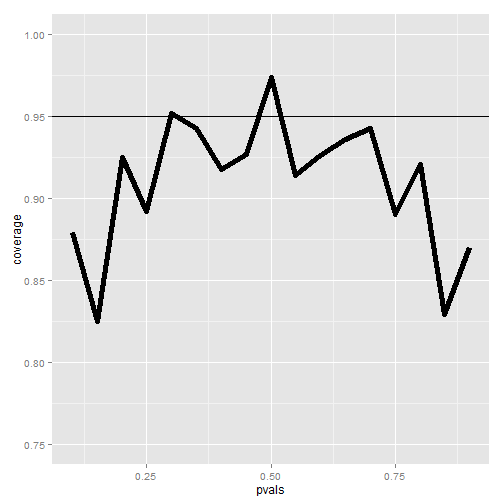
\includegraphics{LeanPub/images/waldCoverage-1.png}
\caption{Plot of Wald interval coverage.}
\end{figure}

The figure shows that if we were to repeatedly try experiments for any
fixed value of $p$, it's rarely the case that our intervals will cover
the value that they're trying to estimate in 95\% of them. This is bad,
since covering the parameter that its estimating 95\% of the time is the
confidence interval's only job!

So what's happening? Recall that the CLT is an approximation. In this
case $n$ isn't large enough for the CLT to be applicable for many of the
values of $p$. Let's see if the coverage improves for larger $n$.

\vspace{1pc}

\verb;Code for investigating Wald interval coverage:;

\begin{Shaded}
\begin{Highlighting}[]
\NormalTok{n <-}\StringTok{ }\DecValTok{100}
\NormalTok{pvals <-}\StringTok{ }\KeywordTok{seq}\NormalTok{(}\FloatTok{0.1}\NormalTok{, }\FloatTok{0.9}\NormalTok{, }\DataTypeTok{by =} \FloatTok{0.05}\NormalTok{)}
\NormalTok{nosim <-}\StringTok{ }\DecValTok{1000}
\NormalTok{coverage2 <-}\StringTok{ }\KeywordTok{sapply}\NormalTok{(pvals, function(p) \{}
    \NormalTok{phats <-}\StringTok{ }\KeywordTok{rbinom}\NormalTok{(nosim, }\DataTypeTok{prob =} \NormalTok{p, }\DataTypeTok{size =} \NormalTok{n)/n}
    \NormalTok{ll <-}\StringTok{ }\NormalTok{phats -}\StringTok{ }\KeywordTok{qnorm}\NormalTok{(}\FloatTok{0.975}\NormalTok{) *}\StringTok{ }\KeywordTok{sqrt}\NormalTok{(phats *}\StringTok{ }\NormalTok{(}\DecValTok{1} \NormalTok{-}\StringTok{ }\NormalTok{phats)/n)}
    \NormalTok{ul <-}\StringTok{ }\NormalTok{phats +}\StringTok{ }\KeywordTok{qnorm}\NormalTok{(}\FloatTok{0.975}\NormalTok{) *}\StringTok{ }\KeywordTok{sqrt}\NormalTok{(phats *}\StringTok{ }\NormalTok{(}\DecValTok{1} \NormalTok{-}\StringTok{ }\NormalTok{phats)/n)}
    \KeywordTok{mean}\NormalTok{(ll <}\StringTok{ }\NormalTok{p &}\StringTok{ }\NormalTok{ul >}\StringTok{ }\NormalTok{p)}
\NormalTok{\})}
\end{Highlighting}
\end{Shaded}

\begin{figure}[htbp]
\centering
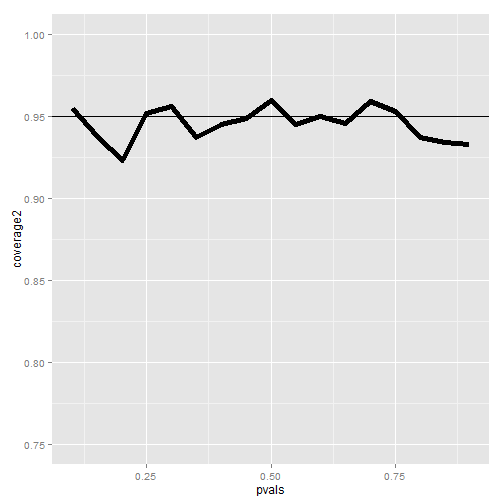
\includegraphics{LeanPub/images/waldCoverage2-1.png}
\caption{Output of simulation with $n=100$.}
\end{figure}

Now it looks much better. Of course, increasing our sample size is
rarely an option. There's exact fixes to make this interval work better
for small sample sizes.

However, for a quick fix is to take your data and add two successes and
two failures. So, for example, in our election example, we would form
our interval with 58 votes out of 104 sampled (disregarding that the
actual numbers were 56 and 100). This interval is called the
Agresti/Coull interval. This interval has much better coverage. Let's
show it via a simulation.

\vspace{1pc}

\verb;Code for investigating Agresti/Coull interval coverage when n=20.:;

\begin{Shaded}
\begin{Highlighting}[]
\NormalTok{n <-}\StringTok{ }\DecValTok{20}
\NormalTok{pvals <-}\StringTok{ }\KeywordTok{seq}\NormalTok{(}\FloatTok{0.1}\NormalTok{, }\FloatTok{0.9}\NormalTok{, }\DataTypeTok{by =} \FloatTok{0.05}\NormalTok{)}
\NormalTok{nosim <-}\StringTok{ }\DecValTok{1000}
\NormalTok{coverage <-}\StringTok{ }\KeywordTok{sapply}\NormalTok{(pvals, function(p) \{}
    \NormalTok{phats <-}\StringTok{ }\NormalTok{(}\KeywordTok{rbinom}\NormalTok{(nosim, }\DataTypeTok{prob =} \NormalTok{p, }\DataTypeTok{size =} \NormalTok{n) +}\StringTok{ }\DecValTok{2}\NormalTok{)/(n +}\StringTok{ }\DecValTok{4}\NormalTok{)}
    \NormalTok{ll <-}\StringTok{ }\NormalTok{phats -}\StringTok{ }\KeywordTok{qnorm}\NormalTok{(}\FloatTok{0.975}\NormalTok{) *}\StringTok{ }\KeywordTok{sqrt}\NormalTok{(phats *}\StringTok{ }\NormalTok{(}\DecValTok{1} \NormalTok{-}\StringTok{ }\NormalTok{phats)/n)}
    \NormalTok{ul <-}\StringTok{ }\NormalTok{phats +}\StringTok{ }\KeywordTok{qnorm}\NormalTok{(}\FloatTok{0.975}\NormalTok{) *}\StringTok{ }\KeywordTok{sqrt}\NormalTok{(phats *}\StringTok{ }\NormalTok{(}\DecValTok{1} \NormalTok{-}\StringTok{ }\NormalTok{phats)/n)}
    \KeywordTok{mean}\NormalTok{(ll <}\StringTok{ }\NormalTok{p &}\StringTok{ }\NormalTok{ul >}\StringTok{ }\NormalTok{p)}
\NormalTok{\})}
\end{Highlighting}
\end{Shaded}

\begin{figure}[htbp]
\centering
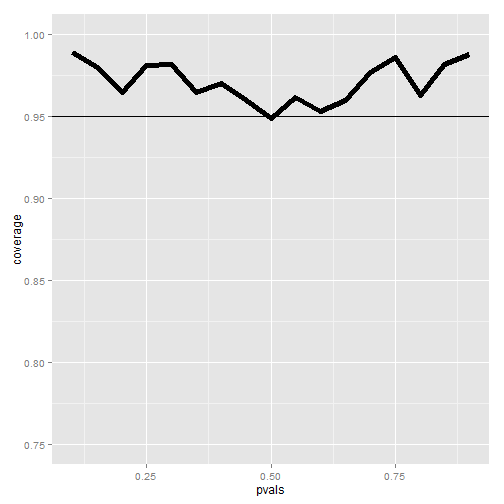
\includegraphics{LeanPub/images/agrestiCoull-1.png}
\caption{Coverage of the Agresti/Coull interval with $n=20$}
\end{figure}

The coverage is better, if maybe a little conservative in the sense of
being over the 95\% line most of the time. If the interval is too
conservative, it's likely a little too wide. To see this clearly,
imagine if we made our interval $-\infty$ to $\infty$. Then we would
always have 100\% coverage in any setting, but the interval wouldn't be
useful. Nonetheless, the Agrestic/Coull interval gives a much better
trade off between coverage and width than the Wald interval.

In general, one should use the add two successes and failures method for
binomial confidence intervals with smaller $n$. For very small $n$
consider using an exact interval (not covered in this class).

\subsection{Poisson interval}\label{poisson-interval}

Since the Poisson distribution is so central for data science, let's do
a Poisson confidence interval. Remember that if
$X \sim \mbox{Poisson}(\lambda t)$ then our estimate of $\lambda$ is
$\hat \lambda = X/t$. Furthermore, we know that
$Var(\hat \lambda) = \lambda / t$ and so the natural estimate is
$\hat \lambda / t$. While it's not immediate how the CLT applies in this
case, the interval is of the familiar form

\[
\mbox{Estimate} \pm Z_{1-\alpha/2} \mbox{SE}.
\]

So our Poisson interval is:

\[
\hat \lambda \pm  Z_{1-\alpha/2} \sqrt{\frac{\hat \lambda}{t}}
\]

\subsubsection{Example}\label{example-16}

A nuclear pump failed 5 times out of 94.32 days. Give a 95\% confidence
interval for the failure rate per day.

\vspace{1pc}

\verb;Code for asymptotic Poisson confidence interval:;

\begin{Shaded}
\begin{Highlighting}[]
\NormalTok{x <-}\StringTok{ }\DecValTok{5}
\NormalTok{t <-}\StringTok{ }\FloatTok{94.32}
\NormalTok{lambda <-}\StringTok{ }\NormalTok{x/t}
\KeywordTok{round}\NormalTok{(lambda +}\StringTok{ }\KeywordTok{c}\NormalTok{(-}\DecValTok{1}\NormalTok{, }\DecValTok{1}\NormalTok{) *}\StringTok{ }\KeywordTok{qnorm}\NormalTok{(}\FloatTok{0.975}\NormalTok{) *}\StringTok{ }\KeywordTok{sqrt}\NormalTok{(lambda/t), }\DecValTok{3}\NormalTok{)}
\end{Highlighting}
\end{Shaded}

\begin{verbatim}
## [1] 0.007 0.099
\end{verbatim}

A non-asymptotic test, one that guarantees coverage, is also available.
But, it has to be evaluated numerically.

\vspace{1pc}

\verb;Code for exact Poisson confidence interval:;

\begin{Shaded}
\begin{Highlighting}[]
\KeywordTok{poisson.test}\NormalTok{(x, }\DataTypeTok{T =} \FloatTok{94.32}\NormalTok{)$conf}
\end{Highlighting}
\end{Shaded}

\begin{verbatim}
## [1] 0.01721254 0.12371005
## attr(,"conf.level")
## [1] 0.95
\end{verbatim}

\subsubsection{Simulating the Poisson coverage
rate}\label{simulating-the-poisson-coverage-rate}

Let's see how the asymptotic interval performs for lambda values near
what we're estimating.

\vspace{1pc}

\verb;Code for evaluating the coverage of the asymptotic Poisson confidence interval:;

\begin{Shaded}
\begin{Highlighting}[]
\NormalTok{lambdavals <-}\StringTok{ }\KeywordTok{seq}\NormalTok{(}\FloatTok{0.005}\NormalTok{, }\FloatTok{0.1}\NormalTok{, }\DataTypeTok{by =} \FloatTok{0.01}\NormalTok{)}
\NormalTok{nosim <-}\StringTok{ }\DecValTok{1000}
\NormalTok{t <-}\StringTok{ }\DecValTok{100}
\NormalTok{coverage <-}\StringTok{ }\KeywordTok{sapply}\NormalTok{(lambdavals, function(lambda) \{}
    \NormalTok{lhats <-}\StringTok{ }\KeywordTok{rpois}\NormalTok{(nosim, }\DataTypeTok{lambda =} \NormalTok{lambda *}\StringTok{ }\NormalTok{t)/t}
    \NormalTok{ll <-}\StringTok{ }\NormalTok{lhats -}\StringTok{ }\KeywordTok{qnorm}\NormalTok{(}\FloatTok{0.975}\NormalTok{) *}\StringTok{ }\KeywordTok{sqrt}\NormalTok{(lhats/t)}
    \NormalTok{ul <-}\StringTok{ }\NormalTok{lhats +}\StringTok{ }\KeywordTok{qnorm}\NormalTok{(}\FloatTok{0.975}\NormalTok{) *}\StringTok{ }\KeywordTok{sqrt}\NormalTok{(lhats/t)}
    \KeywordTok{mean}\NormalTok{(ll <}\StringTok{ }\NormalTok{lambda &}\StringTok{ }\NormalTok{ul >}\StringTok{ }\NormalTok{lambda)}
\NormalTok{\})}
\end{Highlighting}
\end{Shaded}

\begin{figure}[htbp]
\centering
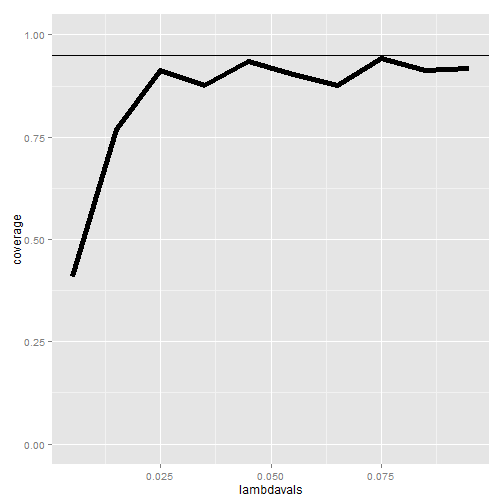
\includegraphics{LeanPub/images/poissonCoverage-1.png}
\caption{Coverage of Poisson intervals for various values of lambda}
\end{figure}

The coverage can be low for low values of lambda. In this case the
asymptotics works as we increase the monitoring time, t. Here's the
coverage if we increase $t$ to 1,000.

\begin{figure}[htbp]
\centering
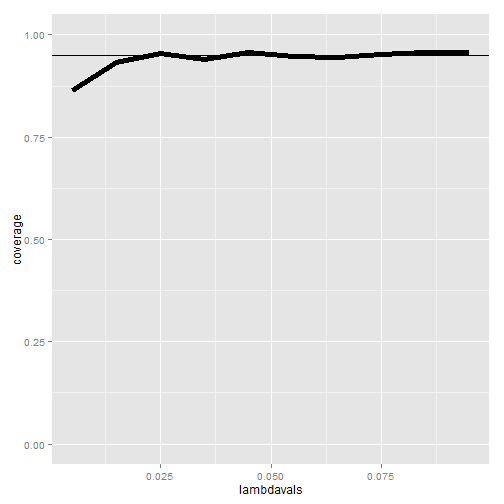
\includegraphics{LeanPub/images/poissonCoverage2-1.png}
\caption{Coverage of Poisson intervals for various values of lambda and
t=1000}
\end{figure}

\subsection{Summary notes}\label{summary-notes-4}

\begin{itemize}
\itemsep1pt\parskip0pt\parsep0pt
\item
  The LLN states that averages of iid samples. converge to the
  population means that they are estimating.
\item
  The CLT states that averages are approximately normal, with
  distributions.
\item
  centered at the population mean.
\item
  with standard deviation equal to the standard error of the mean.
\item
  CLT gives no guarantee that $n$ is large enough.
\item
  Taking the mean and adding and subtracting the relevant. normal
  quantile times the SE yields a confidence interval for the mean.
\item
  Adding and subtracting 2 SEs works for 95\% intervals.
\item
  Confidence intervals get wider as the coverage increases.
\item
  Confidence intervals get narrower with less variability or larger
  sample sizes.
\item
  The Poisson and binomial case have exact intervals that don't require
  the CLT.
\item
  But a quick fix for small sample size binomial calculations is to add
  2 successes and failures.
\end{itemize}

\subsection{Exercises}\label{exercises-6}

\begin{enumerate}
\def\labelenumi{\arabic{enumi}.}
\itemsep1pt\parskip0pt\parsep0pt
\item
  I simulate 1,000,000 standard normals. The LLN says that their sample
  average must be close to?
\item
  About what is the probability of getting 45 or fewer heads out 100
  flips of a fair coin? (Use the CLT, not the exact binomial
  calculation).
\item
  Consider the father.son data. Using the CLT and assuming that the
  fathers are a random sample from a population of interest, what is a
  95\% confidence mean height in inches?
\item
  The goal of a a confidence interval having coverage 95\% is to imply
  that:
\end{enumerate}

\begin{itemize}
\itemsep1pt\parskip0pt\parsep0pt
\item
  If one were to repeated collect samples and reconstruct the intervals,
  around 95\% percent of them would contain the true mean being
  estimated.
\item
  The probability that the sample mean is in the interval is 95\%.
\end{itemize}

\begin{enumerate}
\def\labelenumi{\arabic{enumi}.}
\setcounter{enumi}{4}
\itemsep1pt\parskip0pt\parsep0pt
\item
  The rate of search entries into a web site was 10 per minute when
  monitoring for an hour. Use R to calculate the exact Poisson interval
  for the rate of events per minute?
\item
  Consider a uniform distribution. If we were to sample 100 draws from a
  a uniform distribution (which has mean 0.5, and variance 1/12) and
  take their mean, $\bar X$. What is the approximate probability of
  getting as large as 0.51 or larger?
  \href{https://www.youtube.com/watch?v=JsiLK0g3IZ4\&index=15\&list=PLpl-gQkQivXhHOcVeU3bSJg78zaDYbP9L}{Watch
  this video solution} and
  \href{http://bcaffo.github.io/courses/06_StatisticalInference/homework/hw2.html\#9}{see
  the problem and solution here.}.
\end{enumerate}

\newpage

\section{\emph{t} Confidence intervals}\label{t-confidence-intervals}

\subsection{Small sample confidence
intervals}\label{small-sample-confidence-intervals}

\href{http://youtu.be/pHXrDMjzyYg?list=PLpl-gQkQivXiBmGyzLrUjzsblmQsLtkzJ}{Watch
this video before beginning.}

In the previous lecture, we discussed creating a confidence interval
using the CLT. Our intervals took the form:

\[Est \pm Z \times SE_{Est}.\]

In this lecture, we discuss some methods for small samples, notably
Gosset's \emph{t} distribution and \emph{t} confidence intervals.

These intervals are of the form:

\[Est \pm t \times SE_{Est}.\]

So the only change is that we've replaced the Z quantile now with a
\emph{t} quantile. These are some of the handiest of intervals in all of
statistics. If you want a rule between whether to use a \emph{t}
interval or normal interval, just always use the \emph{t} interval.

\subsection{Gosset's \emph{t}
distribution}\label{gossets-t-distribution}

The \emph{t} distribution was invented by William Gosset (under the
pseudonym ``Student'') in 1908. Fisher provided further mathematical
details about the distribution later. This distribution has thicker
tails than the normal. It's indexed by a degrees of freedom and it gets
more like a standard normal as the degrees of freedom get larger. It
assumes that the underlying data are iid Gaussian with the result that

\[
\frac{\bar X - \mu}{S/\sqrt{n}}
\]

follows Gosset's \emph{t} distribution with $n-1$ degrees of freedom.
(If we replaced $s$ by $\sigma$ the statistic would be exactly standard
normal.) The interval is

\[\bar X \pm t_{n-1} S/\sqrt{n},\]

where $t_{n-1}$ is the relevant quantile from the \emph{t} distribution.

\subsubsection{Code for manipulate}\label{code-for-manipulate}

You can use rStudio's manipulate function to to compare the \emph{t} and
Z distributions.

\vspace{1pc}

\verb;Code for investigating *t* and Z densities.:;

\begin{Shaded}
\begin{Highlighting}[]
\NormalTok{k <-}\StringTok{ }\DecValTok{1000}
\NormalTok{xvals <-}\StringTok{ }\KeywordTok{seq}\NormalTok{(-}\DecValTok{5}\NormalTok{, }\DecValTok{5}\NormalTok{, }\DataTypeTok{length =} \NormalTok{k)}
\NormalTok{myplot <-}\StringTok{ }\NormalTok{function(df)\{}
  \NormalTok{d <-}\StringTok{ }\KeywordTok{data.frame}\NormalTok{(}\DataTypeTok{y =} \KeywordTok{c}\NormalTok{(}\KeywordTok{dnorm}\NormalTok{(xvals), }\KeywordTok{dt}\NormalTok{(xvals, df)),}
                  \DataTypeTok{x =} \NormalTok{xvals,}
                  \DataTypeTok{dist =} \KeywordTok{factor}\NormalTok{(}\KeywordTok{rep}\NormalTok{(}\KeywordTok{c}\NormalTok{(}\StringTok{"Normal"}\NormalTok{, }\StringTok{"T"}\NormalTok{), }\KeywordTok{c}\NormalTok{(k,k))))}
  \NormalTok{g <-}\StringTok{ }\KeywordTok{ggplot}\NormalTok{(d, }\KeywordTok{aes}\NormalTok{(}\DataTypeTok{x =} \NormalTok{x, }\DataTypeTok{y =} \NormalTok{y))}
  \NormalTok{g <-}\StringTok{ }\NormalTok{g +}\StringTok{ }\KeywordTok{geom_line}\NormalTok{(}\DataTypeTok{size =} \DecValTok{2}\NormalTok{, }\KeywordTok{aes}\NormalTok{(}\DataTypeTok{color =} \NormalTok{dist))}
  \NormalTok{g}
\NormalTok{\}}
\KeywordTok{manipulate}\NormalTok{(}\KeywordTok{myplot}\NormalTok{(mu), }\DataTypeTok{mu =} \KeywordTok{slider}\NormalTok{(}\DecValTok{1}\NormalTok{, }\DecValTok{20}\NormalTok{, }\DataTypeTok{step =} \DecValTok{1}\NormalTok{))  }
\end{Highlighting}
\end{Shaded}

The difference is perhaps easier to see in the tails. Therefore, the
following code plots the upper quantiles of the Z distribution by those
of the \emph{t} distribution.

\vspace{1pc}

\verb;Code for investigating the upper quantiles of the *t* and Z densities.:;

\begin{Shaded}
\begin{Highlighting}[]
\NormalTok{pvals <-}\StringTok{ }\KeywordTok{seq}\NormalTok{(.}\DecValTok{5}\NormalTok{, .}\DecValTok{99}\NormalTok{, }\DataTypeTok{by =} \NormalTok{.}\DecValTok{01}\NormalTok{)}
\NormalTok{myplot2 <-}\StringTok{ }\NormalTok{function(df)\{}
  \NormalTok{d <-}\StringTok{ }\KeywordTok{data.frame}\NormalTok{(}\DataTypeTok{n=} \KeywordTok{qnorm}\NormalTok{(pvals),}\DataTypeTok{t=}\KeywordTok{qt}\NormalTok{(pvals, df),}
                  \DataTypeTok{p =} \NormalTok{pvals)}
  \NormalTok{g <-}\StringTok{ }\KeywordTok{ggplot}\NormalTok{(d, }\KeywordTok{aes}\NormalTok{(}\DataTypeTok{x=} \NormalTok{n, }\DataTypeTok{y =} \NormalTok{t))}
  \NormalTok{g <-}\StringTok{ }\NormalTok{g +}\StringTok{ }\KeywordTok{geom_abline}\NormalTok{(}\DataTypeTok{size =} \DecValTok{2}\NormalTok{, }\DataTypeTok{col =} \StringTok{"lightblue"}\NormalTok{)}
  \NormalTok{g <-}\StringTok{ }\NormalTok{g +}\StringTok{ }\KeywordTok{geom_line}\NormalTok{(}\DataTypeTok{size =} \DecValTok{2}\NormalTok{, }\DataTypeTok{col =} \StringTok{"black"}\NormalTok{)}
  \NormalTok{g <-}\StringTok{ }\NormalTok{g +}\StringTok{ }\KeywordTok{geom_vline}\NormalTok{(}\DataTypeTok{xintercept =} \KeywordTok{qnorm}\NormalTok{(}\FloatTok{0.975}\NormalTok{))}
  \NormalTok{g <-}\StringTok{ }\NormalTok{g +}\StringTok{ }\KeywordTok{geom_hline}\NormalTok{(}\DataTypeTok{yintercept =} \KeywordTok{qt}\NormalTok{(}\FloatTok{0.975}\NormalTok{, df))}
  \NormalTok{g}
\NormalTok{\}}
\KeywordTok{manipulate}\NormalTok{(}\KeywordTok{myplot2}\NormalTok{(df), }\DataTypeTok{df =} \KeywordTok{slider}\NormalTok{(}\DecValTok{1}\NormalTok{, }\DecValTok{20}\NormalTok{, }\DataTypeTok{step =} \DecValTok{1}\NormalTok{))}
\end{Highlighting}
\end{Shaded}

\subsubsection{Summary notes}\label{summary-notes-5}

In this section, we give an overview of important facts about the
\emph{t} distribution.

\begin{itemize}
\itemsep1pt\parskip0pt\parsep0pt
\item
  The \emph{t} interval technically assumes that the data are iid
  normal, though it is robust to this assumption.
\item
  It works well whenever the distribution of the data is roughly
  symmetric and mound shaped.
\item
  Paired observations are often analyzed using the \emph{t} interval by
  taking differences.
\item
  For large degrees of freedom, \emph{t} quantiles become the same as
  standard normal quantiles; therefore this interval converges to the
  same interval as the CLT yielded.
\item
  For skewed distributions, the spirit of the \emph{t} interval
  assumptions are violated.
\item
  Also, for skewed distributions, it doesn't make a lot of sense to
  center the interval at the mean.
\item
  In this case, consider taking logs or using a different summary like
  the median.
\item
  For highly discrete data, like binary, other intervals are available.
\end{itemize}

\subsubsection{Example of the \emph{t} interval, Gosset's sleep
data}\label{example-of-the-t-interval-gossets-sleep-data}

\href{http://youtu.be/2L41xqPvPso?list=PLpl-gQkQivXiBmGyzLrUjzsblmQsLtkzJ}{Watch
this video before beginning.}

In R typing brings up the sleep data originally analyzed in Gosset's
Biometrika paper, which shows the increase in hours for 10 patients on
two soporific drugs. R treats the data as two groups rather than paired.

\subsection{The data}\label{the-data}

\vspace{1pc}

\verb;Loading Galton's data.:;

\begin{Shaded}
\begin{Highlighting}[]
\KeywordTok{data}\NormalTok{(sleep)}
\KeywordTok{head}\NormalTok{(sleep)}
\end{Highlighting}
\end{Shaded}

\begin{verbatim}
##   extra group ID
## 1   0.7     1  1
## 2  -1.6     1  2
## 3  -0.2     1  3
## 4  -1.2     1  4
## 5  -0.1     1  5
## 6   3.4     1  6
\end{verbatim}

Here's a plot of the data. In this plot paired observations are
connected with a line.

\begin{figure}[htbp]
\centering
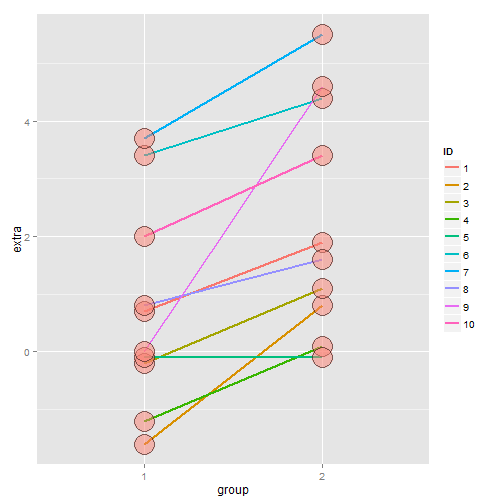
\includegraphics{LeanPub/images/galtonSleep-1.png}
\caption{A plot of the pairs of observations from Galton's sleep data.}
\end{figure}

Now let's calculate the \emph{t} interval for the differences from
baseline to follow up. Below we give four different ways for calculating
the interval.

\vspace{1pc}

\verb;*t* interval from baseline to follow up.:;

\begin{Shaded}
\begin{Highlighting}[]
\NormalTok{g1 <-}\StringTok{ }\NormalTok{sleep$extra[}\DecValTok{1} \NormalTok{:}\StringTok{ }\DecValTok{10}\NormalTok{]; g2 <-}\StringTok{ }\NormalTok{sleep$extra[}\DecValTok{11} \NormalTok{:}\StringTok{ }\DecValTok{20}\NormalTok{]}
\NormalTok{difference <-}\StringTok{ }\NormalTok{g2 -}\StringTok{ }\NormalTok{g1}
\NormalTok{mn <-}\StringTok{ }\KeywordTok{mean}\NormalTok{(difference); s <-}\StringTok{ }\KeywordTok{sd}\NormalTok{(difference); n <-}\StringTok{ }\DecValTok{10}
\NormalTok{## Calculating directly}
\NormalTok{mn +}\StringTok{ }\KeywordTok{c}\NormalTok{(-}\DecValTok{1}\NormalTok{, }\DecValTok{1}\NormalTok{) *}\StringTok{ }\KeywordTok{qt}\NormalTok{(.}\DecValTok{975}\NormalTok{, n}\DecValTok{-1}\NormalTok{) *}\StringTok{ }\NormalTok{s /}\StringTok{ }\KeywordTok{sqrt}\NormalTok{(n)}
\NormalTok{## using R's built in function}
\KeywordTok{t.test}\NormalTok{(difference)$conf.int[}\DecValTok{1}\NormalTok{:}\DecValTok{2}\NormalTok{]}
\NormalTok{## using R's built in function, another format}
\KeywordTok{t.test}\NormalTok{(g2, g1, }\DataTypeTok{paired =} \OtherTok{TRUE}\NormalTok{)$conf.int[}\DecValTok{1}\NormalTok{:}\DecValTok{2}\NormalTok{]}
\NormalTok{## using R's built in function, another format}
\KeywordTok{t.test}\NormalTok{(extra ~}\StringTok{ }\KeywordTok{I}\NormalTok{(}\KeywordTok{relevel}\NormalTok{(group, }\DecValTok{2}\NormalTok{)),}
       \DataTypeTok{paired =} \OtherTok{TRUE}\NormalTok{, }\DataTypeTok{data =} \NormalTok{sleep)$conf.int[}\DecValTok{1}\NormalTok{:}\DecValTok{2}\NormalTok{]}
\NormalTok{## Below are the results (after a little formatting)}
\end{Highlighting}
\end{Shaded}

\begin{verbatim}
## [1] 0.7001142 2.4598858
## [1] 0.7001142 2.4598858
## [1] 0.7001142 2.4598858
## [1] 0.7001142 2.4598858
\end{verbatim}

Therefore, since our interval doesn't include 0, our 95\% confidence
interval estimate for the mean change (follow up - baseline) is 0.70 to
2.45.

\subsection{Independent group \emph{t} confidence
intervals}\label{independent-group-t-confidence-intervals}

\href{http://youtu.be/J1XqN0yumEQ?list=PLpl-gQkQivXiBmGyzLrUjzsblmQsLtkzJ}{Watch
this video before beginning.}

Suppose that we want to compare the mean blood pressure between two
groups in a randomized trial; those who received the treatment to those
who received a placebo. The randomization is useful for attempting to
balance unobserved covariates that might contaminate our results.
Because of the randomization, it would be reasonable to compare the two
groups without considering further variables.

We cannot use the paired \emph{t} interval that we just used for
Galton's data, because the groups are independent. Person 1 from the
treated group has no relationship with person 1 from the control group.
Moreover, the groups may have different sample sizes, so taking paired
differences may not even be possible even if it isn't advisable in this
setting.

We now present methods for creating confidence intervals for comparing
independent groups.

\subsection{Confidence interval}\label{confidence-interval}

A $(1 - \alpha)\times 100\%$ confidence interval for the mean difference
between the groups, $\mu_y - \mu_x$ is:

\[
\bar Y - \bar X \pm t_{n_x + n_y - 2, 1 - \alpha/2}S_p
\left( \frac{1}{n_x} + \frac{1}{n_y} \right)^{1/2}.
\]

The notation $t_{n_x + n_y - 2, 1 - \alpha/2}$ means a \emph{t} quantile
with $n_x + n_y - 2$ degrees of freedom. The pooled variance estimator
is:

\[
S_p^2 = \{(n_x - 1) S_x^2 + (n_y - 1) S_y^2\}/(n_x + n_y - 2).
\]

This variance estimate is used if one is willing to assume a constant
variance across the groups. It is a weighted average of the
group-specific variances, with greater weight given to whichever group
has the larger sample size.

If there is some doubt about the constant variance assumption, assume a
different variance per group, which we will discuss later.

\subsection{Mistakenly treating the sleep data as
grouped}\label{mistakenly-treating-the-sleep-data-as-grouped}

Let's first go through an example where we treat paired data as if it
were independent. Consider Galton's sleep data from before. In the code
below, we do the R code for grouped data directly, and using the
\texttt{t.test} function.

\vspace{1pc}

\verb;Galton's data treated as grouped and independent.:;

\begin{Shaded}
\begin{Highlighting}[]
\NormalTok{n1 <-}\StringTok{ }\KeywordTok{length}\NormalTok{(g1); n2 <-}\StringTok{ }\KeywordTok{length}\NormalTok{(g2)}
\NormalTok{sp <-}\StringTok{ }\KeywordTok{sqrt}\NormalTok{( ((n1 -}\StringTok{ }\DecValTok{1}\NormalTok{) *}\StringTok{ }\KeywordTok{sd}\NormalTok{(g1)^}\DecValTok{2} \NormalTok{+}\StringTok{ }\NormalTok{(n2}\DecValTok{-1}\NormalTok{) *}\StringTok{ }\KeywordTok{sd}\NormalTok{(g2)^}\DecValTok{2}\NormalTok{) /}\StringTok{ }\NormalTok{(n1 +}\StringTok{ }\NormalTok{n2}\DecValTok{-2}\NormalTok{))}
\NormalTok{md <-}\StringTok{ }\KeywordTok{mean}\NormalTok{(g2) -}\StringTok{ }\KeywordTok{mean}\NormalTok{(g1)}
\NormalTok{semd <-}\StringTok{ }\NormalTok{sp *}\StringTok{ }\KeywordTok{sqrt}\NormalTok{(}\DecValTok{1} \NormalTok{/}\StringTok{ }\NormalTok{n1 +}\StringTok{ }\DecValTok{1}\NormalTok{/n2)}
\KeywordTok{rbind}\NormalTok{(}
  \NormalTok{md +}\StringTok{ }\KeywordTok{c}\NormalTok{(-}\DecValTok{1}\NormalTok{, }\DecValTok{1}\NormalTok{) *}\StringTok{ }\KeywordTok{qt}\NormalTok{(.}\DecValTok{975}\NormalTok{, n1 +}\StringTok{ }\NormalTok{n2 -}\StringTok{ }\DecValTok{2}\NormalTok{) *}\StringTok{ }\NormalTok{semd,  }
  \KeywordTok{t.test}\NormalTok{(g2, g1, }\DataTypeTok{paired =} \OtherTok{FALSE}\NormalTok{, }\DataTypeTok{var.equal =} \OtherTok{TRUE}\NormalTok{)$conf,}
  \KeywordTok{t.test}\NormalTok{(g2, g1, }\DataTypeTok{paired =} \OtherTok{TRUE}\NormalTok{)$conf}
\NormalTok{)}
\end{Highlighting}
\end{Shaded}

\begin{verbatim}
##            [,1]     [,2]
## [1,] -0.2038740 3.363874
## [2,] -0.2038740 3.363874
## [3,]  0.7001142 2.459886
\end{verbatim}

Notice that the paired interval (the last row) is entirely above zero.
The grouped interval (first two rows) contains zero. Thus, acknowledging
the pairing explains variation that would otherwise be absorbed into the
variation for the group means. As a result, treating the groups as
independent results in wider intervals. Even if it didn't result in a
shorter interval, the paired interval would be correct as the groups are
not statistically independent!

\subsubsection{\texttt{ChickWeight} data in
R}\label{chickweight-data-in-r}

Now let's try an example with actual independent groups. Load in the
\texttt{ChickWeight} data in R. We are also going to manipulate the
dataset to have a total weight gain variable using dplyr.

\begin{Shaded}
\begin{Highlighting}[]
\KeywordTok{library}\NormalTok{(datasets); }\KeywordTok{data}\NormalTok{(ChickWeight); }\KeywordTok{library}\NormalTok{(reshape2)}
\NormalTok{##define weight gain or loss}
\NormalTok{wideCW <-}\StringTok{ }\KeywordTok{dcast}\NormalTok{(ChickWeight, Diet +}\StringTok{ }\NormalTok{Chick ~}\StringTok{ }\NormalTok{Time,}
                \DataTypeTok{value.var =} \StringTok{"weight"}\NormalTok{)}
\KeywordTok{names}\NormalTok{(wideCW)[-(}\DecValTok{1} \NormalTok{:}\StringTok{ }\DecValTok{2}\NormalTok{)] <-}\StringTok{ }\KeywordTok{paste}\NormalTok{(}\StringTok{"time"}\NormalTok{,}
                                 \KeywordTok{names}\NormalTok{(wideCW)[-(}\DecValTok{1} \NormalTok{:}\StringTok{ }\DecValTok{2}\NormalTok{)],}
                                 \DataTypeTok{sep =} \StringTok{""}\NormalTok{)}
\KeywordTok{library}\NormalTok{(dplyr)}
\NormalTok{wideCW <-}\StringTok{ }\KeywordTok{mutate}\NormalTok{(wideCW,}
  \DataTypeTok{gain =} \NormalTok{time21 -}\StringTok{ }\NormalTok{time0}
\NormalTok{)}
\end{Highlighting}
\end{Shaded}

Here's a plot of the data.

\begin{figure}[htbp]
\centering
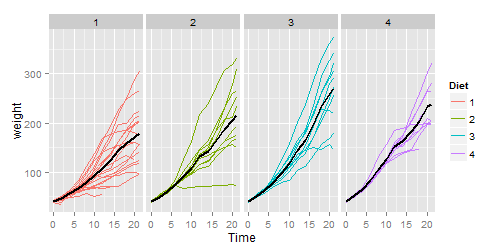
\includegraphics{LeanPub/images/chickweight-1.png}
\caption{Chickweight data over time.}
\end{figure}

Here's a plot only of the weight gain for the diets.

\begin{figure}[htbp]
\centering
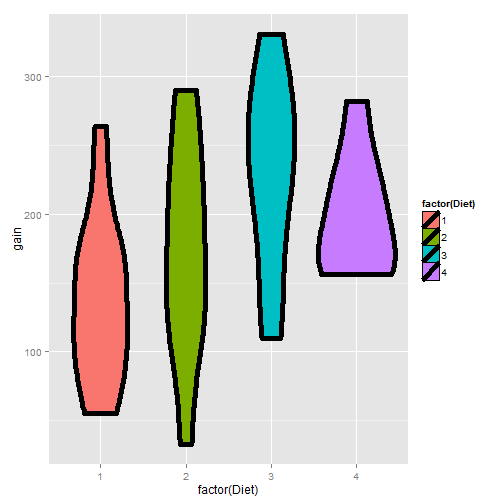
\includegraphics{LeanPub/images/chickweightgroups-1.png}
\caption{Violin plots of chickweight data by weight gain (final minus
baseline) by diet.}
\end{figure}

Now let's do a \emph{t} interval comparing groups 1 and 4. We'll show
the two intervals, one assuming that the variances are equal and one
assuming otherwise.

\vspace{1pc}

\verb;Code for t interval of the chickWeight data:;

\begin{Shaded}
\begin{Highlighting}[]
\NormalTok{wideCW14 <-}\StringTok{ }\KeywordTok{subset}\NormalTok{(wideCW, Diet %in%}\StringTok{ }\KeywordTok{c}\NormalTok{(}\DecValTok{1}\NormalTok{, }\DecValTok{4}\NormalTok{))}
\KeywordTok{rbind}\NormalTok{(}
  \KeywordTok{t.test}\NormalTok{(gain ~}\StringTok{ }\NormalTok{Diet, }\DataTypeTok{paired =} \OtherTok{FALSE}\NormalTok{, }\DataTypeTok{var.equal =} \OtherTok{TRUE}\NormalTok{,}
         \DataTypeTok{data =} \NormalTok{wideCW14)$conf,}
  \KeywordTok{t.test}\NormalTok{(gain ~}\StringTok{ }\NormalTok{Diet, }\DataTypeTok{paired =} \OtherTok{FALSE}\NormalTok{, }\DataTypeTok{var.equal =} \OtherTok{FALSE}\NormalTok{,}
         \DataTypeTok{data =} \NormalTok{wideCW14)$conf}
\NormalTok{)}
\end{Highlighting}
\end{Shaded}

\begin{verbatim}
##           [,1]      [,2]
## [1,] -108.1468 -14.81154
## [2,] -104.6590 -18.29932
\end{verbatim}

For the time being, let's interpret the equal variance interval. Since
the interval is entirely below zero it suggest that group 1 had less
weight gain than group 4 (at 95\% confidence).

\subsection{Unequal variances}\label{unequal-variances}

\href{https://www.youtube.com/watch?v=CVDdbR4VuOE\&list=PLpl-gQkQivXiBmGyzLrUjzsblmQsLtkzJ\&index=24}{Watch
this video before beginning.}

Under unequal variances our \emph{t} interval becomes:

\[
\bar Y - \bar X \pm t_{df} \times \left(\frac{s_x^2}{n_x} + \frac{s_y^2}{n_y}\right)^{1/2}
\]

where $t_{df}$ is the \emph{t} quantile calculated with degrees of
freedom:

\[
df=    \frac{\left(S_x^2 / n_x + S_y^2/n_y\right)^2}
    {\left(\frac{S_x^2}{n_x}\right)^2 / (n_x - 1) +
      \left(\frac{S_y^2}{n_y}\right)^2 / (n_y - 1)}
\]

which will be approximately a 95\% interval. This works really well. So
when in doubt, just assume unequal variances. Also, we present the
formula for completeness. In practice, it's easy to mess up, so make
sure to do \texttt{t.test}.

Referring back to the previous \texttt{ChickWeight} example, the violin
plots suggest that considering unequal variances would be wise. Recall
the code is

\begin{Shaded}
\begin{Highlighting}[]
\KeywordTok{t.test}\NormalTok{(gain ~}\StringTok{ }\NormalTok{Diet, }\DataTypeTok{paired =} \OtherTok{FALSE}\NormalTok{, }\DataTypeTok{var.equal =} \OtherTok{FALSE}\NormalTok{,}
       \DataTypeTok{data =} \NormalTok{wideCW14)$conf}
\end{Highlighting}
\end{Shaded}

\begin{verbatim}
## [1] -104.65901  -18.29932
## attr(,"conf.level")
## [1] 0.95
\end{verbatim}

This interval is remains entirely below zero. However, it is wider than
the equal variance interval.

\subsection{Summary notes}\label{summary-notes-6}

\begin{itemize}
\itemsep1pt\parskip0pt\parsep0pt
\item
  The \emph{t} distribution is useful for small sample size comparisons.
\item
  It technically assumes normality, but is robust to this assumption
  within limits.
\item
  The \emph{t} distribution gives rise to \emph{t} confidence intervals
  (and tests, which we will see later)
\end{itemize}

For other kinds of data, there are preferable small and large sample
intervals and tests.

\begin{itemize}
\itemsep1pt\parskip0pt\parsep0pt
\item
  For binomial data, there's lots of ways to compare two groups.
\item
  Relative risk, risk difference, odds ratio.
\item
  Chi-squared tests, normal approximations, exact tests.
\item
  For count data, there's also Chi-squared tests and exact tests.
\item
  We'll leave the discussions for comparing groups of data for binary
  and count data until covering glms in the regression class.
\item
  In addition, Mathematical Biostatistics Boot Camp 2 covers many
  special cases relevant to biostatistics.
\end{itemize}

\subsection{Exercises}\label{exercises-7}

\begin{enumerate}
\def\labelenumi{\arabic{enumi}.}
\itemsep1pt\parskip0pt\parsep0pt
\item
  For iid Gaussian data, the statistic
  $\frac{\bar X - \mu}{s / \sqrt{n}}$ must follow a:
\end{enumerate}

\begin{itemize}
\itemsep1pt\parskip0pt\parsep0pt
\item
  Z distribution
\item
  \emph{t} distribution
\end{itemize}

\begin{enumerate}
\def\labelenumi{\arabic{enumi}.}
\setcounter{enumi}{1}
\itemsep1pt\parskip0pt\parsep0pt
\item
  Paired differences T confidence intervals are useful when:
\end{enumerate}

\begin{itemize}
\itemsep1pt\parskip0pt\parsep0pt
\item
  Pairs of observations are linked, such as when there is subject level
  matching or in a study with baseline and follow up measurements on all
  participants.
\item
  When there was randomization of a treatment between two independent
  groups.
\end{itemize}

\begin{enumerate}
\def\labelenumi{\arabic{enumi}.}
\setcounter{enumi}{2}
\itemsep1pt\parskip0pt\parsep0pt
\item
  The assumption that the variances are equal for the independent group
  T interval means that:
\end{enumerate}

\begin{itemize}
\itemsep1pt\parskip0pt\parsep0pt
\item
  The sample variances have to be nearly identical.
\item
  The population variances are identical, but the sample variances may
  be different.
\end{itemize}

\begin{enumerate}
\def\labelenumi{\arabic{enumi}.}
\setcounter{enumi}{3}
\itemsep1pt\parskip0pt\parsep0pt
\item
  Load the data set \texttt{mtcars} in the \texttt{datasets} R package.
  Calculate a 95\% confidence interval to the nearest MPG for the
  variable \texttt{mpg}.
  \href{https://www.youtube.com/watch?v=5BPY6JqRLbE\&index=19\&list=PLpl-gQkQivXhHOcVeU3bSJg78zaDYbP9L}{Watch
  a video solution} and
  \href{http://bcaffo.github.io/courses/06_StatisticalInference/homework/hw3.html\#3}{see
  written solutions}.
\item
  Suppose that standard deviation of 9 paired differences is $1$. What
  value would the average difference have to be so that the lower
  endpoint of a 95\% students t confidence interval touches zero?
  \href{https://www.youtube.com/watch?v=ioDwUPCy508\&list=PLpl-gQkQivXhHOcVeU3bSJg78zaDYbP9L\&index=20}{Watch
  a video solution here} and
  \href{http://bcaffo.github.io/courses/06_StatisticalInference/homework/hw3.html\#4}{see
  the text here}.
\item
  An independent group Student's T interval is used instead of a paired
  T interval when:
\end{enumerate}

\begin{itemize}
\itemsep1pt\parskip0pt\parsep0pt
\item
  The observations are paired between the groups.
\item
  The observations between the groups are naturally assumed to be
  statistically independent.
\item
  As long as you do it correctly, either is fine.
\item
  More details are needed to answer this question.
  \href{https://www.youtube.com/watch?v=zJWJljxJ7Zk\&list=PLpl-gQkQivXhHOcVeU3bSJg78zaDYbP9L\&index=21}{watch
  a discussion of this problem} and
  \href{http://bcaffo.github.io/courses/06_StatisticalInference/homework/hw3.html\#5}{see
  the text.}
\end{itemize}

\begin{enumerate}
\def\labelenumi{\arabic{enumi}.}
\setcounter{enumi}{6}
\itemsep1pt\parskip0pt\parsep0pt
\item
  Consider the \texttt{mtcars} dataset. Construct a 95\% T interval for
  MPG comparing 4 to 6 cylinder cars (subtracting in the order of 4 - 6)
  assume a constant variance.
  \href{https://www.youtube.com/watch?v=QfuMgsUlu_w\&index=23\&list=PLpl-gQkQivXhHOcVeU3bSJg78zaDYbP9L}{Watch
  a video solution} and
  \href{http://bcaffo.github.io/courses/06_StatisticalInference/homework/hw3.html\#6}{see
  the text}. 10.
\item
  If someone put a gun to your head and said ``Your confidence interval
  must contain what it's estimating or I'll pull the trigger'', what
  would be the smart thing to do?
\end{enumerate}

\begin{itemize}
\itemsep1pt\parskip0pt\parsep0pt
\item
  Make your interval as wide as possible.
\item
  Make your interval as small as possible.
\item
  Call the authorities.
  \href{https://www.youtube.com/watch?v=8zM1RV4Rb7A\&list=PLpl-gQkQivXhHOcVeU3bSJg78zaDYbP9L\&index=24}{Watch
  the video solution} and
  \href{http://bcaffo.github.io/courses/06_StatisticalInference/homework/hw3.html\#7}{see
  the text.}
\end{itemize}

\begin{enumerate}
\def\labelenumi{\arabic{enumi}.}
\setcounter{enumi}{9}
\itemsep1pt\parskip0pt\parsep0pt
\item
  Refer back to comparing MPG for 4 versus 6 cylinders (question 7).
  What do you conclude?
\end{enumerate}

\begin{itemize}
\itemsep1pt\parskip0pt\parsep0pt
\item
  The interval is above zero, suggesting 6 is better than 4 in the terms
  of MPG.
\item
  The interval is above zero, suggesting 4 is better than 6 in the terms
  of MPG.
\item
  The interval does not tell you anything about the hypothesis test; you
  have to do the test.
\item
  The interval contains 0 suggesting no difference.
  \href{https://www.youtube.com/watch?v=zUVoueHLPdo\&index=25\&list=PLpl-gQkQivXhHOcVeU3bSJg78zaDYbP9L}{Watch
  a video solution} and
  \href{http://bcaffo.github.io/courses/06_StatisticalInference/homework/hw3.html\#8}{see
  the text.}
\end{itemize}

\begin{enumerate}
\def\labelenumi{\arabic{enumi}.}
\setcounter{enumi}{10}
\itemsep1pt\parskip0pt\parsep0pt
\item
  Suppose that 18 obese subjects were randomized, 9 each, to a new diet
  pill and a placebo. Subjects' body mass indices (BMIs) were measured
  at a baseline and again after having received the treatment or placebo
  for four weeks. The average difference from follow-up to the baseline
  (followup - baseline) was 3 kg/m2 for the treated group and 1 kg/m2
  for the placebo group. The corresponding standard deviations of the
  differences was 1.5 kg/m2 for the treatment group and 1.8 kg/m2 for
  the placebo group. The study aims to answer whether the change in BMI
  over the four week period appear to differ between the treated and
  placebo groups. What is the pooled variance estimate?
  \href{https://www.youtube.com/watch?v=kzRzrrDWTRQ\&index=26\&list=PLpl-gQkQivXhHOcVeU3bSJg78zaDYbP9L}{Watch
  a video solution here} and
  \href{http://bcaffo.github.io/courses/06_StatisticalInference/homework/hw3.html\#9}{see
  the text here.}
\end{enumerate}

\newpage

\section{Hypothesis testing}\label{hypothesis-testing}

Hypothesis testing is concerned with making decisions using data.

\subsection{Hypothesis testing}\label{hypothesis-testing-1}

\href{http://youtu.be/Wqvx6_12ZMs?list=PLpl-gQkQivXiBmGyzLrUjzsblmQsLtkzJ}{Watch
this video before beginning.}

To make decisions using data, we need to characterize the kinds of
conclusions we can make. Classical hypothesis testing is concerned with
deciding between two decisions (things get much harder if there's more
than two). The first, a null hypothesis is specified that represents the
status quo. This hypothesis is usually labeled, $H_0$. This is what we
assume by default. The alternative or research hypothesis is what we
require evidence to conclude. This hypothesis is usually labeled, $H_a$
or sometimes $H_1$ (or some other number other than 0).

So to reiterate, the null hypothesis is assumed true and statistical
evidence is required to reject it in favor of a research or alternative
hypothesis

\subsubsection{Example}\label{example-17}

A respiratory disturbance index (RDI) of more than 30 events / hour,
say, is considered evidence of severe sleep disordered breathing (SDB).
Suppose that in a sample of 100 overweight subjects with other risk
factors for sleep disordered breathing at a sleep clinic, the mean RDI
was 32 events / hour with a standard deviation of 10 events / hour.

We might want to test the hypothesis that

\[H_0 : \mu = 30\]

versus the hypothesis

\[H_a : \mu > 30\]

where $\mu$ is the population mean RDI. Clearly, somehow we must figure
out a way to decide between these hypotheses using the observed data,
particularly the sample mean.

Before we go through the specifics, let's set up the central ideas.

\subsection{Types of errors in hypothesis
testing}\label{types-of-errors-in-hypothesis-testing}

The alternative hypotheses are typically of the form of the true mean
being $<$, $>$ or $\neq$ to the hypothesized mean, such as
$H_a : \mu > 30$ from our example. The null typically sharply specifies
the mean, such as $H_0 : \mu = 30$ in our example. More complex null
hypotheses are possible, but are typically covered in later courses.

Note that there are four possible outcomes of our statistical decision
process:

\begin{longtable}[c]{@{}lll@{}}
\toprule\addlinespace
Truth & Decide & Result
\\\addlinespace
\midrule\endhead
$H_0$ & $H_0$ & Correctly accept null
\\\addlinespace
$H_0$ & $H_a$ & Type I error
\\\addlinespace
$H_a$ & $H_a$ & Correctly reject null
\\\addlinespace
$H_a$ & $H_0$ & Type II error
\\\addlinespace
\bottomrule
\end{longtable}

We will perform hypothesis testing by forcing the probability of a Type
I error to be small. This approach consequences, which we can discuss
with an analogy to court cases.

\subsection{Discussion relative to court
cases}\label{discussion-relative-to-court-cases}

Consider a court of law and a criminal case. The null hypothesis is that
the defendant is innocent. The rules requires a standard on the
available evidence to reject the null hypothesis (and the jury to
convict). The standard is specified loosely in this case, such as
convict if the defendant appears guilty ``Beyond reasonable doubt''. In
statistics, we can be mathematically specific about our standard of
evidence.

Note the consequences of setting a standard. If we set a low standard,
say convicting only if there circumstantial or greater evidence, then we
would increase the percentage of innocent people convicted (type I
errors). However, we would also increase the percentage of guilty people
convicted (correctly rejecting the null).

If we set a high standard, say the standard of convicting if the jury
has ``No doubts whatsoever'', then we increase the the percentage of
innocent people let free (correctly accepting the null) while we would
also increase the percentage of guilty people let free (type II errors).

\subsection{Building up a standard of
evidence}\label{building-up-a-standard-of-evidence}

\href{http://youtu.be/obNxIau2zrs?list=PLpl-gQkQivXiBmGyzLrUjzsblmQsLtkzJ}{Watch
this video before beginning.}

Consider our sleep example again. A reasonable strategy would reject the
null hypothesis if the sample mean, $\bar X$, was larger than some
constant, say $C$. Typically, $C$ is chosen so that the probability of a
Type I error, labeled $\alpha$, is $0.05$ (or some other relevant
constant) To reiterate, $\alpha =$ Type I error rate = Probability of
rejecting the null hypothesis when, in fact, the null hypothesis is
correct

Let's see if we can figure out what $C$ has to be. The standard error of
the mean is $10 / \sqrt{100} = 1$. Furthermore, under $H_0$ we know that
$\bar X \sim N(30, 1)$ (at least approximately) via the CLT. We want to
chose $C$ so that:

\[P(\bar X > C; H_0)=0.05.\]

The 95th percentile of a normal distribution is 1.645 standard
deviations from the mean. So, if $C$ is set 1.645 standard deviations
from the mean, we should be set since the probability of getting a
sample mean that large is only 5\%. The 95th percentile from a
$N(30, 1)$ is:

\[
C = 30 + 1 \times 1.645 = 31.645.
\]

So the rule ``Reject $H_0$ when $\bar X \geq 31.645$'' has the property
that the probability of rejection is 5\% when $H_0$ is true.

In general, however, we don't convert $C$ back to the original scale.
Instead, we calculate how many standard errors the observed mean is from
the hypothesized mean

\[
Z = \frac{\bar X - \mu_0}{s / \sqrt{n}}.
\]

This is called a Z-score. We can compare this statistic to standard
normal quantiles.

To reiterate, the Z-score is how many standard errors the sample mean is
above the hypothesized mean. In our example:

\[
\frac{32 - 30}{10 / \sqrt{100}} = 2
\]

Since 2 is greater than 1.645 we would reject. Setting the rule ``We
reject if our Z-score is larger than 1.645'' controls the Type I error
rate at 5\%. We could write out a general rule for this alternative
hypothesis as reject whenever
$\sqrt{n} (\bar X - \mu_0) / s > Z_{1-\alpha}$ where $\alpha$ is the
desired Type I error rate.

Because the Type I error rate was controlled to be small, if we reject
we know that one of the following occurred:

\begin{enumerate}
\def\labelenumi{\arabic{enumi}.}
\itemsep1pt\parskip0pt\parsep0pt
\item
  the null hypothesis is false,
\item
  we observed an unlikely event in support of the alternative even
  though the null is true,
\item
  our modeling assumptions are wrong.
\end{enumerate}

The third option can be difficult to check and at some level all bets
are off depending on how wrong we are about our basic assumptions. So
for this course, we speak of our conclusions under the assumption that
our modeling choices (such as the iid sampling model) are correct, but
do so wide eyed acknowledging the limitations of our approach.

\subsection{General rules}\label{general-rules}

We developed our test for one possible alternatives. Here's some general
rules for the three most important alternatives.

Consider the $Z$ test for $H_0:\mu = \mu_0$ versus: $H_1: \mu < \mu_0$,
$H_2: \mu \neq \mu_0$, $H_3: \mu > \mu_0$. Our test statistic

\[TS = \frac{\bar{X} - \mu_0}{S / \sqrt{n}}.\]

We reject the null hypothesis when:

\[H_1 : ~~~ TS \leq Z_{\alpha} = -Z_{1 - \alpha}\],

\[H_2 : ~~~ |TS| \geq Z_{1 - \alpha / 2}\]

\[H_3 : ~~~ TS \geq Z_{1 - \alpha}\],

respectively.

\subsubsection{Summary notes}\label{summary-notes-7}

\begin{itemize}
\itemsep1pt\parskip0pt\parsep0pt
\item
  We have fixed $\alpha$ to be low, so if we reject $H_0$ (either our
  model is wrong) or there is a low probability that we have made an
  error.
\item
  We have not fixed the probability of a type II error, $\beta$;
  therefore we tend to say ``Fail to reject $H_0$'' rather than
  accepting $H_0$.
\item
  Statistical significance is no the same as scientific significance.
\item
  The region of TS values for which you reject $H_0$ is called the
  rejection region.
\item
  The $Z$ test requires the assumptions of the CLT and for $n$ to be
  large enough for it to apply.
\item
  If $n$ is small, then a Gosset's \emph{t} test is performed exactly in
  the same way, with the normal quantiles replaced by the appropriate
  Student's \emph{t} quantiles and $n-1$ df.
\item
  The probability of rejecting the null hypothesis when it is false is
  called \textbf{power}
\item
  Power is a used a lot to calculate sample sizes for experiments.
\end{itemize}

\subsubsection{Example reconsidered}\label{example-reconsidered}

\href{http://youtu.be/5iMMBTlOFTI?list=PLpl-gQkQivXiBmGyzLrUjzsblmQsLtkzJ}{Watch
this video before beginning.}

Consider our example again. Suppose that $n= 16$ (rather than $100$).
The statistic

\[
\frac{\bar X - 30}{s / \sqrt{16}},
\]

follows a \emph{t} distribution with 15 df under $H_0$.

Under $H_0$, the probability that it is larger that the 95th percentile
of the \emph{t} distribution is 5\%. The 95th percentile of the T
distribution with 15 df is 1.7531 (obtained via 1.7530504).

Assuming that everything but the sample size is the same, our test
statistic is now $\sqrt{16}(32 - 30) / 10 = 0.8$. Since 0.8 is not
larger than 1.75, we now fail to reject.

\subsection{Two sided tests}\label{two-sided-tests}

In many settings, we would like to reject if the true mean is
\emph{different} than the hypothesized, not just larger or smaller. I
other words, we would reject the null hypothesis if in fact the sample
mean was much larger or smaller than the hypothesized mean. In our
example, we want to test the alternative $H_a : \mu \neq 30$.

We will reject if the test statistic, $0.8$, is either too large or too
small. Then we want the probability of rejecting under the null to be
5\%, split equally as 2.5\% in the upper tail and 2.5\% in the lower
tail.

Thus we reject if our test statistic is larger than
\texttt{qt(.975, 15)} or smaller than \texttt{qt(.025, 15)}. This is the
same as saying: reject if the absolute value of our statistic is larger
than \texttt{qt(0.975, 15)} = 2.1314.

In this case, since our test statistic is 0.8, which is smaller than
2.1314, we fail to reject the two sided test (as well as the one sided
test).

If you fail to reject the one sided test, then you would fail to reject
the two sided test. Because of its larger rejection region, two sided
tests are the norm (even in settings where a one sided test makes more
sense).

\subsection{T test in R}\label{t-test-in-r}

Let's try the \emph{t} test on the pairs of fathers and sons in Galton's
data.

\vspace{1pc}

\verb;Example of using the *t* test in R.:;

\begin{Shaded}
\begin{Highlighting}[]
\KeywordTok{library}\NormalTok{(UsingR); }\KeywordTok{data}\NormalTok{(father.son)}
\KeywordTok{t.test}\NormalTok{(father.son$sheight -}\StringTok{ }\NormalTok{father.son$fheight)}
\end{Highlighting}
\end{Shaded}

\begin{verbatim}
## 
##  One Sample t-test
## 
## data:  father.son$sheight - father.son$fheight
## t = 11.7885, df = 1077, p-value < 2.2e-16
## alternative hypothesis: true mean is not equal to 0
## 95 percent confidence interval:
##  0.8310296 1.1629160
## sample estimates:
## mean of x 
## 0.9969728
\end{verbatim}

\subsection{Connections with confidence
intervals}\label{connections-with-confidence-intervals}

Consider testing $H_0: \mu = \mu_0$ versus $H_a: \mu \neq \mu_0$. Take
the set of all possible values for which you fail to reject $H_0$, this
set is a $(1-\alpha)100\%$ confidence interval for $\mu$.

The same works in reverse; if a $(1-\alpha)100\%$ interval contains
$\mu_0$, then we \emph{fail to} reject $H_0$.

In other words, two sided tests and confidence intervals agree.

\subsection{Two group intervals}\label{two-group-intervals}

Doing group tests is now straightforward given that we've already
covered independent group T intervals. Our rejection rules are the same,
the only change is how the statistic is calculated. However, the form is
familiar:

\[
\frac{\mbox{Estimate} - \mbox{Hypothesized Value}}{\mbox{Standard Error}}.
\]

Consider now testing $H_0 : \mu_1 = \mu_2$. Our statistic is

\[
\frac{\bar X_1 - \bar X_2 - (\mu_1 - \mu_0)}{S_p\sqrt{\frac{1}{n1} + \frac{1}{n_2}}}.
\]

For the equal variance case and and

\[
\frac{\bar X_1 - \bar X_2 - (\mu_1 - \mu_0)}{\sqrt{\frac{S_1^2}{n1} + \frac{S_2^2}{n_2}}}.
\]

Let's just go through an example.

\subsubsection{Example \texttt{chickWeight}
data}\label{example-chickweight-data}

Recall that we reformatted this data as follows

\vspace{1pc}

\verb;Reformatting the data.:;

\begin{Shaded}
\begin{Highlighting}[]
\KeywordTok{library}\NormalTok{(datasets); }\KeywordTok{data}\NormalTok{(ChickWeight); }\KeywordTok{library}\NormalTok{(reshape2)}
\NormalTok{##define weight gain or loss}
\NormalTok{wideCW <-}\StringTok{ }\KeywordTok{dcast}\NormalTok{(ChickWeight, Diet +}\StringTok{ }\NormalTok{Chick ~}\StringTok{ }\NormalTok{Time,}
                \DataTypeTok{value.var =} \StringTok{"weight"}\NormalTok{)}
\KeywordTok{names}\NormalTok{(wideCW)[-(}\DecValTok{1} \NormalTok{:}\StringTok{ }\DecValTok{2}\NormalTok{)] <-}\StringTok{ }\KeywordTok{paste}\NormalTok{(}\StringTok{"time"}\NormalTok{,}
                                 \KeywordTok{names}\NormalTok{(wideCW)[-(}\DecValTok{1} \NormalTok{:}\StringTok{ }\DecValTok{2}\NormalTok{)],}
                                 \DataTypeTok{sep =} \StringTok{""}\NormalTok{)}
\KeywordTok{library}\NormalTok{(dplyr)}
\NormalTok{wideCW <-}\StringTok{ }\KeywordTok{mutate}\NormalTok{(wideCW,}
  \DataTypeTok{gain =} \NormalTok{time21 -}\StringTok{ }\NormalTok{time0}
\NormalTok{)}
\end{Highlighting}
\end{Shaded}

\vspace{1pc}

\verb;Unequal variance T test comparing diets 1 and 4.:;

\begin{Shaded}
\begin{Highlighting}[]
\NormalTok{wideCW14 <-}\StringTok{ }\KeywordTok{subset}\NormalTok{(wideCW, Diet %in%}\StringTok{ }\KeywordTok{c}\NormalTok{(}\DecValTok{1}\NormalTok{, }\DecValTok{4}\NormalTok{))}
\KeywordTok{t.test}\NormalTok{(gain ~}\StringTok{ }\NormalTok{Diet, }\DataTypeTok{paired =} \OtherTok{FALSE}\NormalTok{,}
       \DataTypeTok{var.equal =} \OtherTok{TRUE}\NormalTok{, }\DataTypeTok{data =} \NormalTok{wideCW14)}
\end{Highlighting}
\end{Shaded}

\begin{verbatim}
## 
##  Two Sample t-test
## 
## data:  gain by Diet
## t = -2.7252, df = 23, p-value = 0.01207
## alternative hypothesis: true difference in means is not equal to 0
## 95 percent confidence interval:
##  -108.14679  -14.81154
## sample estimates:
## mean in group 1 mean in group 4 
##        136.1875        197.6667
\end{verbatim}

\subsection{Exact binomial test}\label{exact-binomial-test}

Recall this problem. Suppose a friend has 8 children, 7 of which are
girls and none are twins.

Perform the relevant hypothesis test. $H_0 : p = 0.5$ versus
$H_a : p > 0.5$.

What is the relevant rejection region so that the probability of
rejecting is (less than) 5\%?

\begin{longtable}[c]{@{}ll@{}}
\toprule\addlinespace
Rejection region & Type I error rate
\\\addlinespace
\midrule\endhead
{[}0 : 8{]} & 1
\\\addlinespace
{[}1 : 8{]} & 0.9961
\\\addlinespace
{[}2 : 8{]} & 0.9648
\\\addlinespace
{[}3 : 8{]} & 0.8555
\\\addlinespace
{[}4 : 8{]} & 0.6367
\\\addlinespace
{[}5 : 8{]} & 0.3633
\\\addlinespace
{[}6 : 8{]} & 0.1445
\\\addlinespace
{[}7 : 8{]} & 0.0352
\\\addlinespace
{[}8 : 8{]} & 0.0039
\\\addlinespace
\bottomrule
\end{longtable}

Thus if we reject under 7 or 8 girls, we will have a less than 5\%
chance of rejecting under the null hypothesis.

It's impossible to get an exact 5\% level test for this case due to the
discreteness of the binomial. The closest is the rejection region {[}7 :
8{]}. Further note that an alpha level lower than 0.0039 is not
attainable. For larger sample sizes, we could do a normal approximation.

Extended this test to two sided test isn't obvious. Given a way to do
two sided tests, we could take the set of values of $p_0$ for which we
fail to reject to get an exact binomial confidence interval (called the
Clopper/Pearson interval, by the way). We'll cover two sided versions of
this test when we cover P-values.

\subsection{Exercises}\label{exercises-8}

\begin{enumerate}
\def\labelenumi{\arabic{enumi}.}
\itemsep1pt\parskip0pt\parsep0pt
\item
  Which hypothesis is typically assumed to be true in hypothesis
  testing?
\end{enumerate}

\begin{itemize}
\itemsep1pt\parskip0pt\parsep0pt
\item
  The null.
\item
  The alternative.
\end{itemize}

\begin{enumerate}
\def\labelenumi{\arabic{enumi}.}
\setcounter{enumi}{1}
\itemsep1pt\parskip0pt\parsep0pt
\item
  The type I error rate controls what?
\item
  Load the data set \texttt{mtcars} in the \texttt{datasets} R package.
  Assume that the data set mtcars is a random sample. Compute the mean
  MPG, $\bar x,$ of this sample. You want to test whether the true MPG
  is $\mu_0$ or smaller using a one sided 5\% level test.
  ($H_0 : \mu = \mu_0$ versus $H_a : \mu < \mu_0$). Using that data set
  and a Z test: Based on the mean MPG of the sample $\bar x,$ and by
  using a Z test: what is the smallest value of $\mu_0$ that you would
  reject for (to two decimal places)?
  \href{https://www.youtube.com/watch?v=gReR0uxLnIA\&list=PLpl-gQkQivXhHOcVeU3bSJg78zaDYbP9L\&index=27}{Watch
  a video solution here} and
  \href{http://bcaffo.github.io/courses/06_StatisticalInference/homework/hw4.html\#3}{see
  the text here}.
\item
  Consider again the \texttt{mtcars} dataset. Use a two group t-test to
  test the hypothesis that the 4 and 6 cyl cars have the same mpg. Use a
  two sided test with unequal variances. Do you reject?
  \href{https://www.youtube.com/watch?v=Zo5TirzS9rU\&list=PLpl-gQkQivXhHOcVeU3bSJg78zaDYbP9L\&index=28}{Watch
  the video here} and
  \href{http://bcaffo.github.io/courses/06_StatisticalInference/homework/hw4.html\#4}{see
  the text here}
\item
  A sample of 100 men yielded an average PSA level of 3.0 with a sd of
  1.1. What are the complete set of values that a 5\% two sided Z test
  of $H_0 : \mu = \mu_0$ would fail to reject the null hypothesis for?
  \href{https://www.youtube.com/watch?v=TooyEaVgLZc\&list=PLpl-gQkQivXhHOcVeU3bSJg78zaDYbP9L\&index=29}{Watch
  the video solution} and
  \href{http://bcaffo.github.io/courses/06_StatisticalInference/homework/hw4.html\#5}{see
  the text}.
\item
  You believe the coin that you're flipping is biased towards heads. You
  get 55 heads out of 100 flips. Do you reject at the 5\% level that the
  coin is fair?
  \href{https://www.youtube.com/watch?v=0sqOErsfhqo\&list=PLpl-gQkQivXhHOcVeU3bSJg78zaDYbP9L\&index=30}{Watch
  a video solution} and
  \href{http://bcaffo.github.io/courses/06_StatisticalInference/homework/hw4.html\#6}{see
  the text}.
\item
  Suppose that in an AB test, one advertising scheme led to an average
  of 10 purchases per day for a sample of 100 days, while the other led
  to 11 purchases per day, also for a sample of 100 days. Assuming a
  common standard deviation of 4 purchases per day. Assuming that the
  groups are independent and that they days are iid, perform a Z test of
  equivalence. Do you reject at the 5\% level?
  \href{https://www.youtube.com/watch?v=Or4ly4rOiaA\&index=32\&list=PLpl-gQkQivXhHOcVeU3bSJg78zaDYbP9L}{Watch
  a video solution} and
  \href{http://bcaffo.github.io/courses/06_StatisticalInference/homework/hw4.html\#8}{see
  the text.}
\item
  A confidence interval for the mean contains:
\end{enumerate}

\begin{itemize}
\itemsep1pt\parskip0pt\parsep0pt
\item
  All of the values of the hypothesized mean for which we would fail to
  reject with $\alpha = 1 - Conf. Level$.
\item
  All of the values of the hypothesized mean for which we would fail to
  reject with $2 \alpha = 1 - Conf. Level$.
\item
  All of the values of the hypothesized mean for which we would reject
  with $\alpha = 1 - Conf. Level$.
\item
  All of the values of the hypothesized mean for which we would reject
  with $2 \alpha = 1 - Conf. Level$.
  \href{https://www.youtube.com/watch?v=UiNV1mXQGLs\&index=33\&list=PLpl-gQkQivXhHOcVeU3bSJg78zaDYbP9L}{Watch
  a video solution} and
  \href{http://bcaffo.github.io/courses/06_StatisticalInference/homework/hw4.html\#9}{see
  the text}.
\end{itemize}

\begin{enumerate}
\def\labelenumi{\arabic{enumi}.}
\setcounter{enumi}{8}
\itemsep1pt\parskip0pt\parsep0pt
\item
  In a court of law, all things being equal, if via policy you require a
  lower standard of evidence to convict people then
\end{enumerate}

\begin{itemize}
\itemsep1pt\parskip0pt\parsep0pt
\item
  Less guilty people will be convicted.
\item
  More innocent people will be convicted.
\item
  More Innocent people will be not convicted.
  \href{https://www.youtube.com/watch?v=GlKPG24bZMI\&index=36\&list=PLpl-gQkQivXhHOcVeU3bSJg78zaDYbP9L}{Watch
  a video solution} and
  \href{http://bcaffo.github.io/courses/06_StatisticalInference/homework/hw4.html\#12}{see
  the text}.
\end{itemize}

\newpage

\section{P-values}\label{p-values}

\subsection{Introduction to P-values}\label{introduction-to-p-values}

\href{http://youtu.be/Ky68x_7iK6c?list=PLpl-gQkQivXiBmGyzLrUjzsblmQsLtkzJ}{Watch
this video before beginning.}

P-values are the most common measure of statistical significance. Their
ubiquity, along with concern over their interpretation and use makes
them controversial among statisticians. The following manuscripts are
interesting reads about P-values.

\begin{itemize}
\itemsep1pt\parskip0pt\parsep0pt
\item
  \url{http://warnercnr.colostate.edu/~anderson/thompson1.html}
\item
  \href{http://www.crcpress.com/product/isbn/9780412044113}{Also see
  \emph{Statistical Evidence: A Likelihood Paradigm} by Richard Royall}
\item
  \href{https://scholar.google.com/scholar?q=towards+evidence+based+medical+statistics+the+p-value+fallacy\&hl=en\&as_sdt=0\&as_vis=1\&oi=scholart\&sa=X\&ei=uOTjVNHdG4anggSMlYOwBQ\&ved=0CBsQgQMwAA}{\emph{Toward
  Evidence-Based Medical Statistics. 1: The P Value Fallacy} by Steve
  Goodman}
\item
  The hilariously titled:
  \href{http://www.scopus.com/record/display.url?eid=2-s2.0-0039802908\&origin=inward\&txGid=BBE363C58BE8785BFF9E71AB60004733.ZmAySxCHIBxxTXbnsoe5w\%3a2}{\emph{The
  Earth is Round (p \textless{} .05)} by Cohen.}
\item
  Some positive comments
\item
  \href{http://simplystatistics.org/2012/01/06/p-values-and-hypothesis-testing-get-a-bad-rap-but-we/}{simply
  statistics}
\item
  \href{http://normaldeviate.wordpress.com/2013/03/14/double-misunderstandings-about-p-values/}{normal
  deviate}
\item
  \href{http://errorstatistics.com/2013/06/14/p-values-cant-be-trusted-except-when-used-to-argue-that-p-values-cant-be-trusted/}{Error
  statistics}
\end{itemize}

\subsection{What is a P-value?}\label{what-is-a-p-value}

The central idea of a P-value is to assume that the null hypothesis is
true and calculate how unusual it would be to see data (in the form of a
test statistic) as extreme as was seen in favor of the alternative
hypothesis. The formal definition is:

A \textbf{P-value} is the probability of observing a test statistic as
or more extreme in favor of the alternative than was actually obtained,
where the probability is calculated assuming that the null hypothesis is
true.

A P-value then requires a few steps. 1. Decide on a statistic that
evaluates support of the null or alternative hypothesis. 2. Decide on a
distribution of that statistic under the null hypothesis (null
distribution). 3. Calculate the probability of obtaining a statistic as
or more extreme as was observed using the distribution in 2.

The way to interpret P-values is as follows. If the P-value is small,
then either $H_0$ is true and we have observed a rare event or $H_0$ is
false (or possibly the null model is incorrect).

Let's do a quick example. Suppose that you get a \emph{t} statistic of
2.5 for 15 degrees of freedom testing $H_0:\mu = \mu_0$ versus
$H_a : \mu > \mu_0$. What's the probability of getting a \emph{t}
statistic as large as 2.5?

\vspace{1pc}

\verb;P-value calculation in R.:;

\begin{Shaded}
\begin{Highlighting}[]
\KeywordTok{pt}\NormalTok{(}\FloatTok{2.5}\NormalTok{, }\DecValTok{15}\NormalTok{, }\DataTypeTok{lower.tail =} \OtherTok{FALSE}\NormalTok{)}
\end{Highlighting}
\end{Shaded}

\begin{verbatim}
## [1] 0.0122529
\end{verbatim}

Therefore, the probability of seeing evidence as extreme or more extreme
than that actually obtained under $H_0$ is 0.0123. So, (assuming our
model is correct) either we observed data that was pretty unlikely under
the null, or the null hypothesis if false.

\subsection{The attained significance
level}\label{the-attained-significance-level}

Recall in a previous chapter that our test statistic was 2 for
$H_0 : \mu_0  = 30$ versus $H_a:\mu > 30$ using a normal test ($n$ was
100). Notice that we rejected the one sided test when $\alpha = 0.05$,
would we reject if $\alpha = 0.01$, how about 0.001?

The smallest value for alpha that you still reject the null hypothesis
is called the \emph{attained significance level}. This is mathematically
equivalent, but philosophically a little different from, the
\emph{P-value}. Whereas the P-value is interpreted in the terms of how
probabilistically extreme our test statistic is under the null, the
attained significance level merely conveys what the smallest level of
$\alpha$ that one could reject at.

This equivalence makes P-values very convenient to convey. The reader of
the results can perform the test at whatever $\alpha$ he or she choses.
This is especially useful in multiple testing circumstances.

Here's the two rules for performing hypothesis tests with P-values. * If
the P-value for a test is less than $\alpha$ you reject the null
hypothesis * For two sided hypothesis test, double the smaller of the
two one sided hypothesis test Pvalues

\subsection{Binomial P-value example}\label{binomial-p-value-example}

Suppose a friend has 8 children, 7 of which are girls and none are
twins. If each gender has an independent 50\% probability for each
birth, what's the probability of getting 7 or more girls out of 8
births?

This calculation is a P-value where the statistic is the number of girls
and the null distribution is a fair coin flip for each gender. We want
to test $H_0: p=0.5$ versus $H_a: p > 0.5$, where $p$ is the probability
of having a girl for each birth.

Recall here's the calculation:

\vspace{1pc}

\verb;Example of a Binomial P-value calculation in R.:;

\begin{Shaded}
\begin{Highlighting}[]
\KeywordTok{pbinom}\NormalTok{(}\DecValTok{6}\NormalTok{, }\DataTypeTok{size =} \DecValTok{8}\NormalTok{, }\DataTypeTok{prob =} \FloatTok{0.5}\NormalTok{, }\DataTypeTok{lower.tail =} \OtherTok{FALSE}\NormalTok{)}
\end{Highlighting}
\end{Shaded}

\begin{verbatim}
## [1] 0.03515625
\end{verbatim}

Since our P-value is less than 0.05 we would reject at a 5\% error rate.
Note, however, if we were doing a two sided test, we would have to
double the P-value and thus would then fail to reject.

\subsection{Poisson example}\label{poisson-example}

\href{http://youtu.be/Tcw2OVyEX3s?list=PLpl-gQkQivXiBmGyzLrUjzsblmQsLtkzJ}{Watch
this video before beginning.}

Suppose that a hospital has an infection rate of 10 infections per 100
person/days at risk (rate of 0.1) during the last monitoring period.
Assume that an infection rate of 0.05 is an important benchmark.

Given a Poisson model, could the observed rate being larger than 0.05 be
attributed to chance? We want to test $H_0: \lambda = 0.05$ where
$\lambda$ is the rate of infections per person day so that 5 would be
the rate per 100 days. Thus we want to know if 9 events per 100
person/days is unusual with respect to a Poisson distribution with a
rate of 5 events per 100. Consider $H_a: \lambda > 0.05$.

\vspace{1pc}

\verb;Poisson P-value calculation.:;

\begin{Shaded}
\begin{Highlighting}[]
\KeywordTok{ppois}\NormalTok{(}\DecValTok{9}\NormalTok{, }\DecValTok{5}\NormalTok{, }\DataTypeTok{lower.tail =} \OtherTok{FALSE}\NormalTok{)}
\end{Highlighting}
\end{Shaded}

\begin{verbatim}
## [1] 0.03182806
\end{verbatim}

Again, since this P-value is less than 0.05 we reject the null
hypothesis. The P-value would be 0.06 for two sided hypothesis (double)
and so we would fail to reject in that case.

\subsection{Exercises}\label{exercises-9}

\begin{enumerate}
\def\labelenumi{\arabic{enumi}.}
\itemsep1pt\parskip0pt\parsep0pt
\item
  P-values are probabilities that are calculated assuming which
  hypothesis is true?
\end{enumerate}

\begin{itemize}
\itemsep1pt\parskip0pt\parsep0pt
\item
  the alternative
\item
  the null
\end{itemize}

\begin{enumerate}
\def\labelenumi{\arabic{enumi}.}
\setcounter{enumi}{1}
\itemsep1pt\parskip0pt\parsep0pt
\item
  You get a P-value of 0.06. Would you reject for a type I error rate of
  0.05?
\end{enumerate}

\begin{itemize}
\itemsep1pt\parskip0pt\parsep0pt
\item
  Yes you would reject the null
\item
  No you would not reject the null
\item
  It depends on information not given
\end{itemize}

\begin{enumerate}
\def\labelenumi{\arabic{enumi}.}
\setcounter{enumi}{2}
\itemsep1pt\parskip0pt\parsep0pt
\item
  The proposed procedure for getting a two sided P-value for the exact
  binomial test considered here is what?
\end{enumerate}

\begin{itemize}
\itemsep1pt\parskip0pt\parsep0pt
\item
  Multiplying the one sided P-value by one half
\item
  Doubling the larger of the two one sided P-values
\item
  Doubling the smaller of the two one sided P-values
\item
  No procedure exists
\end{itemize}

\begin{enumerate}
\def\labelenumi{\arabic{enumi}.}
\setcounter{enumi}{3}
\itemsep1pt\parskip0pt\parsep0pt
\item
  Consider again the \texttt{mtcars} dataset. Use a two group t-test to
  test the hypothesis that the 4 and 6 cyl cars have the same mpg. Use a
  two sided test with unequal variances. Give a P-value.
  \href{https://www.youtube.com/watch?v=Zo5TirzS9rU\&list=PLpl-gQkQivXhHOcVeU3bSJg78zaDYbP9L\&index=28}{Watch
  the video here} and
  \href{http://bcaffo.github.io/courses/06_StatisticalInference/homework/hw4.html\#4}{see
  the text here}
\item
  You believe the coin that you're flipping is biased towards heads. You
  get 55 heads out of 100 flips. Give an exact P-value for the
  hypothesis that the coin is fair.
  \href{https://www.youtube.com/watch?v=0sqOErsfhqo\&list=PLpl-gQkQivXhHOcVeU3bSJg78zaDYbP9L\&index=30}{Watch
  a video solution} and
  \href{http://bcaffo.github.io/courses/06_StatisticalInference/homework/hw4.html\#6}{see
  the text}.
\item
  A web site was monitored for a year and it received 520 hits per day.
  In the first 30 days in the next year, the site received 15,800 hits.
  Assuming that web hits are Poisson. Give an exact one sided P-value to
  the hypothesis that web hits are up this year over last. Do you
  reject?
  \href{https://www.youtube.com/watch?v=cE_88-Q7TX0\&index=31\&list=PLpl-gQkQivXhHOcVeU3bSJg78zaDYbP9L}{Watch
  the video solutions} and
  \href{http://bcaffo.github.io/courses/06_StatisticalInference/homework/hw4.html\#7}{see
  the problem text}.
\item
  Suppose that in an AB test, one advertising scheme led to an average
  of 10 purchases per day for a sample of 100 days, while the other led
  to 11 purchases per day, also for a sample of 100 days. Assuming a
  common standard deviation of 4 purchases per day. Assuming that the
  groups are independent and that they days are iid, perform a Z test of
  equivalence. Give a P-value for the test?
  \href{https://www.youtube.com/watch?v=Or4ly4rOiaA\&index=32\&list=PLpl-gQkQivXhHOcVeU3bSJg78zaDYbP9L}{Watch
  a video solution} and
  \href{http://bcaffo.github.io/courses/06_StatisticalInference/homework/hw4.html\#8}{see
  the text.}
\item
  Consider the \texttt{mtcars} data set.
\end{enumerate}

\begin{itemize}
\itemsep1pt\parskip0pt\parsep0pt
\item
  Give the p-value for a t-test comparing MPG for 6 and 8 cylinder cars
  assuming equal variance, as a proportion to 3 decimal places.
\item
  Give the associated P-value for a z test.
\item
  Give the common standard deviation estimate for MPG across cylinders
  to 3 decimal places.
\item
  Would the t test reject at the two sided 0.05 level (0 for no 1 for
  yes)?
  \href{https://www.youtube.com/watch?v=m0B5p0w2wJI\&list=PLpl-gQkQivXhHOcVeU3bSJg78zaDYbP9L\&index=37}{Watch
  a video solution} and
  \href{http://bcaffo.github.io/courses/06_StatisticalInference/homework/hw4.html\#13}{see
  the text}.
\end{itemize}

\newpage

\section{Power}\label{power}

\subsection{Power}\label{power-1}

\href{http://youtu.be/-TsBOLiW4rQ?list=PLpl-gQkQivXiBmGyzLrUjzsblmQsLtkzJ}{Watch
this video before beginning.} and then
\href{http://youtu.be/GRS2b1aedmk?list=PLpl-gQkQivXiBmGyzLrUjzsblmQsLtkzJ}{watch
this video as well.}

Power is the probability of rejecting the null hypothesis when it is
false. Ergo, power (as its name would suggest) is a good thing; you want
more power. A type II error (a bad thing, as its name would suggest) is
failing to reject the null hypothesis when it's false; the probability
of a type II error is usually called $\beta$. Note Power $= 1 - \beta$.

Let's go through an example of calculating power. Consider our previous
example involving RDI. $H_0: \mu = 30$ versus $H_a: \mu > 30$. Then
power is:

\[P\left(\frac{\bar X - 30}{s /\sqrt{n}} > t_{1-\alpha,n-1} ~;~ \mu = \mu_a \right).\]

Note that this is a function that depends on the specific value of
$\mu_a$! Further notice that as $\mu_a$ approaches 30 the power
approaches $\alpha$.

Pushing this example further, we reject if

\[Z = \frac{\bar X - 30}{\sigma /\sqrt{n}} > z_{1-\alpha}\]

Or, equivalently, if

\[\bar X > 30 + Z_{1-\alpha} \frac{\sigma}{\sqrt{n}}\]

But, note that, under $H_0 : \bar X \sim N(\mu_0, \sigma^2 / n)$.
However, under $H_a : \bar X \sim N(\mu_a, \sigma^2 / n)$.

So for this test we could calculate power with this R code:

\vspace{1pc}

\verb;Power calculation for the sleep example in R:;

\begin{Shaded}
\begin{Highlighting}[]
\NormalTok{alpha =}\StringTok{ }\FloatTok{0.05}
\NormalTok{mu0 =}\StringTok{ }\DecValTok{30}\NormalTok{; mua =}\StringTok{ }\DecValTok{32}\NormalTok{; n =}\StringTok{ }\DecValTok{16}\NormalTok{; sigma =}\StringTok{ }\DecValTok{4}
\NormalTok{z =}\StringTok{ }\KeywordTok{qnorm}\NormalTok{(}\DecValTok{1} \NormalTok{-}\StringTok{ }\NormalTok{alpha)}
\KeywordTok{pnorm}\NormalTok{(mu0 +}\StringTok{ }\NormalTok{z *}\StringTok{ }\NormalTok{sigma/}\KeywordTok{sqrt}\NormalTok{(n), }\DataTypeTok{mean =} \NormalTok{mua, }\DataTypeTok{sd =} \NormalTok{sigma/}\KeywordTok{sqrt}\NormalTok{(n),}
      \DataTypeTok{lower.tail =} \OtherTok{FALSE}\NormalTok{)}
\end{Highlighting}
\end{Shaded}

Let's plug in the specific numbers for our example where: $\mu_a = 32$,
$\mu_0 = 30$, $n =16$, $\sigma = 4$.

\begin{Shaded}
\begin{Highlighting}[]
\NormalTok{mu0 =}\StringTok{ }\DecValTok{30}
\NormalTok{mua =}\StringTok{ }\DecValTok{32}
\NormalTok{sigma =}\StringTok{ }\DecValTok{4}
\NormalTok{n =}\StringTok{ }\DecValTok{16}
\NormalTok{z =}\StringTok{ }\KeywordTok{qnorm}\NormalTok{(}\DecValTok{1} \NormalTok{-}\StringTok{ }\NormalTok{alpha)}
\KeywordTok{pnorm}\NormalTok{(mu0 +}\StringTok{ }\NormalTok{z *}\StringTok{ }\NormalTok{sigma/}\KeywordTok{sqrt}\NormalTok{(n), }\DataTypeTok{mean =} \NormalTok{mu0, }\DataTypeTok{sd =} \NormalTok{sigma/}\KeywordTok{sqrt}\NormalTok{(n),}
      \DataTypeTok{lower.tail =} \OtherTok{FALSE}\NormalTok{)}
\end{Highlighting}
\end{Shaded}

\begin{verbatim}
## [1] 0.05
\end{verbatim}

\begin{Shaded}
\begin{Highlighting}[]
\KeywordTok{pnorm}\NormalTok{(mu0 +}\StringTok{ }\NormalTok{z *}\StringTok{ }\NormalTok{sigma/}\KeywordTok{sqrt}\NormalTok{(n), }\DataTypeTok{mean =} \NormalTok{mua, }\DataTypeTok{sd =} \NormalTok{sigma/}\KeywordTok{sqrt}\NormalTok{(n),}
      \DataTypeTok{lower.tail =} \OtherTok{FALSE}\NormalTok{)}
\end{Highlighting}
\end{Shaded}

\begin{verbatim}
## [1] 0.63876
\end{verbatim}

When we plug in $\mu_0$, the value under the null hypothesis, we get
that the probability of rejection is 5\%, as the test was designed.
However, when we plug in a value of 32, we get 64\%. Therefore, the
probability of rejection is 64\% when the true value of $\mu$ is 32. We
could create a curve of the power as a function of $\mu_a$, as seen
below. We also varied the sample size to see how the curve depends on
that.

\begin{figure}[htbp]
\centering
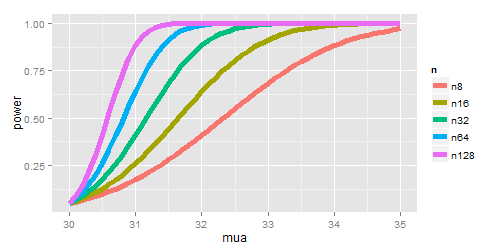
\includegraphics{LeanPub/images/powerCurve-1.png}
\caption{Plot of power as $\mu_a$ varies.}
\end{figure}

The code below shows how to use manipulate to investigate power as the
various inputs change.

\vspace{1pc}

\verb;Code for investigating power.:;

\begin{Shaded}
\begin{Highlighting}[]
\KeywordTok{library}\NormalTok{(manipulate)}
\NormalTok{mu0 =}\StringTok{ }\DecValTok{30}
\NormalTok{myplot <-}\StringTok{ }\NormalTok{function(sigma, mua, n, alpha) \{}
    \NormalTok{g =}\StringTok{ }\KeywordTok{ggplot}\NormalTok{(}\KeywordTok{data.frame}\NormalTok{(}\DataTypeTok{mu =} \KeywordTok{c}\NormalTok{(}\DecValTok{27}\NormalTok{, }\DecValTok{36}\NormalTok{)), }\KeywordTok{aes}\NormalTok{(}\DataTypeTok{x =} \NormalTok{mu))}
    \NormalTok{g =}\StringTok{ }\NormalTok{g +}\StringTok{ }\KeywordTok{stat_function}\NormalTok{(}\DataTypeTok{fun =} \NormalTok{dnorm, }\DataTypeTok{geom =} \StringTok{"line"}\NormalTok{,}
                          \DataTypeTok{args =} \KeywordTok{list}\NormalTok{(}\DataTypeTok{mean =} \NormalTok{mu0,}
        \DataTypeTok{sd =} \NormalTok{sigma/}\KeywordTok{sqrt}\NormalTok{(n)), }\DataTypeTok{size =} \DecValTok{2}\NormalTok{, }\DataTypeTok{col =} \StringTok{"red"}\NormalTok{)}
    \NormalTok{g =}\StringTok{ }\NormalTok{g +}\StringTok{ }\KeywordTok{stat_function}\NormalTok{(}\DataTypeTok{fun =} \NormalTok{dnorm, }\DataTypeTok{geom =} \StringTok{"line"}\NormalTok{,}
                          \DataTypeTok{args =} \KeywordTok{list}\NormalTok{(}\DataTypeTok{mean =} \NormalTok{mua,}
        \DataTypeTok{sd =} \NormalTok{sigma/}\KeywordTok{sqrt}\NormalTok{(n)), }\DataTypeTok{size =} \DecValTok{2}\NormalTok{, }\DataTypeTok{col =} \StringTok{"blue"}\NormalTok{)}
    \NormalTok{xitc =}\StringTok{ }\NormalTok{mu0 +}\StringTok{ }\KeywordTok{qnorm}\NormalTok{(}\DecValTok{1} \NormalTok{-}\StringTok{ }\NormalTok{alpha) *}\StringTok{ }\NormalTok{sigma/}\KeywordTok{sqrt}\NormalTok{(n)}
    \NormalTok{g =}\StringTok{ }\NormalTok{g +}\StringTok{ }\KeywordTok{geom_vline}\NormalTok{(}\DataTypeTok{xintercept =} \NormalTok{xitc, }\DataTypeTok{size =} \DecValTok{3}\NormalTok{)}
    \NormalTok{g}
\NormalTok{\}}
\KeywordTok{manipulate}\NormalTok{(}\KeywordTok{myplot}\NormalTok{(sigma, mua, n, alpha),}
           \DataTypeTok{sigma =} \KeywordTok{slider}\NormalTok{(}\DecValTok{1}\NormalTok{, }\DecValTok{10}\NormalTok{, }\DataTypeTok{step =} \DecValTok{1}\NormalTok{, }\DataTypeTok{initial =} \DecValTok{4}\NormalTok{),}
    \DataTypeTok{mua =} \KeywordTok{slider}\NormalTok{(}\DecValTok{30}\NormalTok{, }\DecValTok{35}\NormalTok{, }\DataTypeTok{step =} \DecValTok{1}\NormalTok{, }\DataTypeTok{initial =} \DecValTok{32}\NormalTok{),}
    \DataTypeTok{n =} \KeywordTok{slider}\NormalTok{(}\DecValTok{1}\NormalTok{, }\DecValTok{50}\NormalTok{, }\DataTypeTok{step =} \DecValTok{1}\NormalTok{, }\DataTypeTok{initial =} \DecValTok{16}\NormalTok{),}
    \DataTypeTok{alpha =} \KeywordTok{slider}\NormalTok{(}\FloatTok{0.01}\NormalTok{, }\FloatTok{0.1}\NormalTok{, }\DataTypeTok{step =} \FloatTok{0.01}\NormalTok{, }\DataTypeTok{initial =} \FloatTok{0.05}\NormalTok{))}
\end{Highlighting}
\end{Shaded}

\subsection{Question}\label{question}

\href{http://youtu.be/3bWhP5MyuqI?list=PLpl-gQkQivXiBmGyzLrUjzsblmQsLtkzJ}{Watch
this video before beginning.}

When testing $H_a : \mu > \mu_0$, notice if power is $1 - \beta$, then

\[1 - \beta = P\left(\bar X > \mu_0 + z_{1-\alpha} \frac{\sigma}{\sqrt{n}} ; \mu = \mu_a \right)\]

where $\bar X \sim N(\mu_a, \sigma^2 / n)$. The unknowns in the equation
are: $\mu_a$, $\sigma$, $n$, $\beta$ and the knowns are: $\mu_0$,
$\alpha$. Specify any 3 of the unknowns and you can solve for the
remainder.

\subsection{Notes}\label{notes}

\begin{itemize}
\itemsep1pt\parskip0pt\parsep0pt
\item
  The calculation for $H_a:\mu < \mu_0$ is similar
\item
  For $H_a: \mu \neq \mu_0$ calculate the one sided power using
  $\alpha / 2$ (this is only approximately right, it excludes the
  probability of getting a large TS in the opposite direction of the
  truth)
\item
  Power goes up as $\alpha$ gets larger
\item
  Power of a one sided test is greater than the power of the associated
  two sided test
\item
  Power goes up as $\mu_1$ gets further away from $\mu_0$
\item
  Power goes up as $n$ goes up
\item
  Power doesn't need $\mu_a$, $\sigma$ and $n$, instead only
  $\frac{\sqrt{n}(\mu_a - \mu_0)}{\sigma}$
\item
  The quantity $\frac{\mu_a - \mu_0}{\sigma}$ is called the \emph{effect
  size}, the difference in the means in standard deviation units.
\item
  Being unit free, it has some hope of interpretability across settings.
\end{itemize}

\subsection{T-test power}\label{t-test-power}

\href{http://youtu.be/1DiwutNpt5Y?list=PLpl-gQkQivXiBmGyzLrUjzsblmQsLtkzJ}{Watch
this before beginning.}

Consider calculating power for a Gosset's \emph{t} test for our example
where we now assume that $n=16$. The power is

\[
P\left(\frac{\bar X - \mu_0}{S /\sqrt{n}} > t_{1-\alpha, n-1} ~;~ \mu = \mu_a \right).
\]

Calculating this requires the so-called non-central t distribution.
However, fortunately for us, the R function \texttt{power.t.test} does
this very well. Omit (exactly) any one of the arguments and it solves
for it. Our t-test power again only relies on the effect size.

Let's do our example trying different options.

\vspace{1pc}

\verb;Example of using 'power.t.test' in R.:;

\begin{Shaded}
\begin{Highlighting}[]
\CommentTok{# omitting the power and getting a power estimate}
\KeywordTok{power.t.test}\NormalTok{(}\DataTypeTok{n =} \DecValTok{16}\NormalTok{, }\DataTypeTok{delta =} \DecValTok{2}\NormalTok{/}\DecValTok{4}\NormalTok{, }\DataTypeTok{sd =} \DecValTok{1}\NormalTok{,}
             \DataTypeTok{type =} \StringTok{"one.sample"}\NormalTok{, }\DataTypeTok{alt =} \StringTok{"one.sided"}\NormalTok{)$power}
\end{Highlighting}
\end{Shaded}

\begin{verbatim}
## [1] 0.6040329
\end{verbatim}

\begin{Shaded}
\begin{Highlighting}[]
\CommentTok{# illustrating that it depends only on the effect size, delta/sd}
\KeywordTok{power.t.test}\NormalTok{(}\DataTypeTok{n =} \DecValTok{16}\NormalTok{, }\DataTypeTok{delta =} \DecValTok{2}\NormalTok{, }\DataTypeTok{sd =} \DecValTok{4}\NormalTok{,}
             \DataTypeTok{type =} \StringTok{"one.sample"}\NormalTok{, }\DataTypeTok{alt =} \StringTok{"one.sided"}\NormalTok{)$power}
\end{Highlighting}
\end{Shaded}

\begin{verbatim}
## [1] 0.6040329
\end{verbatim}

\begin{Shaded}
\begin{Highlighting}[]
\CommentTok{# same thing again}
\KeywordTok{power.t.test}\NormalTok{(}\DataTypeTok{n =} \DecValTok{16}\NormalTok{, }\DataTypeTok{delta =} \DecValTok{100}\NormalTok{, }\DataTypeTok{sd =} \DecValTok{200}\NormalTok{,}
             \DataTypeTok{type =} \StringTok{"one.sample"}\NormalTok{, }\DataTypeTok{alt =} \StringTok{"one.sided"}\NormalTok{)$power}
\end{Highlighting}
\end{Shaded}

\begin{verbatim}
## [1] 0.6040329
\end{verbatim}

\begin{Shaded}
\begin{Highlighting}[]
\CommentTok{# specifying the power and getting n}
\KeywordTok{power.t.test}\NormalTok{(}\DataTypeTok{power =} \FloatTok{0.8}\NormalTok{, }\DataTypeTok{delta =} \DecValTok{2}\NormalTok{/}\DecValTok{4}\NormalTok{, }\DataTypeTok{sd =} \DecValTok{1}\NormalTok{,}
             \DataTypeTok{type =} \StringTok{"one.sample"}\NormalTok{, }\DataTypeTok{alt =} \StringTok{"one.sided"}\NormalTok{)$n}
\end{Highlighting}
\end{Shaded}

\begin{verbatim}
## [1] 26.13751
\end{verbatim}

\begin{Shaded}
\begin{Highlighting}[]
\CommentTok{# again illustrating that the effect size is all that matters}
\KeywordTok{power.t.test}\NormalTok{(}\DataTypeTok{power =} \FloatTok{0.8}\NormalTok{, }\DataTypeTok{delta =} \DecValTok{2}\NormalTok{, }\DataTypeTok{sd =} \DecValTok{4}\NormalTok{,}
             \DataTypeTok{type =} \StringTok{"one.sample"}\NormalTok{, }\DataTypeTok{alt =} \StringTok{"one.sided"}\NormalTok{)$n}
\end{Highlighting}
\end{Shaded}

\begin{verbatim}
## [1] 26.13751
\end{verbatim}

\begin{Shaded}
\begin{Highlighting}[]
\CommentTok{# again illustrating that the effect size is all that matters}
\KeywordTok{power.t.test}\NormalTok{(}\DataTypeTok{power =} \FloatTok{0.8}\NormalTok{, }\DataTypeTok{delta =} \DecValTok{100}\NormalTok{, }\DataTypeTok{sd =} \DecValTok{200}\NormalTok{,}
             \DataTypeTok{type =} \StringTok{"one.sample"}\NormalTok{, }\DataTypeTok{alt =} \StringTok{"one.sided"}\NormalTok{)$n}
\end{Highlighting}
\end{Shaded}

\begin{verbatim}
## [1] 26.13751
\end{verbatim}

\subsection{Exercises}\label{exercises-10}

\begin{enumerate}
\def\labelenumi{\arabic{enumi}.}
\itemsep1pt\parskip0pt\parsep0pt
\item
  Power is a probability calculation assuming which is true:
\end{enumerate}

\begin{itemize}
\itemsep1pt\parskip0pt\parsep0pt
\item
  The null hypothesis
\item
  The alternative hypothesis
\item
  Both the null and alternative
\end{itemize}

\begin{enumerate}
\def\labelenumi{\arabic{enumi}.}
\setcounter{enumi}{1}
\itemsep1pt\parskip0pt\parsep0pt
\item
  As your sample size gets bigger, all else equal, what do you think
  would happen to power?
\end{enumerate}

\begin{itemize}
\itemsep1pt\parskip0pt\parsep0pt
\item
  It would get larger
\item
  It would get smaller
\item
  It would stay the same
\item
  It cannot be determined from the information given
\end{itemize}

\begin{enumerate}
\def\labelenumi{\arabic{enumi}.}
\setcounter{enumi}{2}
\itemsep1pt\parskip0pt\parsep0pt
\item
  What happens to power as $\mu_a$ gets further from $\mu_0$?
\end{enumerate}

\begin{itemize}
\itemsep1pt\parskip0pt\parsep0pt
\item
  Power decreases
\item
  Power increases
\item
  Power stays the same
\item
  Power oscillates
\end{itemize}

\begin{enumerate}
\def\labelenumi{\arabic{enumi}.}
\setcounter{enumi}{3}
\itemsep1pt\parskip0pt\parsep0pt
\item
  In the context of calculating power, the effect size is?
\end{enumerate}

\begin{itemize}
\itemsep1pt\parskip0pt\parsep0pt
\item
  The null mean divided by the standard deviation
\item
  The alternative mean divided by the standard error
\item
  The difference between the null and alternative means divided by the
  standard deviation
\item
  The standard error divided by the null mean
\end{itemize}

\begin{enumerate}
\def\labelenumi{\arabic{enumi}.}
\setcounter{enumi}{4}
\itemsep1pt\parskip0pt\parsep0pt
\item
  Recall this problem ``Suppose that in an AB test, one advertising
  scheme led to an average of 10 purchases per day for a sample of 100
  days, while the other led to 11 purchases per day, also for a sample
  of 100 days. Assuming a common standard deviation of 4 purchases per
  day.'' Assuming that 10 purchases per day is a benchmark null value,
  that days are iid and that the standard deviation is 4 purchases for
  day. Suppose that you plan on sampling 100 days. What would be the
  power for a one sided 5\% Z mean test that purchases per day have
  increased under the alternative of $\mu = 11$ purchase per day?
  \href{https://www.youtube.com/watch?v=RiS6EFnPYY8\&index=34\&list=PLpl-gQkQivXhHOcVeU3bSJg78zaDYbP9L}{Watch
  a video solution} and
  \href{http://bcaffo.github.io/courses/06_StatisticalInference/homework/hw4.html\#10}{see
  the text}.
\item
  Researchers would like to conduct a study of healthy adults to detect
  a four year mean brain volume loss of .01 mm3. Assume that the
  standard deviation of four year volume loss in this population is .04
  mm3. What is necessary sample size for the study for a 5\% one sided
  test versus a null hypothesis of no volume loss to achieve 80\% power?
  \href{https://www.youtube.com/watch?v=lrXyJrtatzk\&index=35\&list=PLpl-gQkQivXhHOcVeU3bSJg78zaDYbP9L}{Watch
  the video solution} and
  \href{http://bcaffo.github.io/courses/06_StatisticalInference/homework/hw4.html\#11}{see
  the text}.
\end{enumerate}

\newpage

\section{The bootstrap and
resampling}\label{the-bootstrap-and-resampling}

\subsection{The bootstrap}\label{the-bootstrap}

\href{http://youtu.be/0hNQx9nagq4?list=PLpl-gQkQivXiBmGyzLrUjzsblmQsLtkzJ}{Watch
this video before beginning.}

The bootstrap is a tremendously useful tool for constructing confidence
intervals and calculating standard errors for difficult statistics. For
a classic example, how would one derive a confidence interval for the
median? The bootstrap procedure follows from the so called bootstrap
principle

To illustrate the bootstrap principle, imagine a die roll. The image
below shows the mass function of a die roll on the left. On the right we
show the empirical distribution obtained by repeatedly averaging 50
independent die rolls. By this simulation, without any mathematics, we
have a good idea of what the distribution of averages of 50 die rolls
looks like.

\begin{figure}[htbp]
\centering
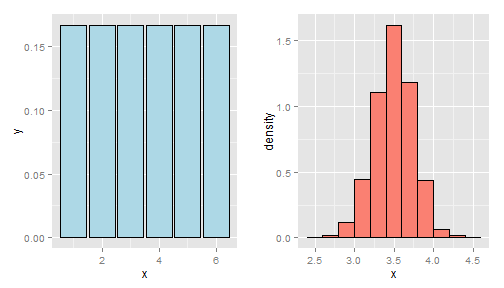
\includegraphics{LeanPub/images/bootstrapping1-1.png}
\caption{Image of true die roll distribution (left) and simulation of
averages of 50 die rolls}
\end{figure}

Now imagine a case where we didn't know whether or not the die was fair.
We have a sample of size 50 and we'd like to investigate the
distribution of the average of 50 die rolls \emph{where we're not
allowed to roll the die anymore}. This is more like a real data
analysis, we only get one sample from the population.

\begin{figure}[htbp]
\centering
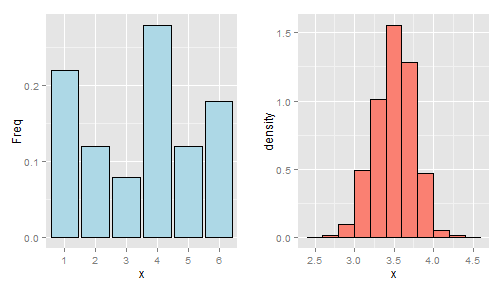
\includegraphics{LeanPub/images/bootstrapping2-1.png}
\caption{Image of empirical die roll distribution (left) and simulates
of averages of 50 die rolls from this distribution}
\end{figure}

The bootstrap principle is to use the empirical mass function of the
data to perform the simulation, rather than the true distribution. That
is, we simulate averages of 50 samples from the histogram that we
observe. With enough data, the empirical distribution should be a good
estimate of the true distribution and this should result in a good
approximation of the sampling distribution.

That's the bootstrap principle: investigate the sampling distribution of
a statistic by simulating repeated realizations from the observed
distribution.

If we could simulate from the true distribution, then we would know the
exact sampling distribution of our statistic (if we ran our computer
long enough.) However, since we only get to sample from that
distribution once, we have to be content with using the empirical
distribution. This is the clever idea of the bootstrap.

\subsubsection{Example Galton's fathers and sons
dataset}\label{example-galtons-fathers-and-sons-dataset}

\href{http://youtu.be/yNTWcmbWvWg?list=PLpl-gQkQivXiBmGyzLrUjzsblmQsLtkzJ}{Watch
this video before beginning.}

The code below creates resamples via draws of size n with replacement
with the original data of the son's heights from Galton's data and plots
a histogram of the median of each resampled dataset.

\vspace{1pc}

\verb;Bootstrapping example:;

\begin{Shaded}
\begin{Highlighting}[]
\KeywordTok{library}\NormalTok{(UsingR)}
\KeywordTok{data}\NormalTok{(father.son)}
\NormalTok{x <-}\StringTok{ }\NormalTok{father.son$sheight}
\NormalTok{n <-}\StringTok{ }\KeywordTok{length}\NormalTok{(x)}
\NormalTok{B <-}\StringTok{ }\DecValTok{10000}
\NormalTok{resamples <-}\StringTok{ }\KeywordTok{matrix}\NormalTok{(}\KeywordTok{sample}\NormalTok{(x, n *}\StringTok{ }\NormalTok{B, }\DataTypeTok{replace =} \OtherTok{TRUE}\NormalTok{), B, n)}
\NormalTok{resampledMedians <-}\StringTok{ }\KeywordTok{apply}\NormalTok{(resamples, }\DecValTok{1}\NormalTok{, median)}
\end{Highlighting}
\end{Shaded}

\begin{figure}[htbp]
\centering
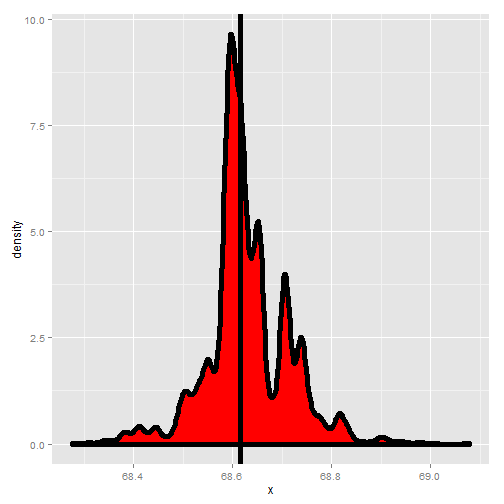
\includegraphics{LeanPub/images/bootstrapping3-1.png}
\caption{Bootstrapping example for the median of sons' heights from
Galton's}
\end{figure}

\subsection{The bootstrap principle}\label{the-bootstrap-principle}

\href{http://youtu.be/BKrMjX7FBno?list=PLpl-gQkQivXiBmGyzLrUjzsblmQsLtkzJ}{Watch
this video before beginning.}

Suppose that I have a statistic that estimates some population
parameter, but I don't know its sampling distribution. The bootstrap
principle suggests using the distribution defined by the data to
approximate its sampling distribution

\subsubsection{The bootstrap in
practice}\label{the-bootstrap-in-practice}

In practice, the bootstrap principle is always carried out using
simulation. We will cover only a few aspects of bootstrap resampling.
The general procedure follows by first simulating complete data sets
from the observed data with replacement. This is approximately drawing
from the sampling distribution of that statistic, at least as far as the
data is able to approximate the true population distribution. Calculate
the statistic for each simulated data set Use the simulated statistics
to either define a confidence interval or take the standard deviation to
calculate a standard error.

\subsubsection{Nonparametric bootstrap algorithm
example}\label{nonparametric-bootstrap-algorithm-example}

Bootstrap procedure for calculating confidence interval for the median
from a data set of $n$ observations:

\begin{enumerate}
\def\labelenumi{\arabic{enumi}.}
\item
  Sample $n$ observations \textbf{with replacement} from the observed
  data resulting in one simulated complete data set.
\item
  Take the median of the simulated data set
\item
  Repeat these two steps $B$ times, resulting in $B$ simulated medians
\item
  These medians are approximately drawn from the sampling distribution
  of the median of $n$ observations; therefore we can:

  \begin{itemize}
  \itemsep1pt\parskip0pt\parsep0pt
  \item
    Draw a histogram of them
  \item
    Calculate their standard deviation to estimate the standard error of
    the median
  \item
    Take the $2.5^{th}$ and $97.5^{th}$ percentiles as a confidence
    interval for the median
  \end{itemize}
\end{enumerate}

For the general bootstrap, just replace the median with whatever
statistic that you're investigating.

\subsubsection{Example code}\label{example-code}

Consider our father/son data from before. Here is the relevant code for
doing the resampling.

\begin{Shaded}
\begin{Highlighting}[]
\NormalTok{B <-}\StringTok{ }\DecValTok{10000}
\NormalTok{resamples <-}\StringTok{ }\KeywordTok{matrix}\NormalTok{(}\KeywordTok{sample}\NormalTok{(x,}
                           \NormalTok{n *}\StringTok{ }\NormalTok{B,}
                           \DataTypeTok{replace =} \OtherTok{TRUE}\NormalTok{),}
                    \NormalTok{B, n)}
\NormalTok{medians <-}\StringTok{ }\KeywordTok{apply}\NormalTok{(resamples, }\DecValTok{1}\NormalTok{, median)}
\end{Highlighting}
\end{Shaded}

And here is some results.

\begin{Shaded}
\begin{Highlighting}[]
\KeywordTok{sd}\NormalTok{(medians)}
\end{Highlighting}
\end{Shaded}

\begin{verbatim}
## [1] 0.0847079
\end{verbatim}

Thus, 0.084 estimates the standard error of the median for this data
set. It did this by repeatedly sampling medians from the observed
distribution and taking the standard deviation of the resulting
collection of medians. Taking the 2.5 and 97.5 percentiles gives us a
bootstrap 95\% confidence interval for the median.

\begin{Shaded}
\begin{Highlighting}[]
\KeywordTok{quantile}\NormalTok{(medians, }\KeywordTok{c}\NormalTok{(.}\DecValTok{025}\NormalTok{, .}\DecValTok{975}\NormalTok{))}
\end{Highlighting}
\end{Shaded}

\begin{verbatim}
##     2.5%    97.5% 
## 68.42972 68.81509
\end{verbatim}

We also always want to plot a histogram or density estimate of our
simulated statistic.

\begin{Shaded}
\begin{Highlighting}[]
\NormalTok{g =}\StringTok{ }\KeywordTok{ggplot}\NormalTok{(}\KeywordTok{data.frame}\NormalTok{(}\DataTypeTok{medians =} \NormalTok{medians), }\KeywordTok{aes}\NormalTok{(}\DataTypeTok{x =} \NormalTok{medians))}
\NormalTok{g =}\StringTok{ }\NormalTok{g +}\StringTok{ }\KeywordTok{geom_histogram}\NormalTok{(}\DataTypeTok{color =} \StringTok{"black"}\NormalTok{, }\DataTypeTok{fill =} \StringTok{"lightblue"}\NormalTok{,}
                       \DataTypeTok{binwidth =} \FloatTok{0.05}\NormalTok{)}
\NormalTok{g}
\end{Highlighting}
\end{Shaded}

\begin{figure}[htbp]
\centering
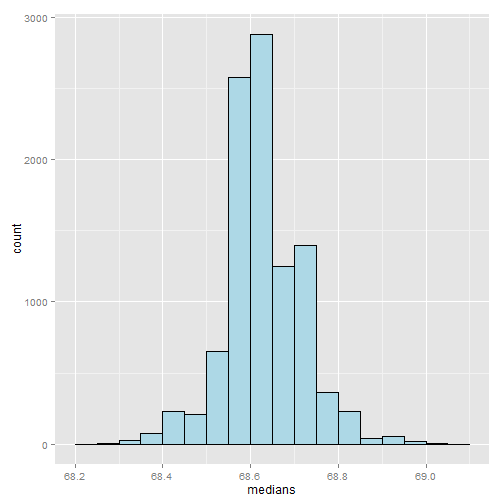
\includegraphics{LeanPub/images/bootstrapping4-1.png}
\caption{A plot of the histrogram of the resamples}
\end{figure}

\subsubsection{Summary notes on the
bootstrap}\label{summary-notes-on-the-bootstrap}

\begin{itemize}
\itemsep1pt\parskip0pt\parsep0pt
\item
  The bootstrap is non-parametric.
\item
  Better percentile bootstrap confidence intervals correct for bias.
\item
  There are lots of variations on bootstrap procedures; the book
  \href{http://www.crcpress.com/product/isbn/9780412042317}{An
  Introduction to the Bootstrap} by Efron and Tibshirani is a great
  place to start for both bootstrap and jackknife information.
\end{itemize}

\subsection{Group comparisons via permutation
tests}\label{group-comparisons-via-permutation-tests}

\href{http://youtu.be/nn1t9Kk7nn8?list=PLpl-gQkQivXiBmGyzLrUjzsblmQsLtkzJ}{Watch
this video before beginning.}

Consider comparing two independent groups. Example, comparing sprays B
and C.

\begin{Shaded}
\begin{Highlighting}[]
\KeywordTok{data}\NormalTok{(InsectSprays)}
\NormalTok{g =}\StringTok{ }\KeywordTok{ggplot}\NormalTok{(InsectSprays, }\KeywordTok{aes}\NormalTok{(spray, count, }\DataTypeTok{fill =} \NormalTok{spray))}
\NormalTok{g =}\StringTok{ }\NormalTok{g +}\StringTok{ }\KeywordTok{geom_boxplot}\NormalTok{()}
\NormalTok{g}
\end{Highlighting}
\end{Shaded}

\begin{figure}[htbp]
\centering
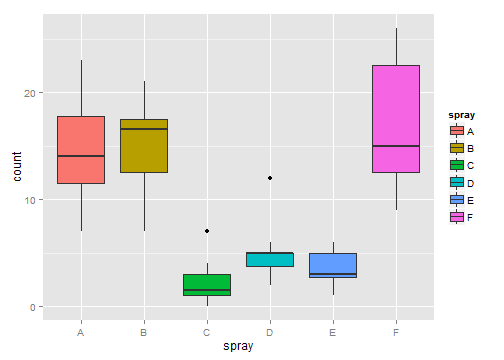
\includegraphics{LeanPub/images/bootstrapping5-1.png}
\caption{Comparison of insect spray.}
\end{figure}

\subsection{Permutation tests}\label{permutation-tests}

Consider comparing means between the group. However, let's use the
calculate the distribution of our statistic under a null hypothesis that
the labels are irrelevant (exchangeable). This is a handy way to create
a null distribution for our test statistic by simply permuting the
labels over and over and seeing how extreme our data are with respect to
this permuted distribution.

The procedure would be as follows:

\begin{enumerate}
\def\labelenumi{\arabic{enumi}.}
\itemsep1pt\parskip0pt\parsep0pt
\item
  consider a data from with count and spray,
\item
  permute the spray (group) labels,
\item
  recalculate the statistic (such as the difference in means),
\item
  calculate the percentage of simulations where the simulated statistic
  was more extreme (toward the alternative) than the observed.
\end{enumerate}

\subsection{Variations on permutation
testing}\label{variations-on-permutation-testing}

This idea of exchangeability of the group labels is so powerful, that
it's been reinvented several times in statistic. The table below gives
three famous tests that are obtained by permuting group labels.

\begin{longtable}[c]{@{}lll@{}}
\toprule\addlinespace
Data type & Statistic & Test name
\\\addlinespace
\midrule\endhead
Ranks & rank sum & rank sum test
\\\addlinespace
Binary & hypergeometric prob & Fisher's exact test
\\\addlinespace
Raw data & & permutation test
\\\addlinespace
\bottomrule
\end{longtable}

Also, so-called \emph{randomization tests} are exactly permutation
tests, with a different motivation. In that case, think of the
permutation test as replicating the random assignment over and over.

For matched or paired data, it wouldn't make sense to randomize the
group labels, since that would break the association between the pairs.
Instead, one can randomize the signs of the pairs. For data that has
been replaced by ranks, you might of heard of this test before as the
the signed rank test.

Again we won't cover more complex examples, but it should be said that
permutation strategies work for regression as well by permuting a
regressor of interest (though this needs to be done with care). These
tests work very well in massively multivariate settings.

\subsection{Permutation test B v C}\label{permutation-test-b-v-c}

Let's create some code for our example. Our statistic will be the
difference in the means in each group.

\vspace{1pc}

\verb;Permutation distribution for the insect sprays dataset.:;

\begin{Shaded}
\begin{Highlighting}[]
\NormalTok{subdata <-}\StringTok{ }\NormalTok{InsectSprays[InsectSprays$spray %in%}\StringTok{ }\KeywordTok{c}\NormalTok{(}\StringTok{"B"}\NormalTok{, }\StringTok{"C"}\NormalTok{),]}
\NormalTok{y <-}\StringTok{ }\NormalTok{subdata$count}
\NormalTok{group <-}\StringTok{ }\KeywordTok{as.character}\NormalTok{(subdata$spray)}
\NormalTok{testStat <-}\StringTok{ }\NormalTok{function(w, g) }\KeywordTok{mean}\NormalTok{(w[g ==}\StringTok{ "B"}\NormalTok{]) -}\StringTok{ }\KeywordTok{mean}\NormalTok{(w[g ==}\StringTok{ "C"}\NormalTok{])}
\NormalTok{observedStat <-}\StringTok{ }\KeywordTok{testStat}\NormalTok{(y, group)}
\NormalTok{permutations <-}\StringTok{ }\KeywordTok{sapply}\NormalTok{(}\DecValTok{1} \NormalTok{:}\StringTok{ }\DecValTok{10000}\NormalTok{,}
                       \NormalTok{function(i) }\KeywordTok{testStat}\NormalTok{(y, }\KeywordTok{sample}\NormalTok{(group)))}
\end{Highlighting}
\end{Shaded}

Let's look at some of the results. First let's look at the observed
statistic.

\begin{Shaded}
\begin{Highlighting}[]
\NormalTok{observedStat}
\end{Highlighting}
\end{Shaded}

\begin{verbatim}
## [1] 13.25
\end{verbatim}

Now let's see what proportion of times we got a simulated statistic
larger than our observed statistic.

\begin{Shaded}
\begin{Highlighting}[]
\KeywordTok{mean}\NormalTok{(permutations >}\StringTok{ }\NormalTok{observedStat)}
\end{Highlighting}
\end{Shaded}

\begin{verbatim}
## [1] 0
\end{verbatim}

Since this is 0, our estimate of the P-value is 0 (i.e.~we strongly
reject the NULL). It's useful to look at a histogram of permuted
statistics with a vertical line drawn at the observed test statistic for
reference.

\begin{figure}[htbp]
\centering
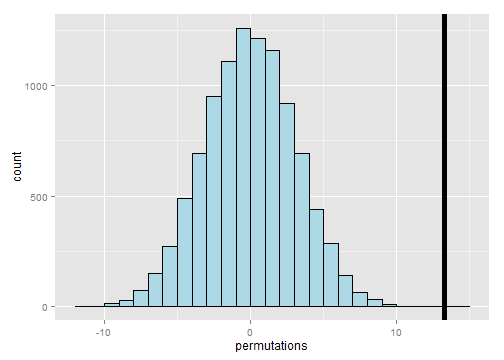
\includegraphics{LeanPub/images/bootstrapping6-1.png}
\caption{Permutation distribution from the insectsprays dataset}
\end{figure}

\subsection{Exercises}\label{exercises-11}

\begin{enumerate}
\def\labelenumi{\arabic{enumi}.}
\itemsep1pt\parskip0pt\parsep0pt
\item
  The bootstrap uses what to estimate the sampling distribution of a
  statistic?
\end{enumerate}

\begin{itemize}
\itemsep1pt\parskip0pt\parsep0pt
\item
  The true population distribution
\item
  The empirical distribution that puts probability 1/n for each observed
  data point
\end{itemize}

\begin{enumerate}
\def\labelenumi{\arabic{enumi}.}
\setcounter{enumi}{1}
\itemsep1pt\parskip0pt\parsep0pt
\item
  When performing the bootstrap via Monte Carlo resampling for a data
  set of size n which is true? Assume that you're going to do 10,000
  bootstrap resamples?
\end{enumerate}

\begin{itemize}
\itemsep1pt\parskip0pt\parsep0pt
\item
  You sample n complete data sets of size 10,000 with replacement
\item
  You sample 10,000 complete data sets of size n without replacement
\item
  You sample 10,000 complete data sets of size n with replacement
\item
  You sample n complete data sets of size 10,000 without replacement
\end{itemize}

\begin{enumerate}
\def\labelenumi{\arabic{enumi}.}
\setcounter{enumi}{2}
\itemsep1pt\parskip0pt\parsep0pt
\item
  Permutation tests do what?
\end{enumerate}

\begin{itemize}
\itemsep1pt\parskip0pt\parsep0pt
\item
  Creates a null distribution for a hypothesis test by permuting a
  predictor variable.
\item
  Creates a null distribution by resampling from the response with
  replacement.
\item
  Creates an alternative distribution by permuting group labels.
\item
  Creates confidence intervals by resampling with replacement.
\end{itemize}

\end{document}
